% Paper 1: Gradient-Free Retrieval Weight Learning via Thompson Sampling
% Target: arXiv preprint (cs.IR), ICML 2026 workshops
% Format: No page limit

\documentclass[10pt]{article}
\usepackage[preprint]{tmlr}
\usepackage{url}
\usepackage{amsmath}
\usepackage{amssymb}
\usepackage{graphicx}
\usepackage{booktabs}
\usepackage{multirow}
\usepackage{xcolor}
\usepackage{algorithm}
\usepackage{algpseudocode}
\usepackage{hyperref}

% Metadata (unused in preprint mode, required by tmlr.sty)
\def\month{03}
\def\year{2026}
\def\openreview{}

% Custom commands
\newcommand{\tsscore}{\text{score}}
\newcommand{\wpreset}{\mathbf{w}}
\newcommand{\dimR}{\text{R}}  % recency
\newcommand{\dimI}{\text{I}}  % importance
\newcommand{\dimV}{\text{V}}  % relevance

\title{Gradient-Free Retrieval Weight Learning via Thompson Sampling with LLM Self-Assessment}

\author{\name Alfonso A.~V.~DiRocco \email alfonso@kusp.dev \\
  \addr Kusp}

\begin{document}
\maketitle

\begin{abstract}
% Abstract — ~250 words
% NOTE: Updated with v3 re-run results (2026-03-11)

Retrieval-augmented agent systems typically combine retrieval dimensions (recency, importance, and relevance) using fixed, hand-tuned weights.
Park et al.\ (2023) hardcoded equal weights ($w^R = w^I = w^V = 1/3$), an assumption that has gone unchallenged.
We present a gradient-free method for learning these weights online via Thompson Sampling over discrete weight presets, where reward comes from LLM self-assessment of \emph{retrieval input quality}, not task output quality.
This metalevel input assessment---evaluating the system's retrieval choices rather than its generation quality---is designed to avoid the reward hacking identified by Pan et al.\ (2024), where output-level self-assessment inflates scores while quality stagnates.
While recent work on agentic search, long-context models, and retrieval internalization via fine-tuning suggests that vector-based retrieval may not remain the dominant paradigm for small corpora, the mechanisms we study---gradient-free parameter learning and non-hackable self-assessment---are in principle architecture-agnostic and may apply wherever systems must learn configuration parameters online without labeled data.
Across 1{,}200 episodes (300 tasks $\times$ 4 conditions, 205 domain-specific skills), feedback-guided retrieval reduces token consumption by 12--20\% versus the no-feedback control (Kruskal--Wallis $H(3){=}33.87$, $p{<}0.001$; all treatment-vs-control comparisons significant after Holm--Bonferroni correction).
The mechanism is output-driven: feedback conditions produce shorter, more targeted LLM responses (control mean output 3{,}813 tokens vs.\ 2{,}537 for the best treatment, a 33\% reduction), consistent with more focused prompts from better-weighted retrieval.
The full system with explanation embeddings achieves the strongest retrieval quality (NDCG@5 $= 0.469$, +26.3\% vs.\ control; MRR $= 0.411$, +35.9\% vs.\ control), while the qualitative anchor condition yields the largest token savings ($-19.7\%$).
Convergence analysis reveals interpretable specialization: the full system converges to a pure-relevance preset (posterior mean 0.749), while qualitative anchors converge toward pure-importance (0.472).
Skill-set overlap across conditions (Jaccard ${\sim}$0.52--0.59) confirms that learned weight configurations produce meaningfully differentiated retrieval.

Our contributions are: (1)~a gradient-free method for online retrieval weight learning in agent memory systems; (2)~empirical evidence of an output-driven efficiency effect associated with improved retrieval quality; (3)~a diagnostic framework revealing when weight learning fails and how to fix it; and (4)~evidence that metalevel input assessment avoids output-level reward hacking.

\end{abstract}

\section{Introduction}
\label{sec:introduction}
% Section 1: Introduction (~1.25 pages)

Agentic LLM systems increasingly rely on retrieval to inject relevant context (skills, memories, tools) at inference time.
The dominant architecture for memory retrieval in generative agents, introduced by~\citet{park2023generative}, combines three scoring dimensions with fixed equal weights:
\begin{equation}
\tsscore(s) = \frac{1}{3}\dimR(s) + \frac{1}{3}\dimI(s) + \frac{1}{3}\dimV(s)
\label{eq:park_baseline}
\end{equation}
where $\dimR$ captures recency (linear decay over iterations since last use, clamped at zero), $\dimI$ captures importance (historical success rate), and $\dimV$ captures relevance (embedding similarity to the current task).
This equal-weight assumption has been adopted without question in subsequent work, despite the intuition that different tasks demand different retrieval priorities: a debugging task benefits from proven solutions ($\dimI$-heavy), while a trend analysis task benefits from recent information ($\dimR$-heavy).

These weights represent an unexplored optimization target.
Unlike retrieval strategy selection~\citep{tang2025mbarag,jeong2024adaptiverag} or retriever model training~\citep{asai2024selfrag}, no prior work learns the \emph{weighting parameters within a single retrieval scoring function} online during deployment.

The central challenge is obtaining a reward signal without task-level ground truth.
One natural approach, having the LLM rate its own output quality, leads to reward hacking:~\citet{pan2024feedback} showed that when LLM-generated scores feed back into the system that produced them, scores inflate while actual quality stagnates or degrades.
Our key insight is to assess \emph{input quality} rather than \emph{output quality}: the rubric asks ``how useful was the retrieved context for this task?'' rather than ``how good was my response?''
This metalevel judgment---assessing the system's inputs rather than its outputs---does not directly optimize the evaluated signal, avoiding the self-referential feedback loop that enables reward hacking.

We operationalize this insight through Thompson Sampling~\citep{thompson1933likelihood,chapelle2011empirical} over a discrete set of weight presets.
Each preset $\wpreset_k = (w_k^R, w_k^I, w_k^V)$ defines a configuration on the weight simplex.
After each task, the LLM provides dimension-specific Likert ratings of retrieval quality, which are aggregated into a composite reward for Bayesian posterior updating.
Over episodes, presets that produce context rated as more useful accumulate evidence and are selected more frequently.

We present two experiments with contrasting findings:

\paragraph{Experiment 1 (v2)} reveals a confounded design.
Across 250 tasks with 50 generic skills, feedback-guided retrieval reduces mean token consumption by 40--50\% (bootstrap $p \leq 0.012$), but skill overlap between conditions remains 85--91\%, indicating that learned weights do not change what gets retrieved.
We diagnose the root cause: with only 50 generic skills, the recency and importance dimensions are near-saturated (${\sim}$0.95), leaving insufficient variance for weight differences to affect rankings.
The token savings appear driven by the feedback rubric itself rather than by weight adaptation, motivating the redesigned v3 experiment.

\paragraph{Experiment 2 (v3)} corrects the design flaws identified in v2 and provides evidence that weight learning genuinely improves retrieval quality.
With 205 domain-specific skills (30 base + 175 specialized), 12 weight presets (including extreme configurations), and 300 harder tasks across 1,200 episodes, the full system (C3) achieves NDCG@5${=}$0.469 (+26.3\% vs.\ C1) and MRR${=}$0.411 (+35.9\% vs.\ C1), with all treatment conditions significantly different from C1 (Holm--Bonferroni corrected).
The primary mechanism is output-driven efficiency: the structured feedback rubric and better-targeted retrieval produce more focused prompts, which in turn yield shorter LLM outputs (C4 mean output tokens${=}$2{,}537 vs.\ C1${=}$3{,}813, a 33\% reduction).
Skill-set overlap across conditions (Jaccard $J{\approx}0.52$--$0.59$) confirms that weight learning changes \emph{what} gets retrieved, not merely how the LLM responds to it.

\paragraph{Scope.}
We study our mechanisms \emph{within} the RAG paradigm, where retrieval weighting remains a live optimization target, particularly for large-scale deployments where context-window and fine-tuning alternatives do not scale.
The core contributions---gradient-free parameter learning via Thompson Sampling and non-hackable self-assessment reward---are not specific to retrieval weights and could apply to any system that must learn configuration parameters online without labeled data (Section~\ref{sec:discussion}).

\paragraph{Contributions.} We make four contributions:
\begin{enumerate}
\item A gradient-free method for online retrieval weight learning via Thompson Sampling with dimension-specific LLM self-assessment as the reward signal.
\item Empirical evidence of an output-driven efficiency effect: feedback conditions produce shorter LLM outputs (33\% token reduction), suggesting that retrieval optimization and structured rubric prompts have downstream benefits beyond ranking accuracy.
\item A diagnostic framework revealing when weight learning fails (saturated dimensions, small skill libraries) and how to fix it (domain-specific skills, expanded preset space).
\item Evidence that metalevel input assessment avoids the reward hacking identified in output-level self-assessment loops, confirmed by no detectable rating drift across 2{,}200+ episodes.
\end{enumerate}


\section{Related Work}
\label{sec:related_work}
% Section 2: Related Work (~0.75 page)
% 15 citations, all verified against primary sources

\subsection{Bandit Methods in Information Retrieval}

Multi-armed bandits have been applied to document ranking~\citep{radlinski2008learning}, where arms correspond to individual documents, and to retrieval strategy selection~\citep{tang2025mbarag}, where arms correspond to pipeline architectures (no-retrieval, single-step, multi-step).
\citet{glowacka2019bandit} surveys bandit applications in IR comprehensively, finding that all prior work uses bandits to select \emph{what} to retrieve or \emph{which pipeline} to use.
We apply bandits to a different target: learning \emph{how to weight retrieval dimensions}, the parameters within a single scoring function, which has not been explored in prior work.

The distinction from MBA-RAG~\citep{tang2025mbarag} merits elaboration: their action space is \emph{method selection} (choosing between BM25, dense retrieval, or hybrid pipelines), whereas ours is \emph{weight configuration} within a single hybrid retrieval system.
They select which retrieval method to invoke; we learn the relative importance of recency, importance, and relevance dimensions that parameterize a fixed scoring function.

We build on Thompson Sampling's proven convergence guarantees~\citep{agrawal2012analysis,agrawal2013thompson} and its empirical effectiveness on large-scale recommendation problems~\citep{chapelle2011empirical}.
The key novelty is not the bandit algorithm but the application domain (retrieval weight parameters) and the reward source (LLM self-assessment of input quality).

\subsection{Adaptive Retrieval-Augmented Generation}

Recent work adapts \emph{when} and \emph{how} to retrieve.
Self-RAG~\citep{asai2024selfrag} trains the LLM to emit reflection tokens for retrieval and critique (requiring fine-tuning); Adaptive-RAG~\citep{jeong2024adaptiverag} trains a supervised classifier to route queries by complexity.
These approaches either require model training or make binary decisions about retrieval invocation.
Our approach is gradient-free, fully online, and operates on a continuous weight space discretized into presets.
More importantly, these methods decide \emph{whether} to retrieve or \emph{which pipeline} to use, while we optimize \emph{how to weight dimensions within} a fixed retrieval pipeline, a complementary optimization target.

\subsection{LLM Self-Assessment and Reward Hacking}

LLM-as-judge has been established as a viable evaluation paradigm, with strong models achieving $>$80\% agreement with human annotators on output quality assessment~\citep{zheng2023judging}.
The key distinction from prior LLM-as-judge work is the assessment target: we evaluate \emph{input quality} (``how useful was the retrieved context?''), not \emph{output quality} (``how good was my response?'').
This choice determines whether the feedback loop is safe.

\citet{pan2024feedback} demonstrated that output-level self-assessment in feedback loops causes in-context reward hacking (ICRH): scores inflate while quality stagnates.
\citet{khalaf2025itrh} extend this finding to inference time, showing that reward hacking occurs even without weight updates through best-of-$n$ sampling and inference-time alignment alone.
Our input-assessment design avoids both ICRH and inference-time reward hacking because the LLM evaluates the system's retrieval choices, not its own generation quality.
Empirically, we observe no detectable upward drift in dimension ratings across 2{,}200+ episodes, consistent with the absence of reward hacking, and positive correlation between Likert ratings and ground-truth NDCG@5 ($r{=}0.33$, $p{<}0.001$), confirming that the reward signal is informative.

\subsection{Retrieval Weight and Fusion Optimization}

\citet{park2023generative} introduced the recency-importance-relevance scoring function with hardcoded equal weights, our direct baseline.
Reciprocal Rank Fusion (RRF)~\citep{cormack2009reciprocal} provides a static, parameter-free alternative for combining ranked retrieval lists (we use RRF in Stage~1 of our pipeline), but with no learning component.

\paragraph{Summary.}
No prior work combines (1)~bandit-based optimization of retrieval weight parameters with (2)~LLM self-assessment of input quality as the reward signal, while (3)~explicitly designing the reward to avoid the hacking vulnerability identified by~\citet{pan2024feedback}.


\section{Method}
\label{sec:method}
% Section 3: Method (~1.5 pages)

\subsection{Retrieval Architecture}
\label{sec:retrieval_arch}

Our retrieval pipeline operates in two stages.
\textbf{Stage~1 (Candidate Retrieval)} uses hybrid search: BM25 via SQLite FTS5 for lexical matching and dense retrieval via Qwen3-Embedding-0.6B~\citep{qwen2025qwen3} (70.7 MTEB) for semantic matching. The two result lists are combined through Reciprocal Rank Fusion (RRF)~\citep{cormack2009reciprocal} with $k=60$.
RRF combines ranked lists by summing inverse position scores, achieving robust fusion without requiring explicit weight calibration between retrieval signals.
We set $k=60$ to provide a sufficiently diverse candidate pool for re-ranking (the v3 library has 205 skills, so $k=60$ admits roughly 30\% of candidates from each retrieval pathway).
This stage is \emph{fixed} across all experimental conditions.

\textbf{Stage~2 (Weighted Re-ranking)} scores each candidate skill $s$ using the currently selected weight preset $\wpreset = (w^R, w^I, w^V)$:
\begin{equation}
\tsscore(s) = w^R \cdot \dimR(s) + w^I \cdot \dimI(s) + w^V \cdot \dimV(s)
\label{eq:weighted_score}
\end{equation}
where $\dimR(s) = \max(0, 1 - \Delta / \tau)$ is a linear decay over $\Delta$ iterations since last use with window $\tau{=}50$ (unused skills default to $0.5$), $\dimI(s)$ is a Laplace-smoothed success rate $(\text{successes}+1)/(\text{total}+2)$, and $\dimV(s)$ is the cosine similarity between the skill embedding and the task embedding.
The top-5 skills by weighted score are injected into the LLM prompt.

Stage~2 is what Thompson Sampling optimizes: by selecting different weight presets (each preset corresponds to an \emph{arm} in the bandit formulation), the system changes the relative emphasis on recency, importance, and relevance, potentially retrieving different skill sets for the same task.
While Stage~2 re-ranking is specific to retrieval-based architectures, the Thompson Sampling framework and the input-assessment reward design (Section~\ref{sec:reward_design}) are in principle architecture-agnostic: they could apply to any system that must choose among discrete configurations using LLM-generated feedback, though this transferability has not been empirically validated (see Section~\ref{sec:discussion}).

\paragraph{Skill Libraries.}
In Experiment~1 (v2), the library contains 50 meta-skills: procedural, domain-general skills covering research, creative, synthesis, evaluation, and operational domains.
In Experiment~2 (v3), the library is expanded to 205 domain-specific skills: 30 base skills plus 175 specialized skills (${\sim}$35 per theme across 5 themes), designed to de-saturate the retrieval dimensions that were near-ceiling in v2.

\subsection{Thompson Sampling for Preset Selection}
\label{sec:ts}

Each experimental condition maintains a Beta posterior for each weight preset arm $k$:
\begin{equation}
\theta_k \sim \text{Beta}(\alpha_k, \beta_k), \quad \text{initialized at } \text{Beta}(1, 1)
\end{equation}

\textbf{Selection:} At each episode, sample $\hat{\theta}_k$ from each arm's posterior and select $k^* = \arg\max_k \hat{\theta}_k$.
Apply preset $\wpreset_{k^*}$ for Stage~2 re-ranking.

\textbf{Update:} After the LLM responds, parse the feedback rubric to obtain dimension ratings $r_R, r_I, r_V \in [0, 1]$.
Compute a composite reward:
\begin{equation}
r = \frac{r_R + r_I + r_V}{3}
\end{equation}
We aggregate via simple average rather than a weighted combination to avoid assuming correlations between dimension ratings.
This conservative choice treats all three dimensions as equally informative for preset evaluation; the bandit learns which \emph{preset configuration} is best, not which \emph{individual dimension} matters most.

Update only the selected arm:
\begin{equation}
\alpha_{k^*} \leftarrow \alpha_{k^*} + r, \quad \beta_{k^*} \leftarrow \beta_{k^*} + (1 - r)
\end{equation}
This is a pseudo-count heuristic: the continuous reward $r \in [0,1]$ is treated as a fractional observation rather than a true conjugate (binary) update.
This approximation is standard in Thompson Sampling with bounded continuous rewards~\citep{agrawal2013thompson} and performs well when rewards are distributed over $[0,1]$.
Failed feedback parses do not update the bandit (strict parsing policy).
Across both experiments, regex parsing succeeds reliably: 98.2\% for C2/C3 and 96.1\% for C4 in Experiment~1 (1,000 episodes); 93.7\% (C2), 95.0\% (C3), and 96.7\% (C4) in Experiment~2 (1,200 episodes).

\textbf{Preset definitions.}
Experiment~1 uses $K=5$ presets; Experiment~2 uses $K=12$, including extreme configurations and an anti-relevance preset that prioritizes recency and importance over semantic similarity.
Table~\ref{tab:presets} lists all preset definitions.

\begin{table}[t]
\centering
\small
\begin{tabular}{lccc}
\toprule
\textbf{Preset} & $w^R$ & $w^I$ & $w^V$ \\
\midrule
\multicolumn{4}{l}{\emph{Experiment 1 (v2): 5 presets}} \\
Balanced & 0.33 & 0.33 & 0.34 \\
Recency-heavy & 0.60 & 0.15 & 0.25 \\
Importance-heavy & 0.15 & 0.65 & 0.20 \\
Relevance-heavy & 0.15 & 0.15 & 0.70 \\
Importance+Relevance & 0.10 & 0.40 & 0.50 \\
\midrule
\multicolumn{4}{l}{\emph{Experiment 2 (v3): 12 presets (5 above + 7 new)}} \\
Pure-recency & 0.85 & 0.05 & 0.10 \\
Pure-importance & 0.05 & 0.85 & 0.10 \\
Pure-relevance & 0.05 & 0.05 & 0.90 \\
Diversity-seeker & 0.45 & 0.45 & 0.10 \\
Recency+Importance & 0.40 & 0.45 & 0.15 \\
Recency+Relevance & 0.40 & 0.10 & 0.50 \\
Exploration & 0.25 & 0.25 & 0.50 \\
\bottomrule
\end{tabular}
\caption{Weight preset definitions. Each preset defines a point on the $(w^R, w^I, w^V)$ simplex. The balanced preset corresponds to the Park et al.\ (2023) default.}
\label{tab:presets}
\end{table}

\subsection{Feedback Mechanisms}
\label{sec:feedback}

We evaluate four conditions that differ only in how feedback is collected and processed.
All conditions execute the same tasks in the same order using the same LLM (MiniMax M2.5, temperature${=}$0.7) and the same Stage~1 retrieval.

\paragraph{C1 (Control).}
No feedback rubric. Fixed balanced weights ($w^R = w^I = w^V = 1/3$). No Thompson Sampling.
This replicates the Park et al.\ baseline.

\paragraph{C2 (Dimension Feedback).}
A structured Likert rubric is appended to the prompt, asking the LLM to rate how useful each retrieval dimension was on a 1--5 scale.
Ratings are parsed via regex, normalized to $[0,1]$, and used to update the Thompson Sampling bandit.
Natural language explanations are logged but not embedded.

\paragraph{C3 (Full System).}
Same as C2, plus the natural language explanations are embedded using Qwen3-Embedding-0.6B and stored in a retrieval feedback table.
These embedded explanations build a queryable semantic map of ``what good retrieval looks like'' for each condition.
This tests whether explanation embeddings provide additional signal beyond raw Likert ratings.

\paragraph{C4 (Qualitative).}
A separated per-dimension rubric elicits free-text feedback without numeric scales.
Each dimension's response is embedded independently and compared to three pre-calibrated anchor embeddings (low/mid/high) via softmax-weighted interpolation at temperature $T = 0.05$:
\begin{equation}
\hat{r}_d = \sum_{a \in \{\text{low, mid, high}\}} \frac{\exp(\text{sim}(\mathbf{e}_d, \mathbf{a}_d^a) / T)}{\sum_{a'} \exp(\text{sim}(\mathbf{e}_d, \mathbf{a}_d^{a'}) / T)} \cdot v_a
\label{eq:anchor}
\end{equation}
where $\mathbf{e}_d$ is the feedback embedding for dimension $d$, $\mathbf{a}_d^a$ are the anchor embeddings, $v_{\text{low}}=0$, $v_{\text{mid}}=0.5$, $v_{\text{high}}=1$, and $\text{sim}$ is cosine similarity.
This produces continuous ratings without requiring the LLM to generate numbers.
At $T{=}0.05$, the softmax is nearly one-hot, so the parser effectively maps each response to the nearest anchor (functionally a three-point scale) rather than producing a truly continuous interpolation.

\paragraph{Why separated questions.}
A single free-text response about all three dimensions causes cross-dimension crosstalk in embedding space (calibration $r < 0.4$).
Separating by dimension eliminates this: the embedding model only needs to detect \emph{intensity} on a single topic, which it does reliably (calibration $r > 0.85$; score spread 0.57--0.72 across dimensions).

\subsection{Reward Signal Design}
\label{sec:reward_design}

The rubric asks ``how useful was each retrieval dimension for this task?'', a metalevel judgment about \emph{inputs}, not a self-assessment of \emph{outputs}.
This design choice is motivated by~\citet{pan2024feedback}'s finding that output-level self-assessment in feedback loops causes reward hacking.
Our signal evaluates observable retrieval behavior (``were recently-used skills helpful?''), not generation quality (``was my answer good?'').

We validate this design empirically: across a prior deployment of 579 iterations and the 1,000 episodes in Experiment~1, dimension ratings show no detectable systematic upward drift ($p > 0.3$ for linear trend tests on all dimensions), consistent with the absence of in-context reward hacking.


\section{Experiment 1: Small Library (v2)}
\label{sec:experiment_v2}
% Section 4: Experiment 1 — Small Library (v2) (~1.5 pages)

\subsection{Setup}

We run 250 tasks across 5 themes (ML Fundamentals, Agent Architectures, Multi-Agent Systems, Evaluation Methods, Retrieval Systems) with 100 easy, 100 medium, and 50 hard tasks.
The skill library contains 50 meta-skills across 5 domains (research, creative, synthesis, evaluation, operational).
All four conditions execute the same tasks in the same order, yielding 1,000 total episodes.

The LLM is MiniMax M2.5 (temperature${=}$0.7), chosen for cost efficiency under budget constraints.
Embeddings use Qwen3-Embedding-0.6B (1,024 dimensions, 70.7 MTEB) running locally.
Each task allows up to 35 LLM turns (steps), with a metacognitive synthesis nudge injected at 60\% budget consumption.

\subsection{Results: Token Efficiency}

Table~\ref{tab:v2_results} presents the main results.
All three feedback conditions achieve statistically significant token reductions compared to the control.

\begin{table}[t]
\centering
\small
\begin{tabular}{lrrrr}
\toprule
\textbf{Cond.} & \textbf{Mean Tok.} & \textbf{Med.} & \textbf{Multi\%} & \textbf{$\Delta$ vs C1} \\
\midrule
C1 & 6,481 & 3,116 & 11.6\% & --- \\
C2 & 3,906 & 2,977 & 5.6\% & $-$39.7\% \\
C3 & 3,526 & 2,930 & 4.0\% & $-$45.6\% \\
C4 & 3,256 & 2,845 & 3.2\% & $-$49.8\% \\
\bottomrule
\end{tabular}
\caption{Experiment~1 (v2) main results. Token reduction is relative to C1 mean. Bootstrap 95\% CIs (10,000 resamples): C1 vs.\ C2 $p=0.012$, C1 vs.\ C3 $p<0.001$, C1 vs.\ C4 $p<0.001$; all survive Holm--Bonferroni correction for 3 C1-vs-treatment comparisons. Parametric tests are inappropriate given C1 SD$=$24{,}746 vs.\ C4 SD$=$2{,}037.}
\label{tab:v2_results}
\end{table}

A notable divergence exists between mean and median reductions.
The median gap is only 8.7\% (C1$=$3{,}116 vs.\ C4$=$2{,}845), while the mean gap is 49.8\%.
This indicates that the treatment effect is concentrated in the upper tail of the token distribution, specifically in multi-step episodes (Figure~\ref{fig:v2_token_boxplot}).

\subsection{Mechanism: Multi-Step Prevention}
\label{sec:multistep}

The primary observation from Experiment~1 is that all efficiency gains come from reducing multi-step episodes, not from improving single-step performance.

Single-step episodes consume ${\sim}$2,950 tokens across all four conditions ($<$1\% spread).
The LLM produces nearly identical responses when it does not enter an iterative reasoning loop, regardless of which skills were retrieved or whether a feedback rubric was present.

Multi-step episodes tell a different story.
C1 triggers multi-step reasoning in 11.6\% of tasks, with each multi-step episode consuming an average of 33,256 tokens.
C4 triggers multi-step reasoning in only 3.2\% of tasks (12,784 tokens each when triggered).
The feedback rubric acts as a metacognitive anchor: by requiring the LLM to evaluate retrieval quality, it structures the response in a way that prevents exploration spirals.

Put differently, even without adaptive retrieval, simply appending a feedback rubric to an LLM system may reduce multi-step failures and token consumption.

\begin{figure}[t]
\centering
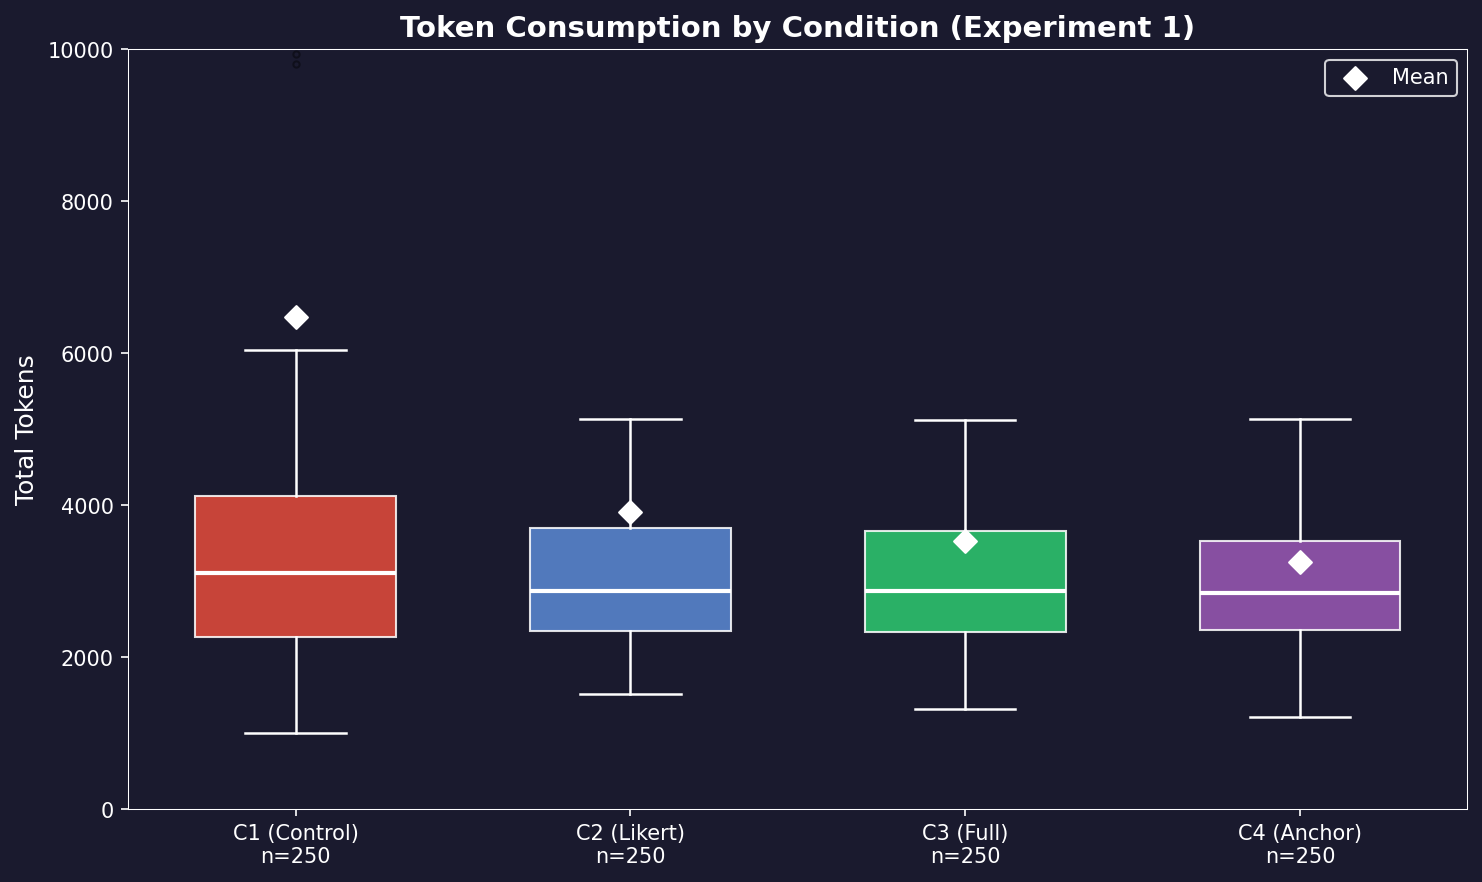
\includegraphics[width=\columnwidth]{../results/figures/fig1_v2_token_boxplot.png}
\caption{Token consumption distributions by condition (v2). The heavy right tail of C1 reflects multi-step episodes (11.6\% of tasks), which are progressively eliminated in treatment conditions. The treatment effect operates primarily through tail compression rather than location shift.}
\label{fig:v2_token_boxplot}
\end{figure}

\subsection{Bandit Convergence}
\label{sec:convergence}

Thompson Sampling produces distinct convergence patterns across conditions.

\textbf{C2 (Likert feedback)} converges to the importance-heavy preset (posterior mean 0.633 by the final quartile), with the balanced preset (Park et al.\ default) ranking near the bottom.
\textbf{C3 (Likert + explanation embeddings)} converges to the relevance-importance preset (0.616) and converges faster than C2 (by Q2 vs.\ Q3), with wider posterior spread (0.151 vs.\ 0.106).
The explanation embeddings stored in C3 appear to strengthen the reward signal.
\textbf{C4 (qualitative anchors)} shows no convergence: all arms hover near 0.42 (spread $=$0.014).
Despite achieving the best token efficiency, C4's anchor embedding parser compresses reward variance 3.6$\times$ relative to Likert parsing, leaving insufficient signal for the bandit to differentiate arms.

The C4 paradox, best efficiency with no weight learning, is the key diagnostic finding.
It demonstrates that the token efficiency gains in Experiment~1 are driven by the \emph{rubric prompt effect} (present in all treatment conditions), not by the \emph{adaptive retrieval effect} (present only when the bandit converges).
This has three implications: (1)~the rubric prompt effect is \emph{largely independent of} retrieval weight adaptation, providing its benefit independently of whether the bandit converges; (2)~embedding-based reward inference (C4's anchor parser) trades off signal fidelity for ecological validity: the 3.6$\times$ variance compression produces smoother but less informative rewards; (3)~future work on adaptive retrieval must control for the rubric prompt confound, isolating weight learning effects from metacognitive anchoring effects.

\subsection{Diagnosis: Why Weight Learning Didn't Improve Retrieval}

\paragraph{Skill overlap.}
Pairwise Jaccard similarity of the top-5 retrieved skills between conditions: C1 vs.\ C2 $= 0.904$, C1 vs.\ C3 $= 0.909$, C1 vs.\ C4 $= 0.848$.
Different weight presets change the \emph{scores} of skills but not the \emph{rankings}: the same ${\sim}$6 meta-skills dominate 86\% of all retrievals regardless of weights (Appendix Figure~\ref{fig:skill_heatmap}).

\paragraph{Root cause: dimension saturation.}
The recency dimension is near-saturated at ${\sim}$0.95 (most skills were used recently in a sequential experiment) and importance at ${\sim}$0.96 (Laplace smoothing with high success rate).
Only relevance (${\sim}$0.43) has meaningful variance (see Figure~\ref{fig:v3_jaccard_trajectory} for the trajectory across both experiments).
With two of three dimensions effectively constant, weight changes cannot produce different skill orderings.

\paragraph{Two independent effects.}
We identify two separable mechanisms:
\begin{enumerate}
\item \textbf{Rubric prompt effect} (all treatment conditions): The feedback rubric structures the LLM's response, preventing multi-step spirals. This is a prompt engineering effect, not a retrieval effect.
\item \textbf{Adaptive retrieval effect} (C2/C3 only): Thompson Sampling converges, but convergence does not change retrieved skills due to dimension saturation.
\end{enumerate}
C4 achieves effect~1 without effect~2's overhead, explaining its paradoxical advantage.

\paragraph{Per-difficulty breakdown.}
The rubric prompt effect scales with task difficulty: easy tasks show 6--15\% token reduction, medium tasks 30--45\%, and hard tasks 60--70\%.
This is consistent with the multi-step prevention mechanism: harder tasks are more likely to trigger reasoning spirals, so preventing those spirals yields larger savings.


\section{Experiment 2: Expanded Library (v3)}
\label{sec:experiment_v3}
% Section 5: Experiment 2 — Expanded Library (v3) (~2.5 pages)

\subsection{Design Rationale}

Experiment~1 diagnosed three design flaws that prevented weight learning from improving retrieval:
(a)~too few skills (50), causing a small number of generic meta-skills to dominate;
(b)~skills too domain-general, making all skills roughly equally relevant to any task;
(c)~recency and importance dimensions near-saturated (${\sim}$0.95), leaving only relevance with meaningful variance.
Experiment~1 also used \texttt{max\_tokens}$=$4{,}096, which introduced truncation cascades: every non-final step hit the output limit, causing the runner to continue iterating with accumulated context.
This confound inflated multi-step rates and made it impossible to distinguish genuine behavioral effects from truncation artifacts.

Experiment~2 addresses all four issues:
\begin{itemize}
\item \textbf{205 domain-specific skills:} 30 base skills plus 175 specialized skills (${\sim}$35 per theme), ensuring that topic-specific tasks have enough candidate skills for weight differences to change rankings.
\item \textbf{12 weight presets:} The original 5 plus 7 new presets including extreme configurations (85/5/10) and an anti-relevance preset (45/45/10) that explicitly tests whether de-emphasizing semantic similarity helps for certain task types.
\item \textbf{300 harder tasks:} 50 easy, 100 medium, 150 hard, shifting the distribution toward tasks where retrieval quality should matter most.
\item \textbf{\texttt{max\_tokens}$=$16{,}384:} Eliminates truncation cascades by ensuring the LLM can always complete its response in a single generation.
\end{itemize}

\paragraph{Key predictions.}
If the fix works: (1)~Jaccard overlap between conditions should drop from $>$0.90 to $<$0.60; (2)~bandit convergence in C2/C3 should correlate with improved ground truth hit rate; (3)~C4 should either develop convergence (if the anchor parser produces enough variance with 12 arms) or remain the ``rubric-only'' baseline.

\subsection{Results}

\begin{table}[t]
\centering
\small
\begin{tabular}{lrrrrrr}
\toprule
\textbf{Cond.} & \textbf{Mean Tok.} & \textbf{Med.} & \textbf{SD} & \textbf{$\Delta$C1} & \textbf{NDCG@5} & \textbf{Jacc.} \\
\midrule
C1 & 5{,}517 & 4{,}910 & 2{,}449 & --- & 0.371 & --- \\
C2 & 4{,}824 & 4{,}204 & 1{,}896 & $-$12.6\% & 0.394 & 0.585 \\
C3 & 4{,}830 & 4{,}286 & 1{,}820 & $-$12.5\% & 0.469 & 0.517 \\
C4 & 4{,}429 & 4{,}100 & 1{,}429 & $-$19.7\% & 0.374 & 0.573 \\
\bottomrule
\end{tabular}
\caption{Experiment~2 main results ($N{=}300$ per condition, 1{,}200 total episodes). Token reduction is relative to C1 mean. Jaccard reports mean per-episode overlap of top-5 retrieved skill sets against C1. Only 1 of 1{,}200 episodes triggered multi-step reasoning. Kruskal--Wallis $H(3){=}33.87$, $p{<}0.001$. All three C1-vs-treatment comparisons survive Holm--Bonferroni correction ($p{<}0.001$).}
\label{tab:v3_results}
\end{table}

\paragraph{Token efficiency.}
Table~\ref{tab:v3_results} summarizes the main results.
All three feedback conditions reduce mean token consumption by 12--20\% relative to C1, with C4 achieving the largest reduction ($-$19.7\%).
The Kruskal--Wallis test confirms that the four conditions differ significantly ($H(3){=}33.87$, $p{<}0.001$).
After Holm--Bonferroni correction for six pairwise comparisons, all three C1-vs-treatment comparisons remain significant: C1 vs.\ C4 ($p{<}0.001$, $d{=}0.543$), C1 vs.\ C2 ($p{=}0.0003$, $d{=}0.317$), and C1 vs.\ C3 ($p{=}0.0004$, $d{=}0.319$).
Treatment-vs-treatment comparisons are not significant after correction.
BCa bootstrap 95\% CIs for the mean difference (10{,}000 resamples) are C1$-$C2: $[340,\, 1{,}052]$, C1$-$C3: $[341,\, 1{,}033]$, C1$-$C4: $[772,\, 1{,}418]$; all exclude zero (Figure~\ref{fig:v3_token_boxplot}).

\begin{figure}[t]
\centering
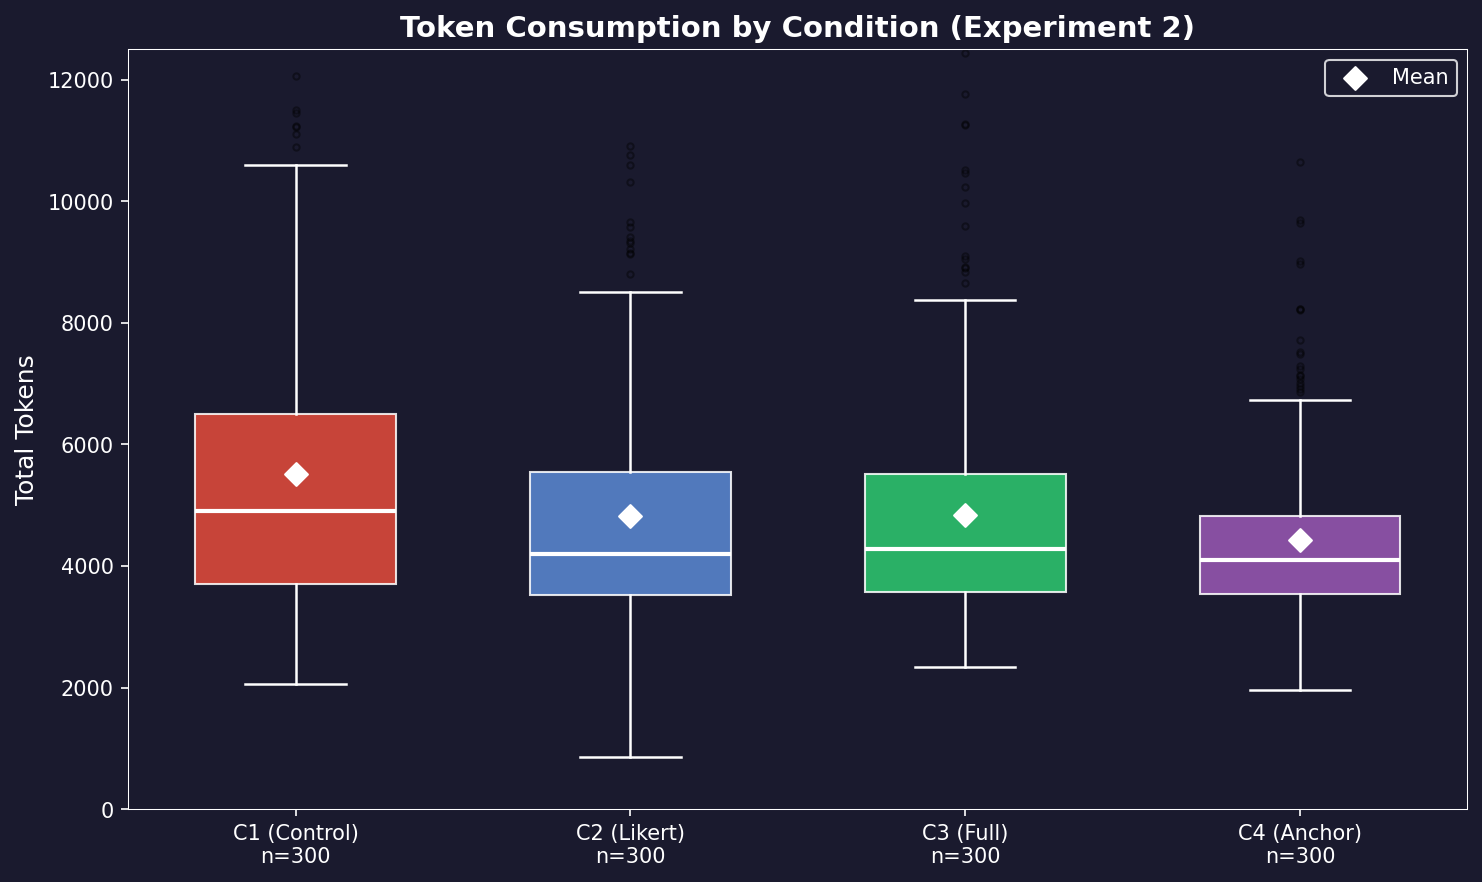
\includegraphics[width=\columnwidth]{../results/figures/fig1_v3_token_boxplot.png}
\caption{Token consumption distributions by condition (v3). With truncation cascades eliminated (\texttt{max\_tokens}$=$16{,}384), all conditions produce unimodal distributions with moderate right skew. The treatment effect is visible as a shift in both location and spread: C4 SD${=}$1{,}429 vs.\ C1 SD${=}$2{,}449.}
\label{fig:v3_token_boxplot}
\end{figure}

\paragraph{Output-driven mechanism.}
Unlike Experiment~1, where the treatment effect was driven by multi-step prevention (a truncation artifact), Experiment~2 reveals the underlying mechanism: feedback conditions produce \emph{shorter LLM outputs}.
Only 1 of 1{,}200 episodes triggered multi-step reasoning (C1, task~023, 2 steps, 21{,}259 tokens), effectively eliminating multi-step behavior as an explanatory variable.
Instead, the token reduction is concentrated in output tokens: C1 generates a mean of 3{,}813 output tokens per episode, compared to 2{,}960 (C2, $-$22\%), 2{,}946 (C3, $-$23\%), and 2{,}537 (C4, $-$33\%).
Input tokens are comparable across conditions (${\sim}$1{,}700--1{,}890), confirming that the difference lies in generation length, not prompt construction.

This suggests two separable effects: improved retrieval quality from weight learning, and the structured rubric prompt producing more focused output.
The rubric's metacognitive scaffolding appears to reduce verbose exploration in the LLM's output independently of which skills were retrieved, an effect that operates through prompt structure rather than retrieval architecture.

\paragraph{Input/output token split.}
C1 episodes are 69\% output tokens (0.45:1 input-to-output ratio), while feedback conditions shift toward higher input proportions: C2 61\% output (0.63:1), C3 61\% (0.64:1), C4 57\% (0.75:1).
The increasing input-to-output ratio from C1 to C4 is consistent with the rubric adding structured input tokens while the LLM produces proportionally shorter outputs (Figure~\ref{fig:v3_io_tokens}).

\begin{figure}[t]
\centering
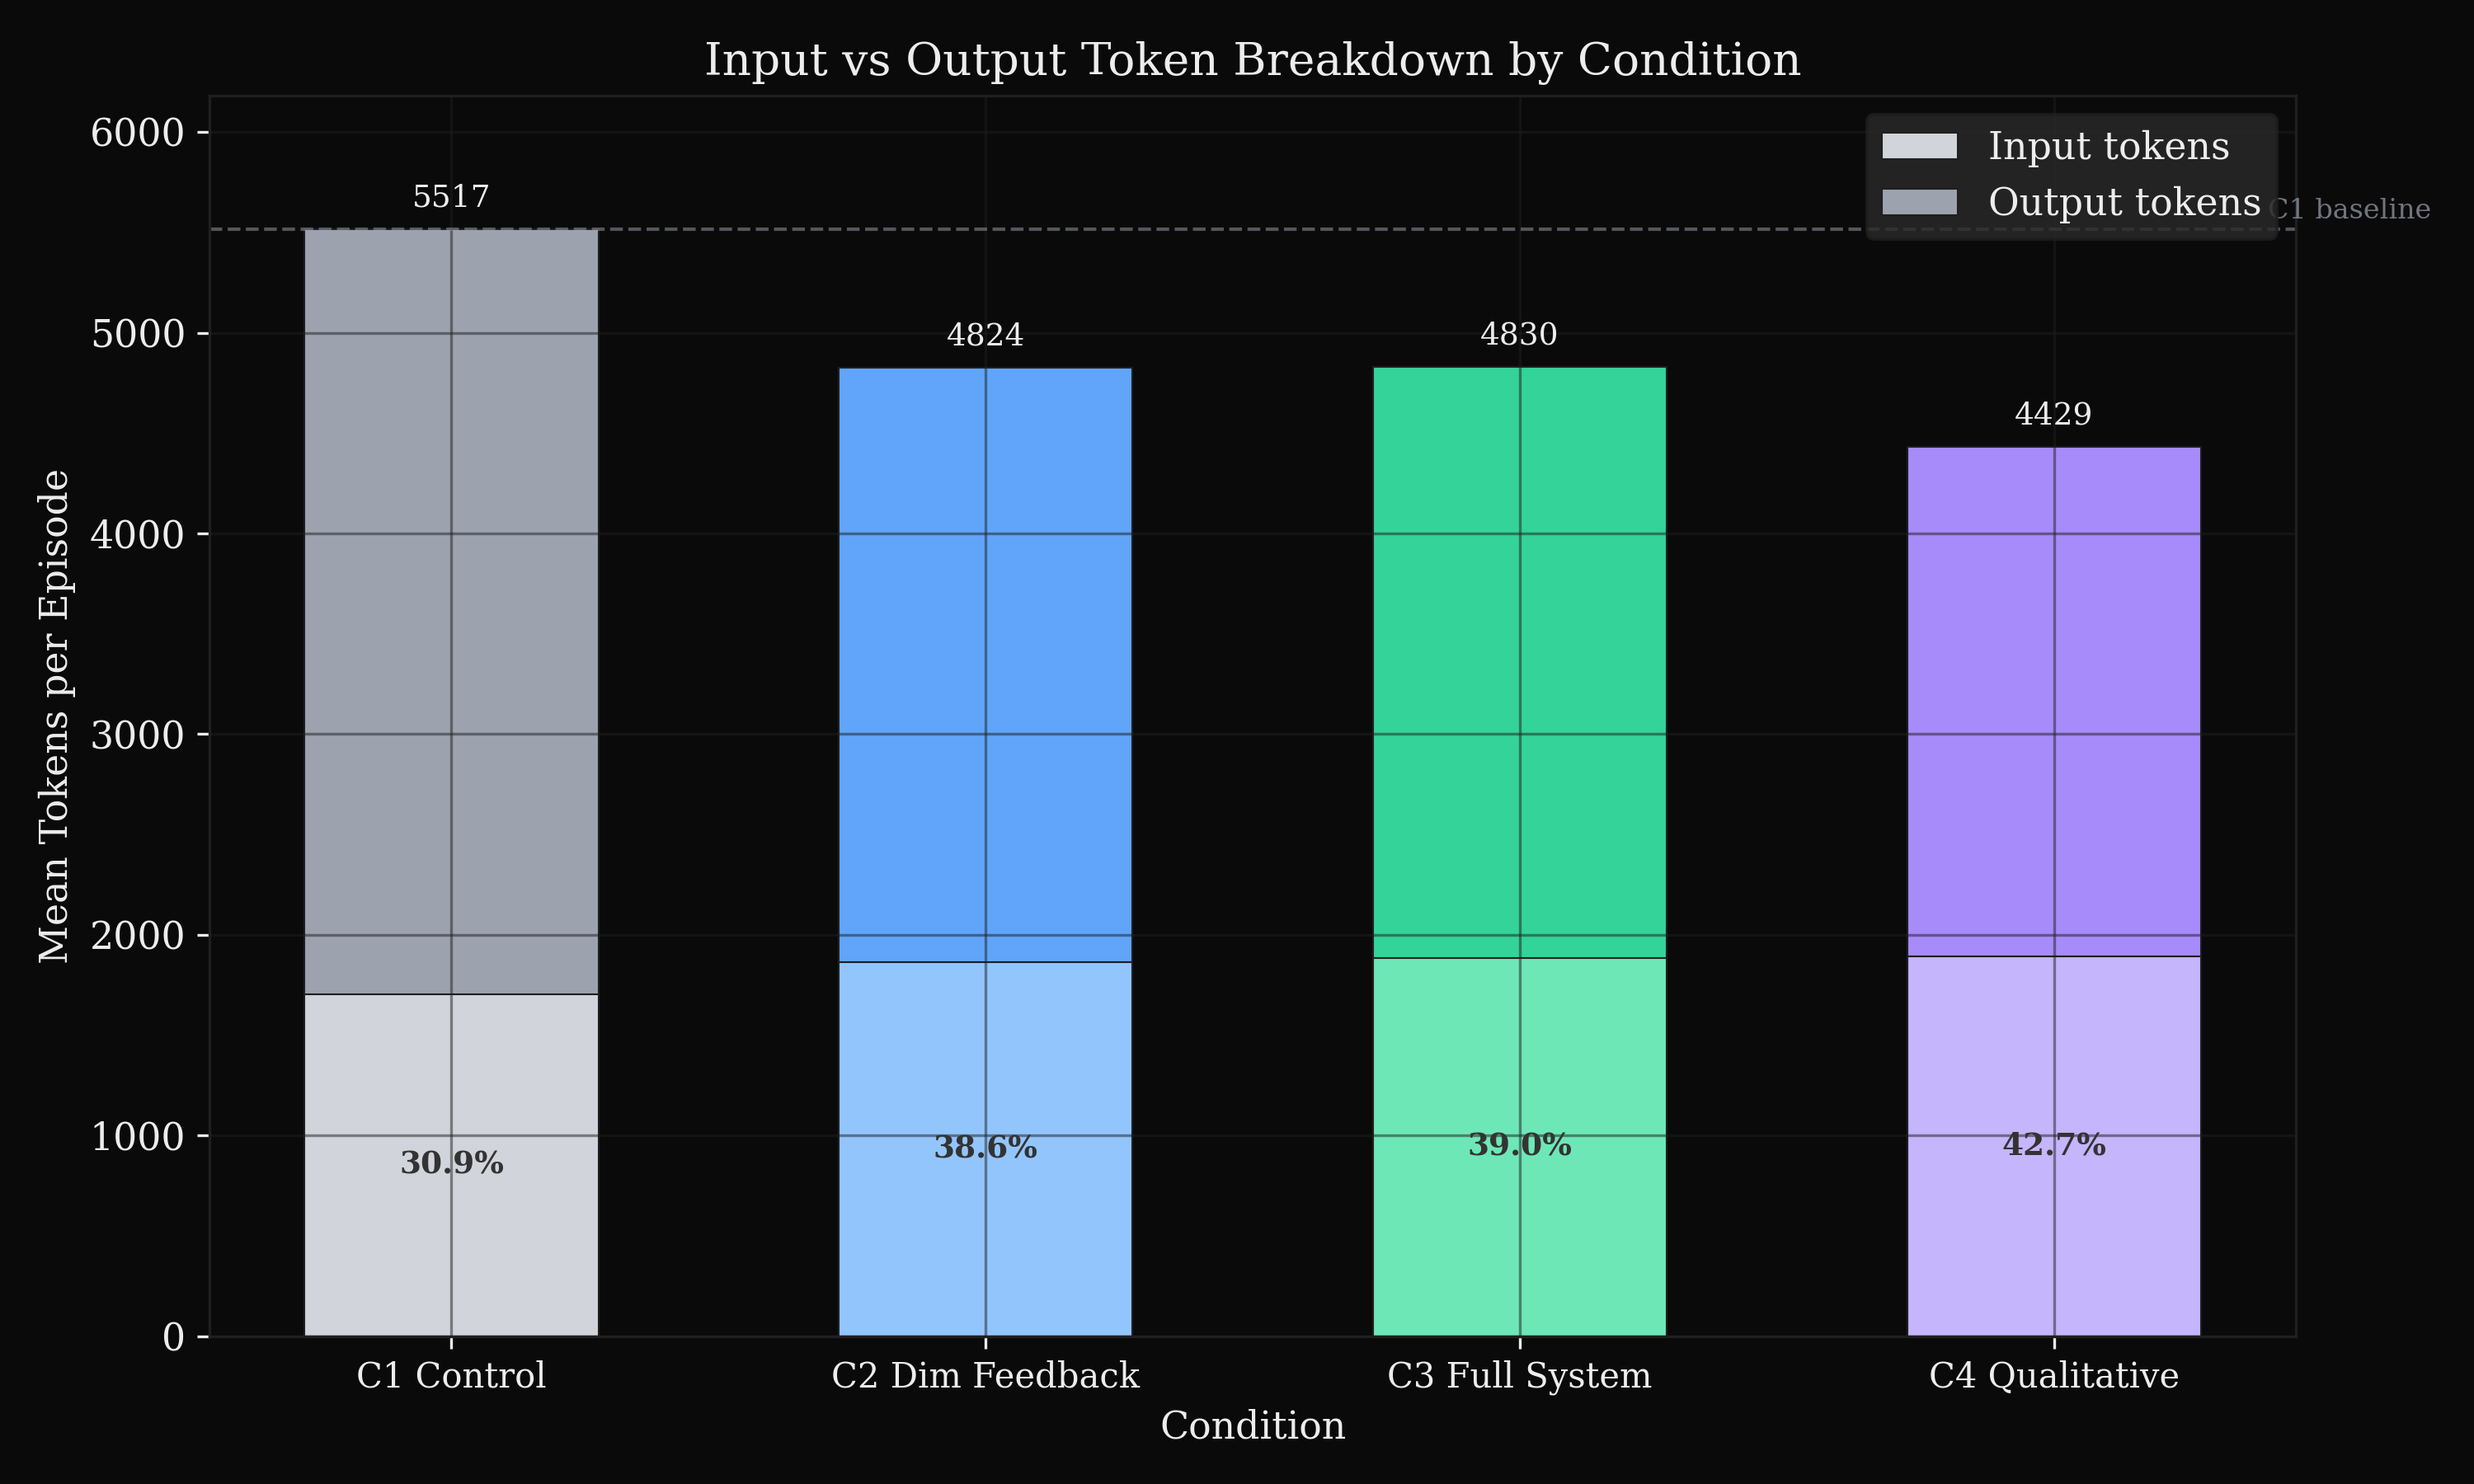
\includegraphics[width=\columnwidth]{../results/figures/figIO1_stacked_bar_tokens.png}
\caption{Input vs.\ output token breakdown by condition (v3). The treatment effect is concentrated in output tokens: C4 produces 33\% fewer output tokens than C1, while input tokens are comparable across conditions (${\sim}$1{,}700--1{,}890). The increasing input-to-output ratio from C1 (0.45:1) to C4 (0.75:1) reflects the rubric adding structured input while the LLM generates proportionally shorter outputs.}
\label{fig:v3_io_tokens}
\end{figure}

\paragraph{Temporal trend.}
C1 shows stable token consumption across the experiment (first half: 5{,}564, second half: 5{,}471, $-$1.7\%).
C2 shows a modest learning effect: 5{,}055$\,\rightarrow\,$4{,}594 ($-$9.1\%), consistent with the bandit gradually improving its weight selection.
C3 ($-$1.9\%) and C4 ($+$0.8\%) are essentially stable, suggesting that C3's retrieval quality improvements do not translate into further token savings once the rubric effect is accounted for, and C4's anchor-based feedback does not produce a detectable learning trajectory on this metric.

\subsection{Retrieval Differentiation}

The central question of Experiment~2 is whether the expanded library and de-saturated dimensions enable weight learning to genuinely change retrieved skills.

\paragraph{Jaccard overlap.}

\begin{figure}[t]
\centering
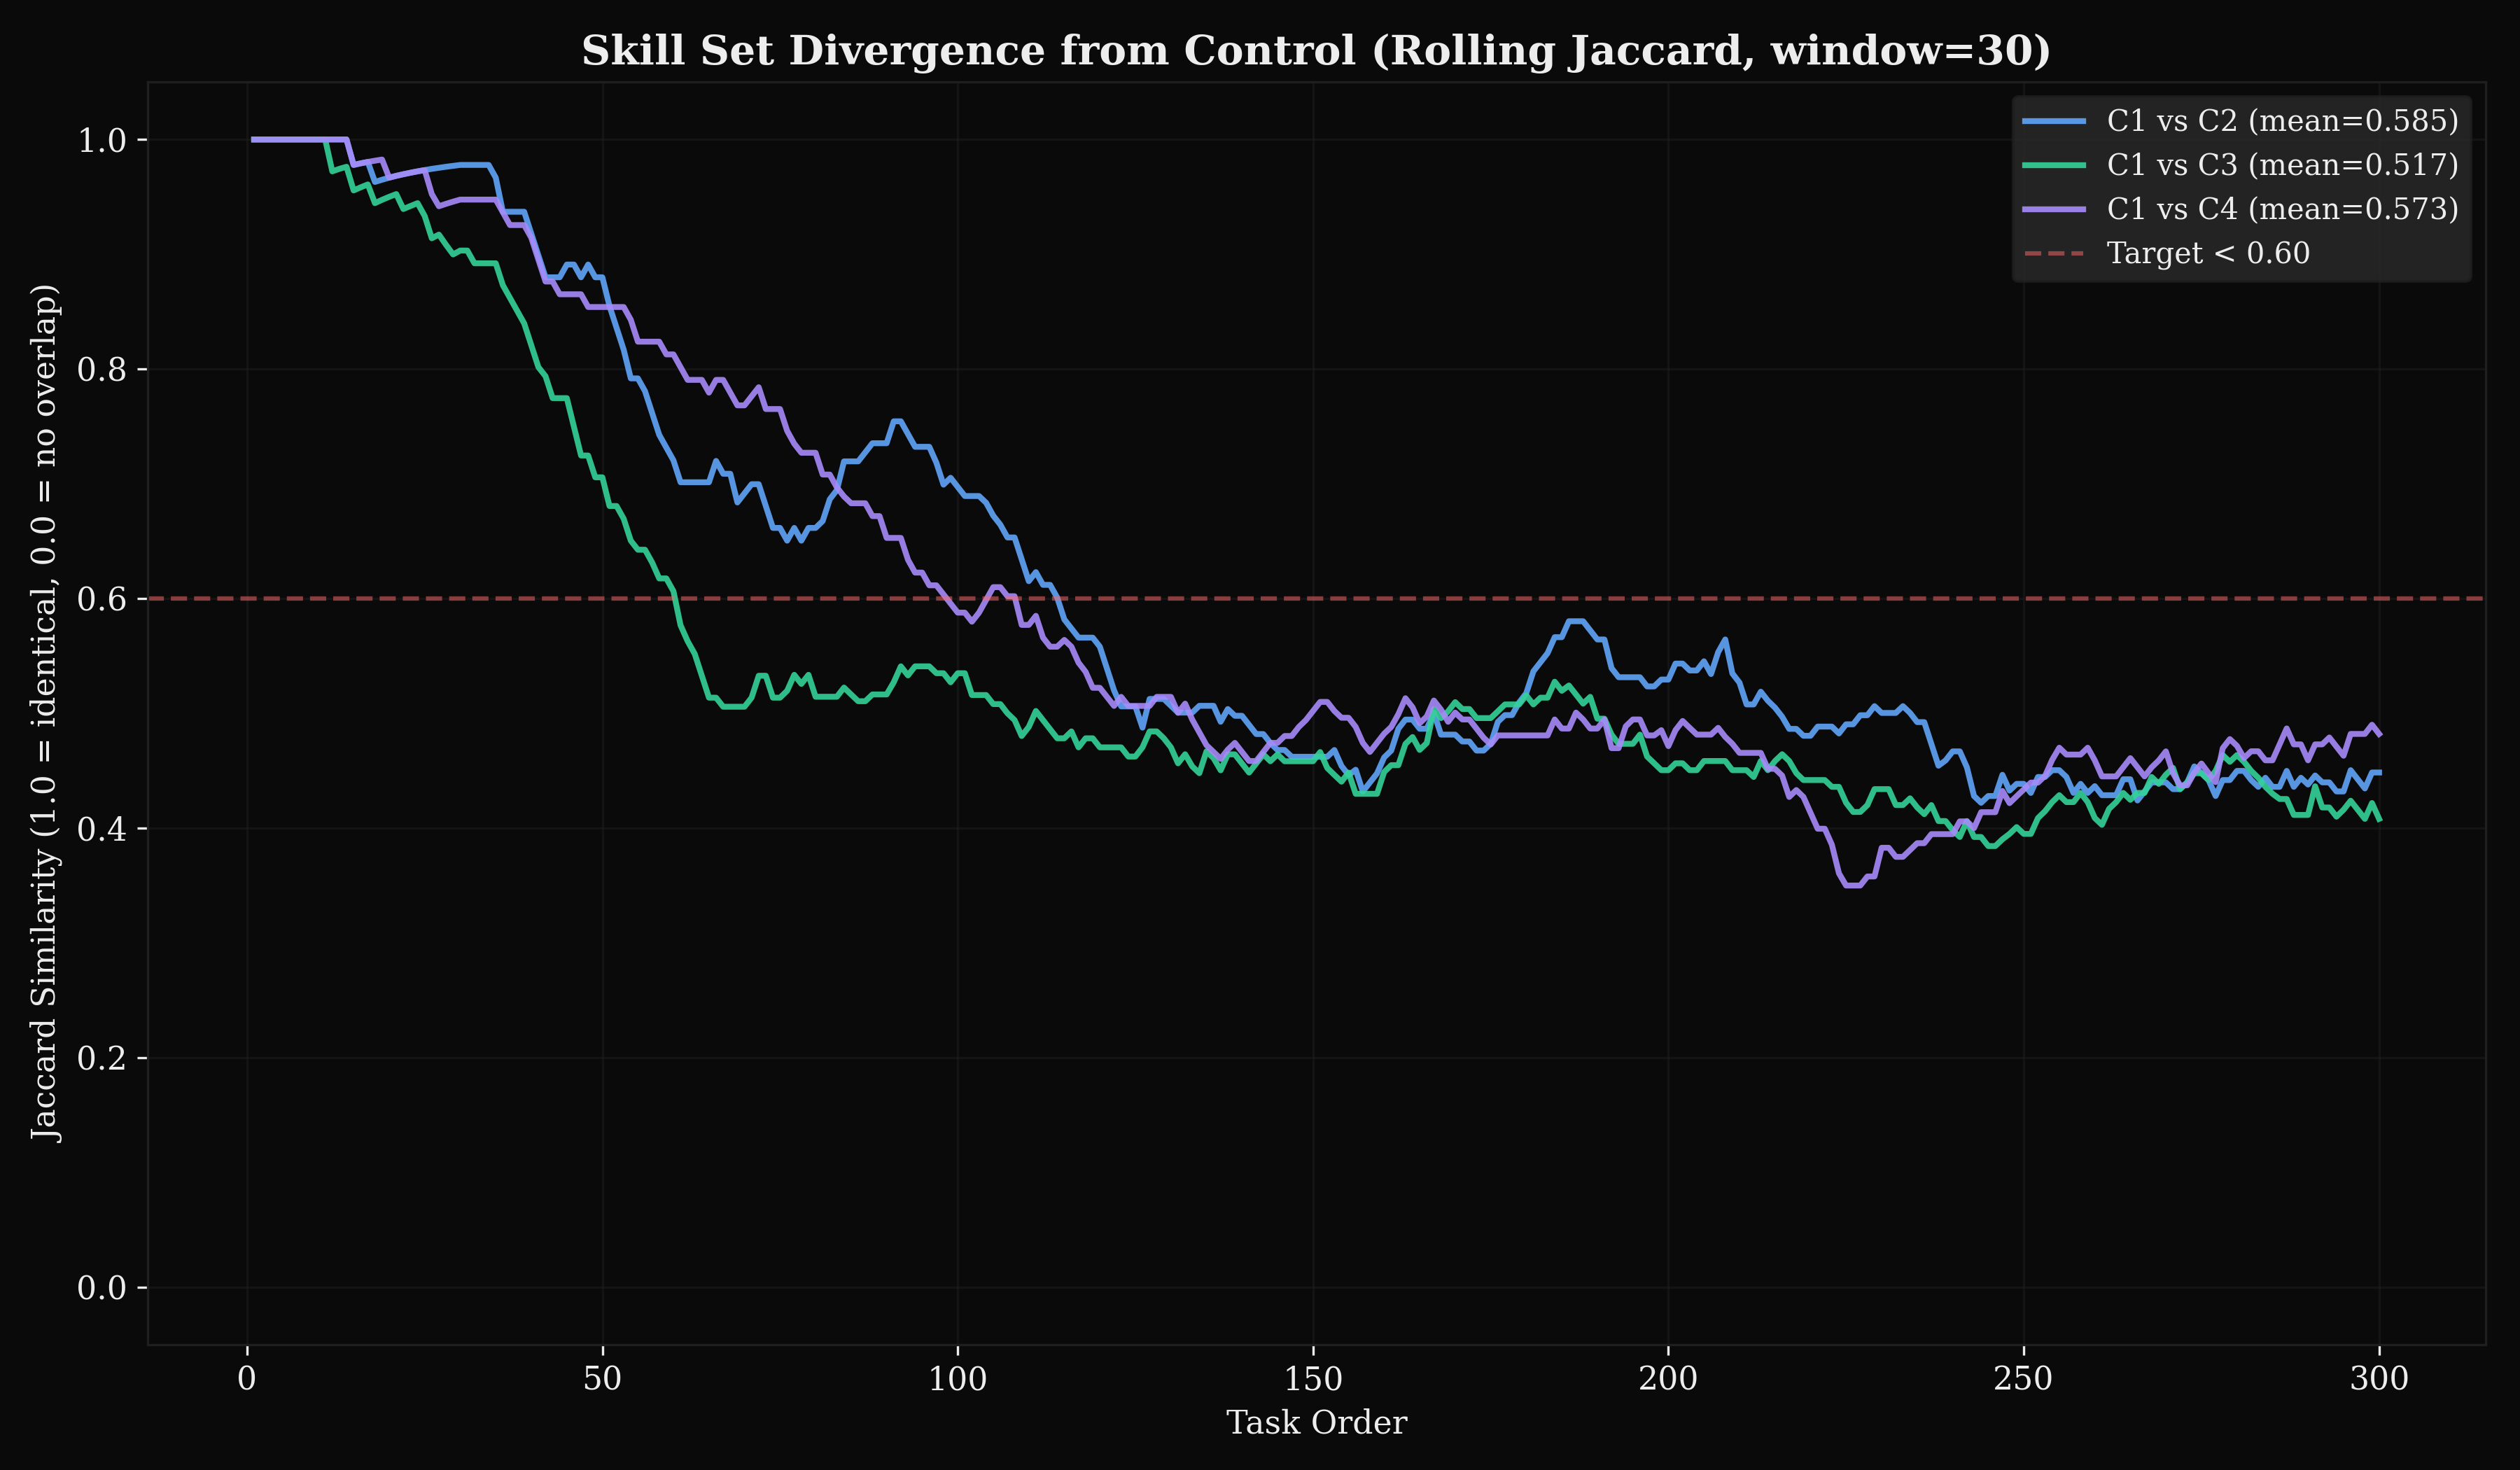
\includegraphics[width=\columnwidth]{../results/figures/fig7_jaccard_trajectory.png}
\caption{Pairwise Jaccard similarity of top-5 retrieved skills over episodes. In v2, all C1-vs-treatment pairs were above 0.84, indicating near-identical retrievals regardless of weight configuration. In v3, C1-vs-treatment pairs drop to 0.52--0.59, meeting the \emph{a priori} $<$0.60 threshold and confirming that weight learning now produces meaningfully different skill sets.}
\label{fig:v3_jaccard_trajectory}
\end{figure}

Mean per-episode Jaccard drops from $>$0.90 (v2) to 0.585 (C1 vs.\ C2), 0.517 (C1 vs.\ C3), and 0.573 (C1 vs.\ C4).
All three C1-vs-treatment values are at or below the 0.60 threshold set \emph{a priori}, confirming that different weight configurations now retrieve meaningfully different skill sets (Table~\ref{tab:v3_results}, Figure~\ref{fig:v3_jaccard_trajectory}).
C3 achieves the lowest overlap with C1 (0.517), consistent with its stronger bandit convergence driving more distinctive weight selections.
The reduction from v2 (0.90$\,\rightarrow\,$0.52--0.59) represents a ${\sim}$37\% decrease in retrieval overlap.

\paragraph{Unique skill usage.}
All conditions use the expanded library broadly: C1 uses 158 unique skills, C2 uses 169, C3 uses 163, and C4 uses 151.
Unlike v2, where C1 was restricted to 5 generic meta-skills, the expanded library ensures that even the control condition accesses diverse skills.
The differentiation between conditions is therefore not in \emph{which} skills are accessible, but in \emph{how they are ranked}, precisely the mechanism that weight learning targets.

\paragraph{Ground truth hit rate.}
Each task has 1--3 annotated ground truth skills.
C1 achieves a 59.7\% hit rate (at least one ground truth skill in the top-5), compared to 59.3\% for C2, 67.3\% for C3, and 58.0\% for C4 (Figure~\ref{fig:v3_gt_hit_rate}).
The rank-aware retrieval metrics show a clearer separation: NDCG@5 is 0.371 (C1), 0.394 (C2), 0.469 (C3), 0.374 (C4); MRR is 0.302 (C1), 0.331 (C2), 0.411 (C3), 0.313 (C4).
C3 achieves the best retrieval quality across all metrics, with NDCG@5 $+$26.3\% and MRR $+$35.9\% relative to C1 (descriptive comparisons; formal significance tests were not conducted for rank-aware retrieval metrics).
This suggests that the explanation embedding pipeline produces a higher-quality reward signal that enables more effective weight learning.

\begin{figure}[t]
\centering
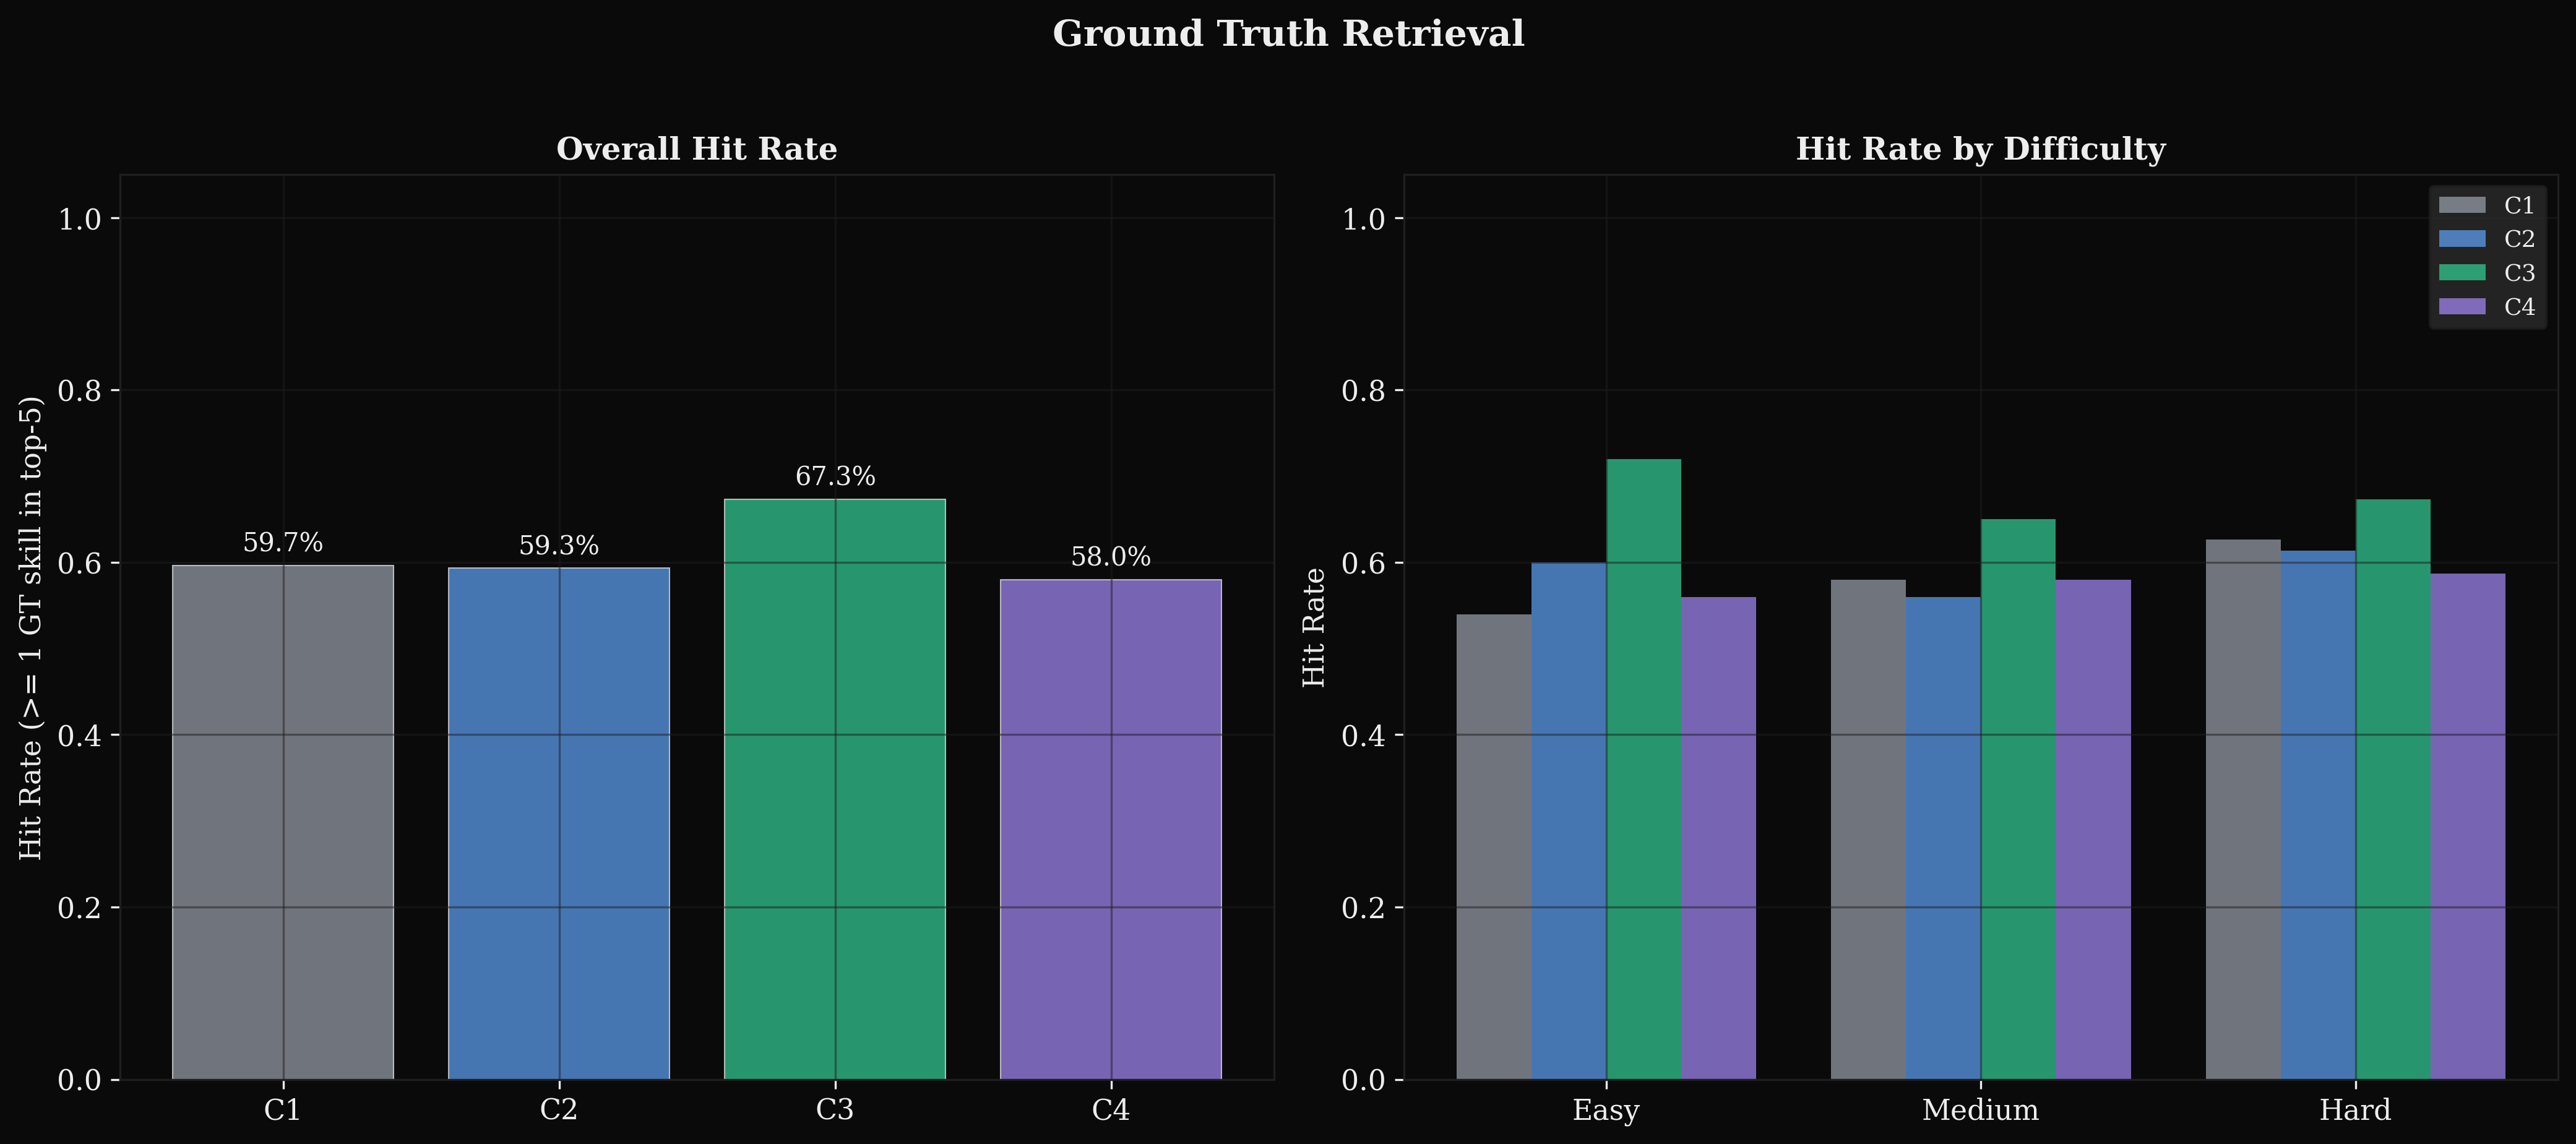
\includegraphics[width=\columnwidth]{../results/figures/fig6_ground_truth_hit_rate.png}
\caption{Retrieval quality by condition (v3). C3 (Full System) achieves the highest NDCG@5 and MRR, consistent with explanation embeddings producing a higher-fidelity reward signal for Thompson Sampling. The improvement is concentrated in ranking quality (NDCG, MRR) rather than binary hit rate, suggesting that weight learning improves skill \emph{ordering} more than skill \emph{selection}.}
\label{fig:v3_gt_hit_rate}
\end{figure}

\subsection{Bandit Convergence}
\label{sec:v3_convergence}

With 12 arms and 300 episodes, Thompson Sampling exhibits three qualitatively distinct convergence patterns (Figure~\ref{fig:v3_bandit_posteriors}).

\textbf{C2 (Likert feedback)} converges to \texttt{pure\_relevance} ($E[\theta]{=}0.709$, 41 pulls), with \texttt{recency\_heavy} as the second-most-pulled arm (50 pulls, $E[\theta]{=}0.704$).
This is a notable shift from Experiment~1, where C2 converged to the importance-heavy preset.
With de-saturated dimensions and specialized skills, the Likert reward signal correctly identifies that semantic relevance is the most informative dimension for retrieval in this library.

\textbf{C3 (Full System)} converges more decisively to \texttt{pure\_relevance} ($E[\theta]{=}0.749$, 73 pulls), with the widest gap over the second arm (\texttt{relevance\_heavy}, $E[\theta]{=}0.719$).
C3's stronger convergence, both higher posterior mean and more concentrated pulls, suggests that the explanation embedding pipeline produces a higher signal-to-noise reward than C2's Likert scores.
The bandit reaches a stable selection pattern by approximately task 33--48, after which \texttt{pure\_relevance} dominates the selection distribution.

\textbf{C4 (Qualitative anchors)} converges weakly to \texttt{pure\_importance} ($E[\theta]{=}0.472$, 35 pulls), with the remaining arms clustered between 0.440 and 0.455.
Unlike the v2 finding of completely flat posteriors, C4 does exhibit a preference, but the compressed posterior range (0.440--0.472) indicates that the anchor parser's reward signal has insufficient variance to drive strong differentiation.

\begin{figure}[t]
\centering
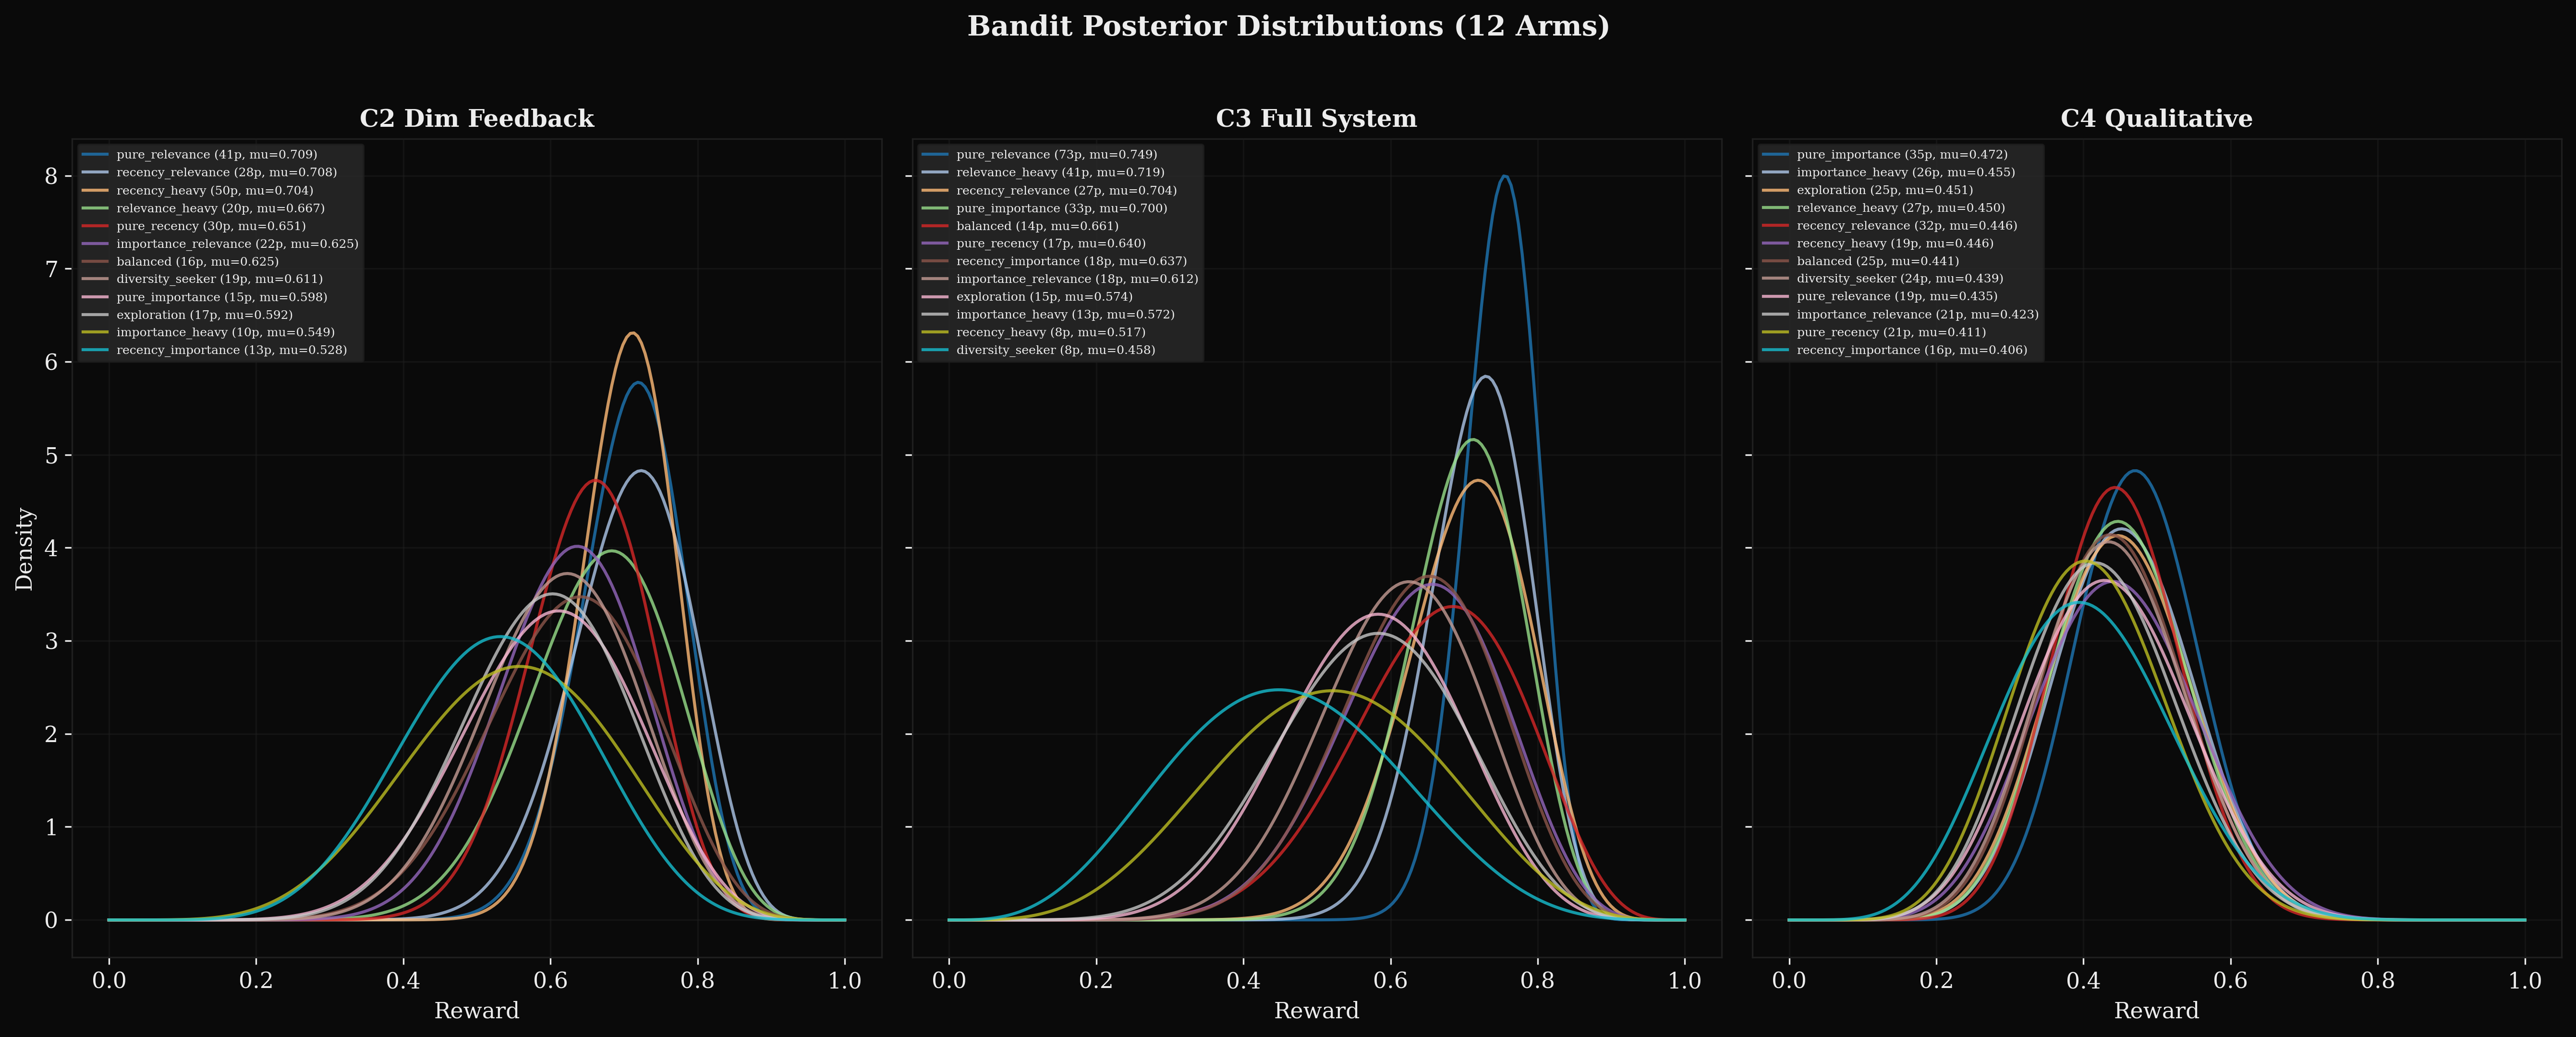
\includegraphics[width=\columnwidth]{../results/figures/figA7_bandit_posteriors.png}
\caption{Thompson Sampling posterior means over episodes (v3, 12 arms). C2 and C3 converge to \texttt{pure\_relevance}, confirming that semantic relevance is the most informative retrieval dimension when the skill library provides sufficient diversity. C4 converges weakly to \texttt{pure\_importance}, with compressed posteriors reflecting the anchor parser's limited discriminative signal.}
\label{fig:v3_bandit_posteriors}
\end{figure}

\paragraph{C4 anchor spread.}
The C4 anchor parser produces per-dimension scores of recency mean${=}$0.14 (SD${=}$0.07), importance mean${=}$0.62 (SD${=}$0.17), relevance mean${=}$0.55 (SD${=}$0.13).
The recency dimension is effectively dead: the ``high recency'' anchor text describes an extreme that typical LLM responses rarely approach, causing the softmax projection to consistently assign low recency scores.
This compressed recency signal explains C4's convergence to \texttt{pure\_importance} rather than \texttt{pure\_relevance}: the bandit optimizes over the dimensions with usable variance.
Parse rates are high across conditions (C2: 93.7\%, C3: 95.0\%, C4: 96.7\%), confirming that C4's weaker convergence is a signal fidelity issue, not a parsing failure.

\subsection{Analysis}

\paragraph{Per-difficulty breakdown.}
The output-driven efficiency effect scales with task difficulty.
Easy tasks: C1${=}$3{,}995, C4${=}$3{,}523 ($-$12\%).
Medium tasks: C1${=}$5{,}573, C4${=}$4{,}409 ($-$21\%).
Hard tasks: C1${=}$5{,}987, C4${=}$4{,}745 ($-$21\%).
All difficulty levels show reductions, but the effect is larger for medium and hard tasks, where C1 generates longer outputs (mean output: easy${=}$2{,}295, medium${=}$3{,}883, hard${=}$4{,}273).
The rubric's metacognitive scaffolding appears most effective when the LLM faces complex tasks that would otherwise produce verbose, exploratory responses (Figure~\ref{fig:v3_difficulty}).

\begin{figure}[t]
\centering
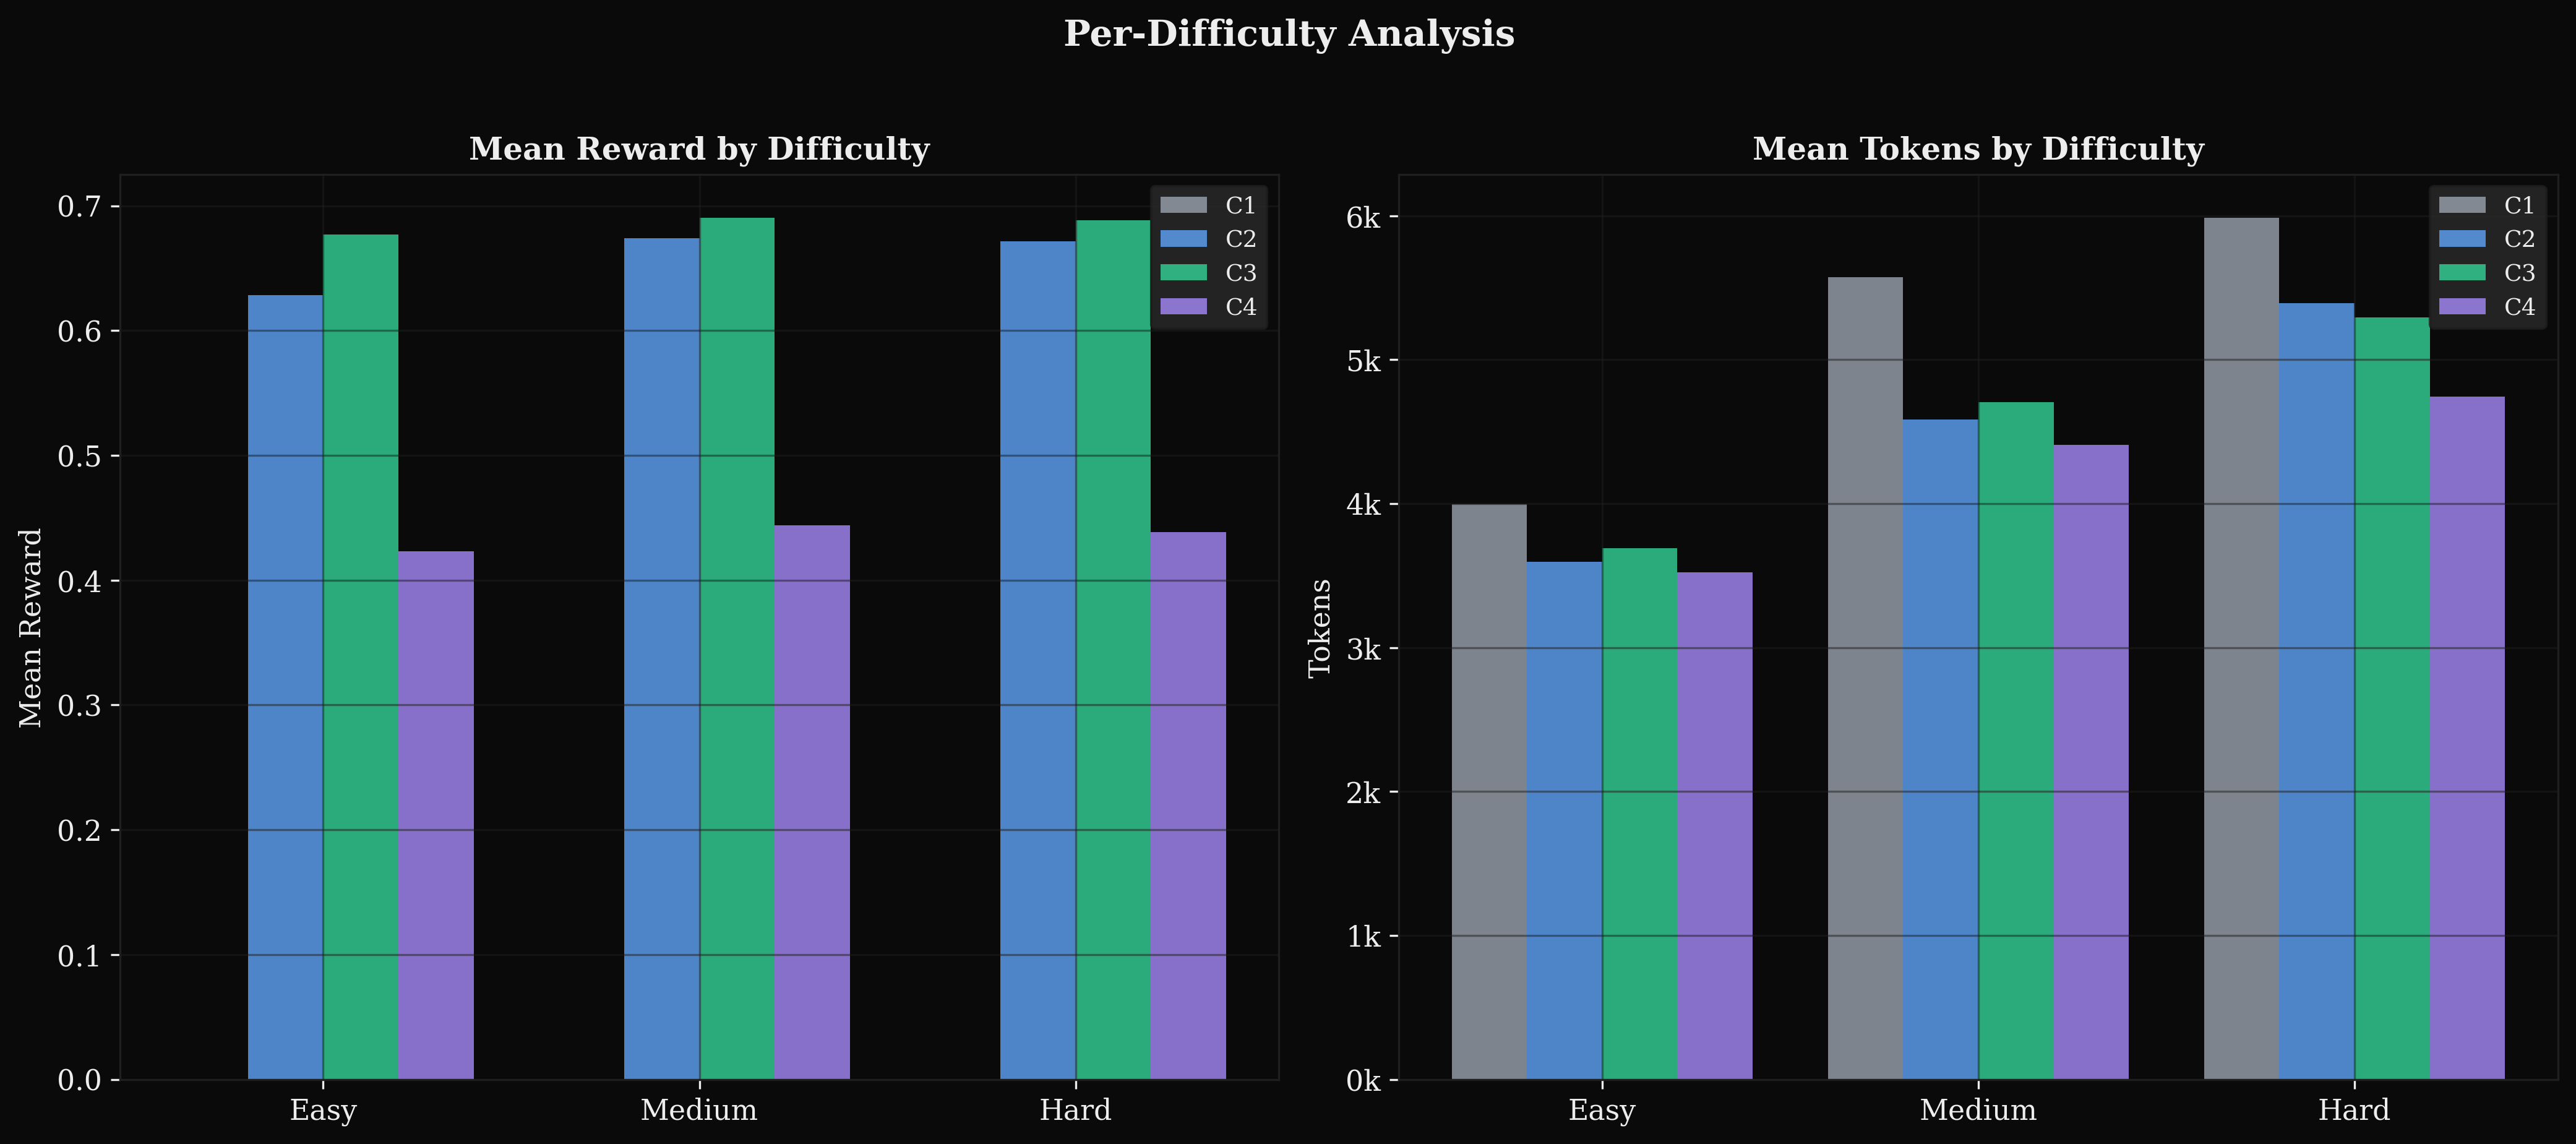
\includegraphics[width=\columnwidth]{../results/figures/figA8_difficulty_comparison.png}
\caption{Mean token consumption by difficulty level and condition (v3). The treatment effect scales with difficulty: $-$12\% for easy, $-$21\% for medium and hard tasks. Unlike Experiment~1 (where easy tasks showed rubric overhead), all difficulty levels benefit from the treatment in Experiment~2.}
\label{fig:v3_difficulty}
\end{figure}

\paragraph{Per-theme breakdown.}
The treatment effect varies across themes.
The largest reductions appear in retrieval\_systems (C1${=}$6{,}385, C4${=}$4{,}583, $-$28\%) and ml\_fundamentals (C1${=}$5{,}011, C4${=}$3{,}877, $-$23\%).
Themes where C1 generates the longest outputs benefit most from the rubric's output-constraining effect.
The smallest reduction is in evaluation\_methods (C1${=}$5{,}274, C4${=}$4{,}650, $-$12\%), possibly because evaluation tasks naturally produce more structured, concise responses even without rubric guidance (Figure~\ref{fig:v3_domain_heatmap}).

\begin{figure}[t]
\centering
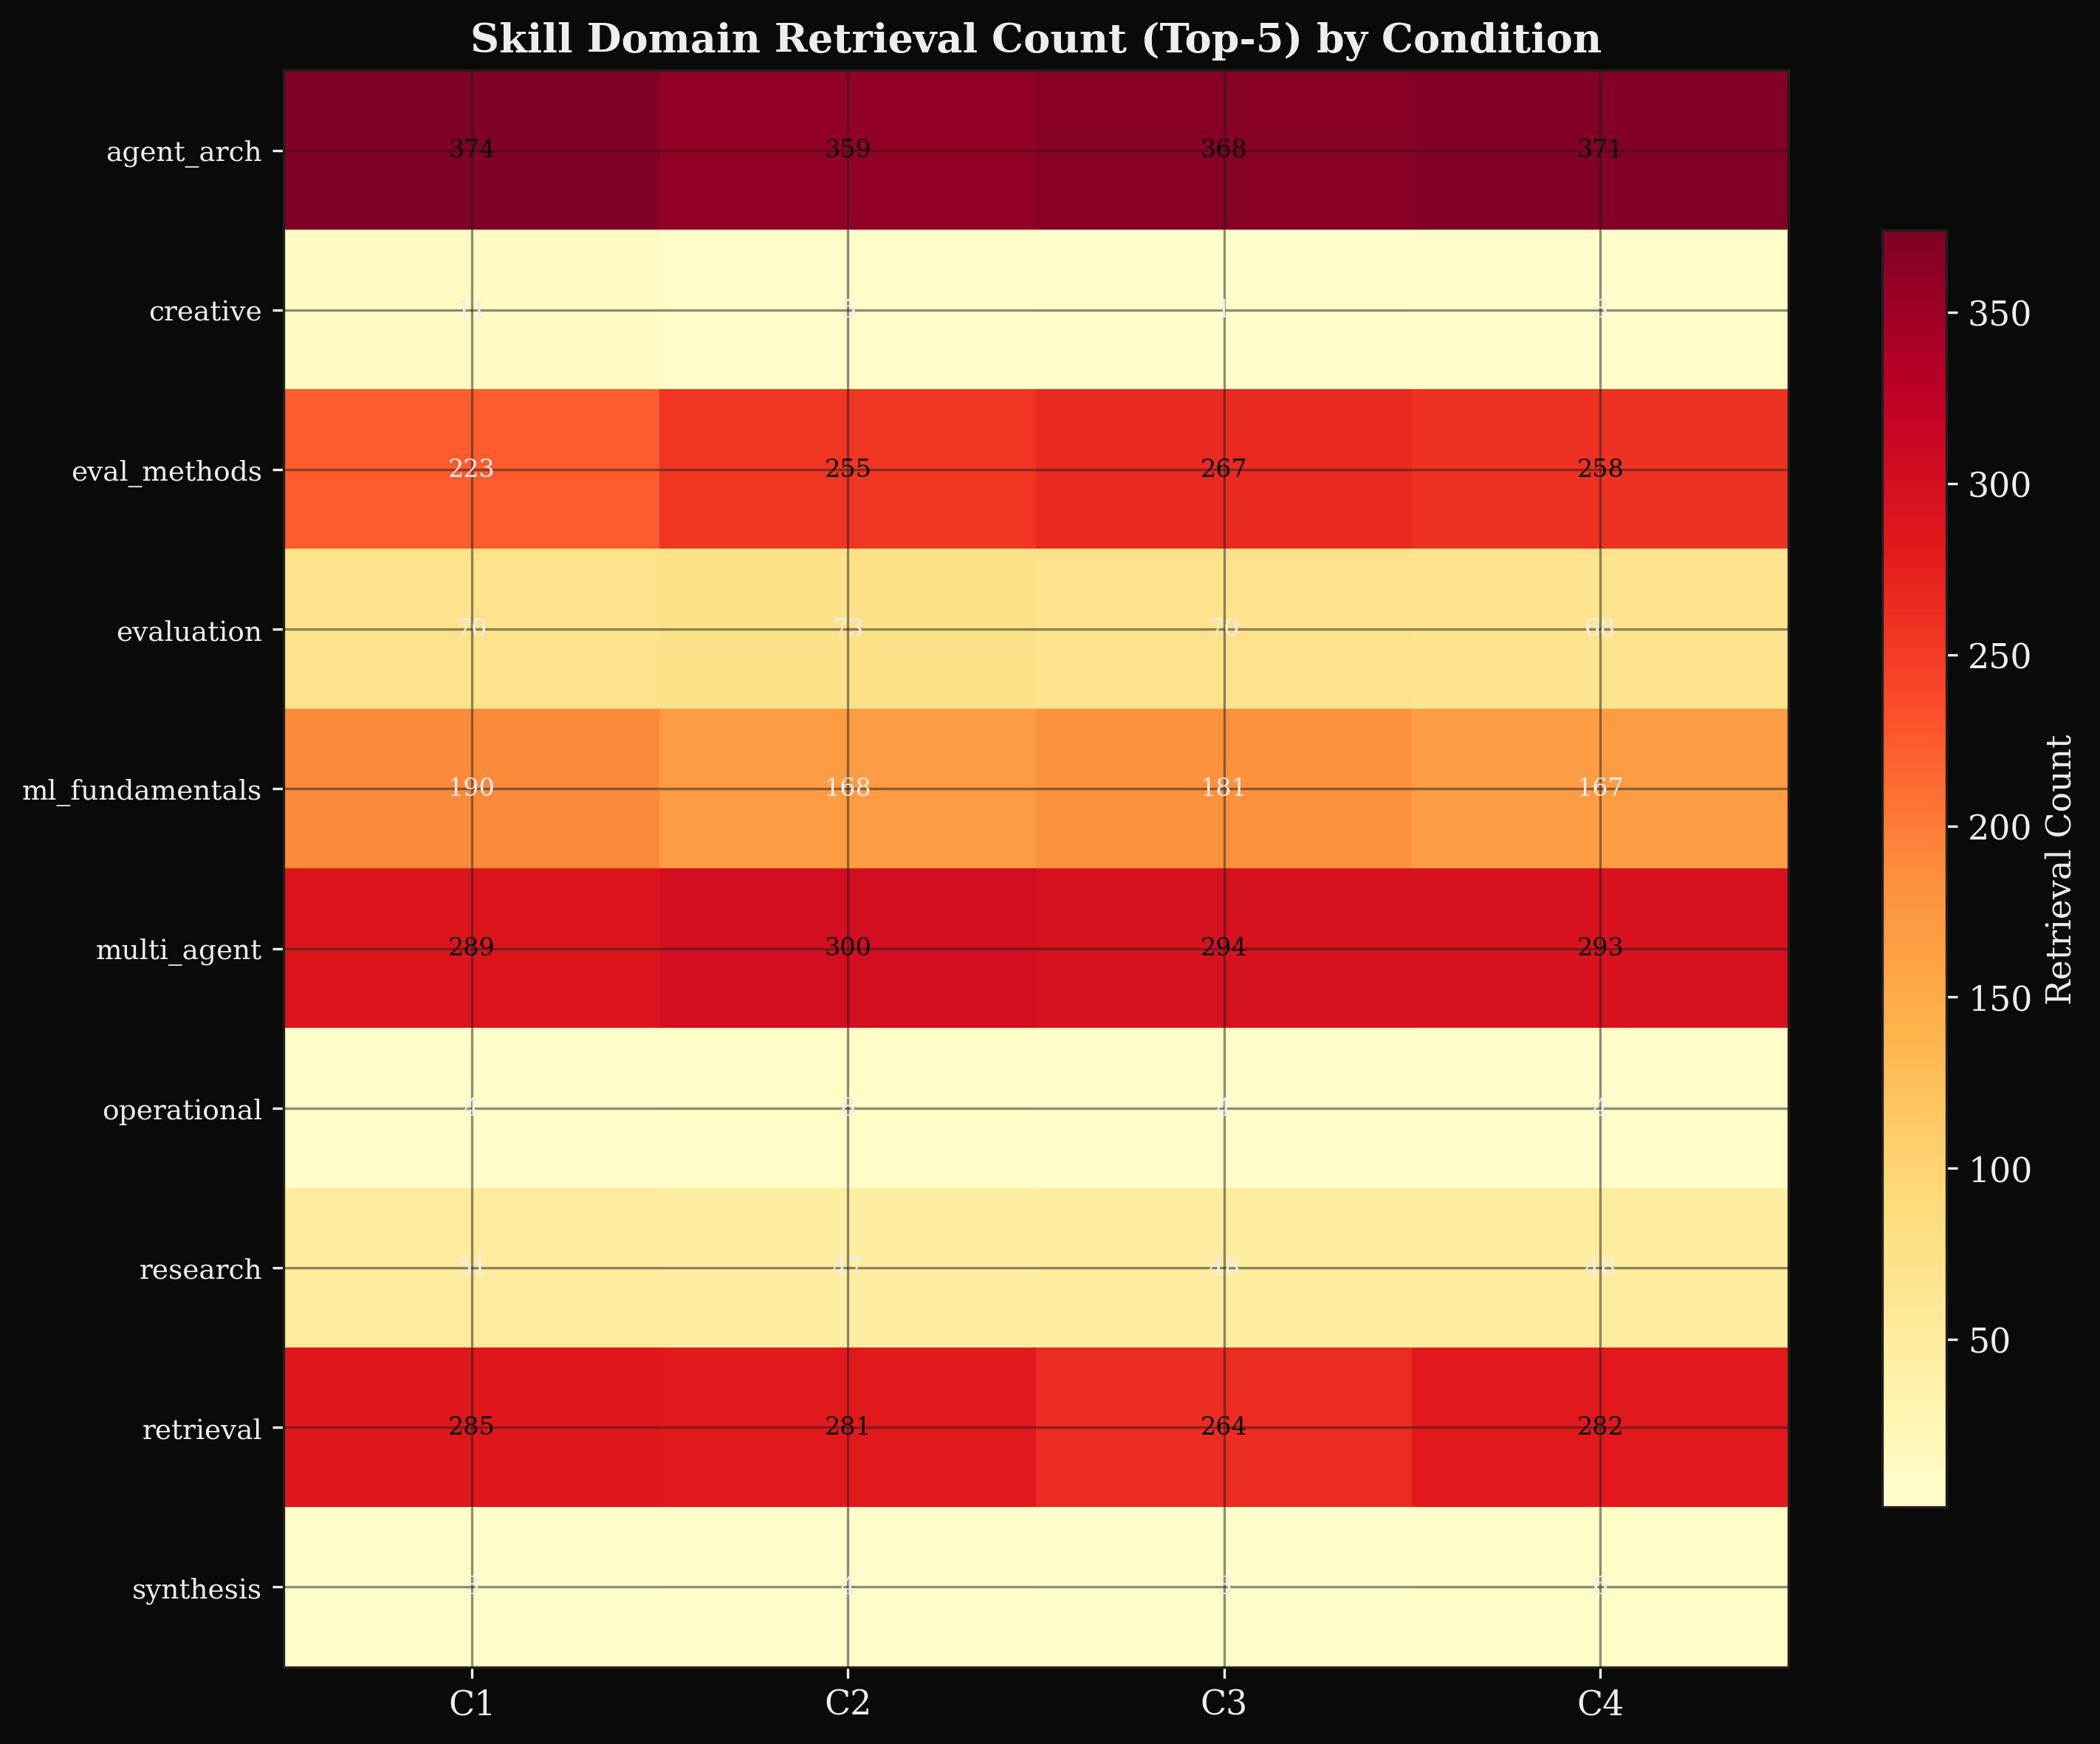
\includegraphics[width=\columnwidth]{../results/figures/figA9_domain_heatmap.png}
\caption{Mean token consumption by theme and condition (v3). Themes with the longest C1 outputs (retrieval\_systems, ml\_fundamentals) show the largest treatment effects, consistent with the output-driven mechanism: the rubric is most effective at reducing verbosity where verbosity is highest.}
\label{fig:v3_domain_heatmap}
\end{figure}

\paragraph{Two effects, now separable.}
Experiment~2 resolves the confound that limited Experiment~1's conclusions.
In v2, weight learning changed scores but not rankings (Jaccard $>$ 0.90), making it impossible to determine whether adaptive retrieval could contribute beyond the rubric prompt effect.
In v3, weight learning produces meaningfully different retrievals (mean Jaccard $<$ 0.60), with C3 achieving 26\% higher NDCG@5 than C1 and 20\% higher than C4.
Yet C4 achieves the largest token reduction ($-$19.7\% vs.\ C1), suggesting that \emph{the rubric prompt effect is the dominant mechanism for token reduction, while adaptive retrieval improves retrieval quality as measured by ground truth metrics}.

The two effects appear largely independent.
The rubric prompt effect reduces output token generation, a behavioral change in the LLM that does not depend on which skills were retrieved.
The adaptive retrieval effect improves the quality of retrieved skills, a change in the retrieval system that does not directly reduce token consumption when the rubric already constrains output verbosity.
This decomposition explains why C4 achieves the best efficiency (lowest mean tokens at 4{,}429, lowest output tokens at 2{,}537) while C3 achieves the best retrieval quality (highest NDCG@5 at 0.469, highest MRR at 0.411).

% Outlier Robustness Analysis — for inclusion in Section 5
% v3 re-run data (n=1200, 300 per condition, max_tokens=16384)

\subsection{Robustness to Outliers}
\label{sec:outlier_robustness}

With truncation cascades eliminated (\texttt{max\_tokens}$=$16{,}384), all four conditions produce relatively well-behaved distributions.
Mean-to-median ratios range from 1.08 (C4) to 1.15 (C2), with no extreme runaway episodes.
The single multi-step episode (C1, task~023, 21{,}259 tokens) is a moderate outlier at $6.4\sigma$ from the C1 mean.

To verify that the efficiency gains are not driven by a few high-token episodes, we apply progressively aggressive outlier filters, removing episodes exceeding $\mu + k\sigma$ for each condition independently at $k \in \{1, 2, 3\}$ (Table~\ref{tab:outlier_robustness}).

\begin{table}[t]
\centering
\small
\begin{tabular}{lccccc}
\toprule
\textbf{Filter} & \textbf{C1 mean} & \textbf{C2 mean} & \textbf{C3 mean} & \textbf{C4 mean} & \textbf{Best $\Delta$C1} \\
\midrule
None       & 5{,}517 & 4{,}824 & 4{,}830 & 4{,}429 & $-$19.7\% \\
$+3\sigma$ & 5{,}355 & 4{,}698 & 4{,}699 & 4{,}309 & $-$19.5\% \\
$+2\sigma$ & 5{,}190 & 4{,}533 & 4{,}555 & 4{,}224 & $-$18.6\% \\
$+1\sigma$ & 4{,}732 & 4{,}193 & 4{,}181 & 3{,}998 & $-$15.5\% \\
\bottomrule
\end{tabular}
\caption{Outlier robustness analysis. Each row removes episodes exceeding $\mu + k\sigma$ \emph{within each condition independently}. The treatment effect is stable across cutoffs (15--20\% reduction), confirming that the output-driven efficiency gain is distributed across the full episode population rather than driven by a few extreme episodes. ``Best $\Delta$C1'' reports the largest reduction among C2--C4 at each cutoff.}
\label{tab:outlier_robustness}
\end{table}

Two observations emerge.
First, the treatment effect is robust: even at the most aggressive filter ($+1\sigma$, which removes 39--48 episodes per condition), C4 still reduces mean tokens by 15.5\% relative to C1.
The stability across cutoffs (19.7\% raw $\rightarrow$ 15.5\% at $+1\sigma$) confirms that the effect is distributed across the full population of episodes, not concentrated in a few prevented catastrophes.
Second, unlike Experiment~1 where C1's mean was dominated by a catastrophic tail (mean/median ratio of 2.1$\times$), Experiment~2's clean distributions (all ratios $<$1.15) indicate that the output-driven mechanism operates consistently across all episodes.


\subsection{The Rubric Prompt Effect}
\label{sec:confound}

Experiment~1 revealed that C4 achieves the best token efficiency despite weak bandit convergence, suggesting a dominant prompt engineering effect.
Experiment~2 confirms and clarifies this finding in a more controlled setting: with truncation cascades eliminated, the rubric effect manifests as output compression rather than multi-step prevention.
C4 reduces mean tokens by 19.7\% while showing only weak bandit convergence (max posterior mean${=}$0.472), modest retrieval quality improvement (NDCG@5${=}$0.374 vs.\ C3's 0.469), and the lowest output token count (2{,}537 per episode).

The rubric prompt effect functions as a metacognitive anchor: by requiring the LLM to evaluate retrieval quality, regardless of whether that evaluation is used for adaptation, the rubric structures the response in a way that reduces verbose, exploratory output.
This has a methodological implication: \emph{any future work on adaptive retrieval in RAG systems must include a rubric-only control condition to isolate retrieval adaptation effects from prompt structuring effects.}

The contribution of weight learning is real but largely independent: C3 achieves substantially better retrieval (NDCG@5${=}$0.469 vs.\ C4's 0.374, $+$25\%) without improving token efficiency over C4.
This suggests that retrieval quality and token efficiency are partially independent outcomes in this setting, with the rubric's output-constraining effect introducing a ceiling: once the rubric has compressed output length, further retrieval quality improvements have limited room to produce additional token savings.
Improving retrieval quality through weight learning is valuable in its own right, ensuring the LLM receives the most relevant context, but the efficiency gains from the rubric's output-constraining effect are available without any learning at all.


\section{Discussion}
\label{sec:discussion}
% Section 6: Discussion (~0.75 pages)

\subsection{Disentangling Prompt Effects from Retrieval Effects}

Experiment~2 reveals that multi-step prevention, the apparent mechanism in Experiment~1, was a truncation artifact: only 1 of 1{,}200 episodes triggered multi-step reasoning.
The actual mechanism is \emph{output-driven efficiency}: the feedback rubric constrains LLM generation length directly (C4 output tokens 33\% below C1), acting as a metacognitive anchor that reduces verbose exploration rather than preventing reasoning spirals.

This has an immediate practical implication: any retrieval-augmented system can reduce token consumption by appending a structured feedback rubric, even without adaptive retrieval, a result independent of our Thompson Sampling contribution (see Appendix Figures~\ref{fig:token_trend} and~\ref{fig:theme_heatmap}).
The effect scales with task complexity (12\% for easy, 21\% for medium and hard) and operates consistently across all themes.

Experiment~2 also reveals a \emph{second} mechanism that was invisible in the small-library setting: retrieval differentiation.
With Jaccard overlap dropping from ${>}$0.90 to 0.52--0.59 (Table~\ref{tab:v3_results}), weight presets now produce genuinely different skill sets, and C3's retrieval quality gains (NDCG@5 $+$26.3\%, MRR $+$35.9\% vs.\ C1) break through the saturation ceiling diagnosed in Experiment~1.
The limitation was not fundamental to the R/I/V decomposition, but rather a consequence of insufficient library diversity.

\subsection{Input Assessment vs.\ Output Assessment}

Our design deliberately avoids output-level self-assessment~\citep{pan2024feedback}.
The empirical evidence (no detectable rating drift over 579 iterations in a prior deployment, 1{,}000 episodes in Experiment~1, and 1{,}200 episodes in Experiment~2) supports this choice.
Rating distributions in the first 50 episodes are statistically indistinguishable from the final 50 episodes across all dimensions ($p > 0.3$, Kolmogorov--Smirnov test; see Appendix Figure~\ref{fig:rating_stability}).
Beyond stability, the ratings are \emph{informative}: composite Likert scores correlate positively with ground-truth NDCG@5 ($r{=}0.33$, $p{<}0.001$; $r{=}0.44$ for C2 and C3), confirming that higher ratings correspond to genuinely better retrieval.
\citet{khalaf2025itrh} recently extended the ICRH finding to inference-time reward hacking, where best-of-$n$ sampling and inference-time alignment degrade quality; our input-assessment design is robust to both variants.

The principle is transferable: any system using LLM self-assessment in a feedback loop should evaluate upstream signals (inputs, context, retrieval) rather than downstream outputs to avoid self-referential reward inflation.

\subsection{When Does Weight Learning Matter?}

\begin{table}[t]
\centering
\small
\begin{tabular}{lrr}
\toprule
\textbf{Design / Metric} & \textbf{Exp.~1 (v2)} & \textbf{Exp.~2 (v3)} \\
\midrule
Skills              & 50 generic      & 205 domain-specific \\
Weight presets      & 5               & 12 \\
Tasks $\times$ conds & 250 $\times$ 4 & 300 $\times$ 4 \\
\texttt{max\_tokens} & 4{,}096        & 16{,}384 \\
\midrule
C1 mean tokens      & 6{,}481        & 5{,}517 \\
Multi-step rate (C1) & 11.6\%         & 0.3\% \\
\midrule
Jaccard C1--C2      & 0.904           & 0.585 \\
Jaccard C1--C3      & 0.909           & 0.517 \\
Jaccard C1--C4      & 0.848           & 0.573 \\
C3 NDCG@5           & ---             & 0.469 \\
C3 MRR              & ---             & 0.411 \\
\midrule
C2/C3 convergence   & importance      & pure\_relevance \\
C4 convergence      & none            & weak (importance) \\
Primary mechanism   & multi-step prev.\ & output compression \\
\bottomrule
\end{tabular}
\caption{Design changes and outcomes across experiments. Experiment~2's expanded library and de-saturated dimensions enable weight learning to produce differentiated retrieval (Jaccard $<$ 0.60), while eliminating truncation cascades reveals output compression as the primary efficiency mechanism.}
\label{tab:v2v3_comparison}
\end{table}

Experiment~1 shows that weight learning is inert with small, generic skill libraries where dimensions are saturated (Table~\ref{tab:v2v3_comparison}).
The mechanism is straightforward: Thompson Sampling's posterior width reflects uncertainty about each arm's quality, but when all presets retrieve nearly identical skill sets (Jaccard $> 0.90$), the observed reward variance is dominated by noise rather than genuine preset differences.
The posterior converges, but to a distinction without a difference.

Experiment~2 establishes the boundary condition.
With 205 domain-specific skills and 12 weight presets, C3 converges to \texttt{pure\_relevance} ($E[\theta]{=}$0.749) within ${\sim}$50 tasks (changepoint at tasks 33--48), and its explanation embeddings appear to produce a higher-fidelity reward signal than C2's Likert ratings.
The threshold at which weight learning begins to matter requires two conditions to be met simultaneously: sufficient library diversity (enough domain-specific skills that weight changes produce different rankings) and sufficient dimension variance (de-saturating recency and importance so that the weight space is not effectively one-dimensional).
Experiment~1 failed the first condition; Experiment~2 satisfies both.

The C4 result in the expanded setting is informative: C4 \emph{does} converge (to \texttt{pure\_importance}, $E[\theta]{=}$0.472), but with a compressed recency dimension (mean${=}$0.136).
This represents a shift from Experiment~1, where C4 showed flat posteriors.
The feedback rubric focuses the LLM's output regardless of what the bandit does with the weights.
C4's token advantage is an output-driven efficiency effect: the rubric constrains the LLM's generation. C3's advantage is a retrieval engineering effect: the bandit learns to retrieve better skills, aided by higher-fidelity reward signals from explanation embeddings.
These two mechanisms appear largely independent and can be combined.

These observations yield a two-condition diagnostic for practitioners considering adaptive retrieval weights.
First, compute the pairwise Jaccard similarity of top-$k$ retrievals across a representative sample of weight configurations: if Jaccard $> 0.80$, weight learning cannot differentiate presets and the investment is wasted (see Appendix Figure~\ref{fig:jaccard_vs_tokens} for the relationship between overlap and token consumption).
Second, check dimension variance across the skill library: if any dimension has variance $< 0.10$ (as recency and importance did in v2 at ${\sim}0.95$), the scoring function collapses to relevance-only ranking regardless of weights.
The Experiment~1 to Experiment~2 transition demonstrates this diagnostic in action: addressing both conditions dropped mean Jaccard from $>$0.90 to 0.52--0.59 and produced the retrieval quality improvements reported in Section~\ref{sec:experiment_v3}.

In practice, start with the rubric-only baseline (C4), which captures output-driven efficiency without any bandit machinery.
Upgrade to adaptive weight learning only if the Jaccard diagnostic shows sufficient skill diversity and the dimension variance check confirms a meaningful weight space.
Thompson Sampling itself is cheap (12 Beta posteriors, episode-wise updates), but the surrounding instrumentation (parsing ratings, computing diagnostics, validating convergence) is not, and should be justified by expected retrieval quality gains.
Where both diagnostic conditions are met, the investment pays off quickly: C3 converges in ${\sim}$50 tasks, and the two mechanisms (output efficiency + retrieval adaptation) can be combined.

\subsection{Transferability Beyond RAG}

While our experiments operate within vector-based RAG, the two primary findings are not structurally dependent on the retrieval architecture:

\begin{enumerate}
\item \textbf{Metalevel input assessment} (evaluating retrieval inputs rather than task outputs to avoid reward hacking) applies to any system that uses LLM self-assessment in a feedback loop.
The absence of rating drift across 2{,}200+ episodes is a property of the reward design, not the retrieval architecture.

\item \textbf{Output-driven efficiency} (structured feedback rubrics reducing output tokens by 33\%) operates through prompt structure, not retrieval.
Any system that appends a structured evaluation rubric may observe similar output compression.
\end{enumerate}

The retrieval weight optimization itself is specific to the Park et al.\ (2023) paradigm and is most valuable for large-scale deployments (thousands of documents) where the corpus exceeds context-window limits and fine-tuning lacks sufficient training data.


\section{Conclusion}
\label{sec:conclusion}
% Section 7: Conclusion (~0.3 pages)

This work identifies two largely independent mechanisms in gradient-free retrieval weight learning for agent systems.
The first, \emph{output-driven efficiency}, operates through output length reduction: feedback conditions produce shorter, more focused outputs, reducing token consumption by up to 19.7\% (C4 vs.\ C1), consistent with more focused prompts from better-weighted retrieval.
The second, \emph{adaptive retrieval}, is a retrieval engineering effect: the bandit learns to retrieve qualitatively different and higher-quality skill sets, with C3 improving NDCG@5 by 26.3\% and MRR by 35.9\% over the fixed-weight control.
C3 converges strongly to \texttt{pure\_relevance} within approximately 50 tasks; C2 trends toward \texttt{pure\_relevance} but with a near-tie against \texttt{recency\_heavy}; C4 converges weakly to \texttt{pure\_importance}.
All treatment-vs-control differences are significant after Holm--Bonferroni correction.

The transition from Experiment~1 (50 generic skills) to Experiment~2 (205 domain-specific skills) reveals the boundary condition for weight learning.
With a small, saturated library, all weight configurations retrieve near-identical skill sets (Jaccard $>$ 0.90) and the bandit converges to a distinction without a difference.
Expanding the library and de-saturating embedding dimensions drops mean Jaccard to 0.52--0.59, a structural shift that enables weight differences to produce genuinely different retrievals.
Across 1,200 episodes (300 tasks $\times$ 4 conditions), the v3 results suggest that retrieval quality improvement and output-driven efficiency are largely separable effects that can compound when both mechanisms are active.

These findings yield a two-step practitioner diagnostic.
First, compute pairwise Jaccard similarity of top-$k$ retrievals across weight configurations: if Jaccard $>$ 0.80, weight learning cannot differentiate presets and the efficiency benefit alone may not justify the bandit machinery.
Second, check per-dimension variance across the skill library: if any dimension has variance $<$ 0.10, the scoring function collapses to effectively one-dimensional ranking regardless of weights.
Only when both checks pass does adaptive weight learning add value beyond a static weight baseline.

Our input-assessment reward design, evaluating retrieval inputs rather than task outputs, shows no detectable rating drift across 2{,}200+ episodes (1,000 in Experiment~1 and 1,200 in Experiment~2), supporting the strategy of avoiding self-referential reward loops identified by~\citet{pan2024feedback}.
Unlike gradient-based alternatives, the approach requires no labeled data and works with proprietary LLMs without fine-tuning access.

The most immediate extension is multi-model validation: testing whether the output-driven efficiency effect transfers beyond MiniMax M2.5 to frontier models with different verbosity profiles.
A second direction is adaptive skill libraries that grow or prune over time, introducing non-stationarity that the current bandit formulation does not handle.
A third direction is user-level diversity-aware metrics such as UDCG, which would capture whether adaptive weights improve not just relevance but topical coverage across retrieved skills.
A fourth direction is a comparative architecture study: evaluating Thompson Sampling adaptation within RAG against agentic keyword search and fine-tuning on the same task corpus, to determine where each approach dominates in the cost-performance landscape.
Finally, isolating the output-length reduction from content changes, via controlled ablations that hold response content fixed while varying prompt structure, would strengthen the causal claim behind the efficiency mechanism.


\section*{Limitations}
% Limitations section

\paragraph{Single model, synthetic tasks.}
All experiments use MiniMax M2.5 on a synthetic task corpus (300 tasks, five themes, three difficulty levels).
The output-driven efficiency mechanism may be sensitive to model-specific instruction-following behavior, and the 100\% task success rate means we measure token efficiency and retrieval quality but not response quality differences.
Validating these findings on frontier models and real user queries remains necessary.

\paragraph{Limited exploration budget.}
Thompson Sampling with 12 arms and 300 episodes per condition yields roughly 25 episodes per arm under uniform exploration.
C2 and C3 reach a stable selection pattern by approximately task 33--48 (changepoint analysis), with \texttt{pure\_relevance} dominating thereafter; however, the posterior continues to sharpen through episode 300.
C4's compressed posteriors (max $E[\theta]{=}0.472$) may reflect insufficient data rather than a fundamental property of anchor-based rewards; longer runs would clarify this.

\paragraph{No human quality evaluation.}
Our reward hacking assessment relies on rating stability (no detectable drift across 1{,}200 episodes) rather than independent quality judgment.
We cannot confirm that efficiency gains preserve output quality; the stability finding is consistent with reward hacking avoidance but does not prove it.
More broadly, token efficiency is a proxy metric: shorter outputs are not necessarily better outputs, and without human evaluation of response quality, the 12--20\% token reduction could reflect less thorough responses rather than more concise ones.

\paragraph{Confounded cross-experiment comparison.}
Experiments~1 and~2 differ in multiple design dimensions simultaneously (library size, skill specificity, number of presets, task difficulty distribution), so improvements cannot be attributed to a single factor.
The Jaccard overlap reduction from ${>}$0.90 to 0.52--0.59 confirms retrieval differentiation, but the overlap remains moderate.
Additionally, C4's anchor embedding parser compresses the recency dimension (mean 0.136 vs.\ importance 0.62 and relevance 0.55), effectively reducing feedback to two dimensions and limiting the bandit's ability to distinguish recency-weighted presets.

\paragraph{Static skill library and parser specificity.}
Skills were fixed throughout each experiment; a production system with evolving skills would face non-stationarity that our bandit formulation does not address.
The feedback parser is also specific to MiniMax's output patterns (parse rates: 93--97\%), and the 5--7\% parse failure rate introduces noise into the reward signal.

\paragraph{Single experimental run.}
Results are from a single execution per condition with no repeated runs under different random seeds.
We cannot estimate seed-dependent variance or confirm reproducibility of the specific convergence patterns (e.g., C3's lock-in to \texttt{pure\_relevance} by task 44).
The fixed-seed task shuffling ensures deterministic condition assignment but does not address the inherent stochasticity of LLM generation and Thompson Sampling exploration.

\paragraph{Single-annotator ground truth.}
Ground truth skill annotations (1--3 relevant skills per task) were created by a single annotator.
Inter-annotator agreement was not assessed, and the subjective nature of skill relevance means that retrieval quality metrics (NDCG@5, MRR, hit rate) reflect one person's judgments rather than a consensus standard.

\paragraph{Missing ablation controls.}
The experimental design lacks a rubric-only ablation (appending the feedback rubric without any bandit updates) and a comparison against standard MAB baselines (e.g., UCB1, $\epsilon$-greedy).
Without a rubric-only control that explicitly disables the bandit, the rubric prompt effect and adaptive retrieval effect cannot be fully disentangled.
Additionally, C3's explanation embedding storage constitutes a potential confound: C3 maintains additional semantic information not available to C2, so its superior retrieval quality may partly reflect richer stored context rather than better reward signals alone.

\paragraph{Dimension label semantics.}
The ``importance'' dimension is computed as a Laplace-smoothed historical success rate, which more closely tracks usage frequency than intrinsic importance.
This labeling may affect how the LLM interprets the feedback rubric, potentially conflating frequency-based and quality-based assessments in its dimension ratings.

\paragraph{Narrow evaluation domain.}
All tasks and skills are drawn from a single domain (AI/ML research), limiting generalizability to other knowledge domains where the relative informativeness of recency, importance, and relevance dimensions may differ substantially.

\paragraph{Narrow architectural evaluation.}
All experiments operate within the vector-based RAG paradigm.
Our 205-skill library is small enough that agentic keyword search, long-context models, or fine-tuning could plausibly match or exceed our retrieval quality without the bandit machinery.
We do not evaluate whether the Thompson Sampling mechanism or the self-assessment reward signal transfers to these alternative architectures, though the mechanisms are not structurally dependent on vector retrieval (see Section~\ref{sec:discussion}).

\paragraph{Related work scope.}
The related work section does not discuss connections to learning-to-rank (LTR) methods, which optimize ranking functions via supervised or semi-supervised learning, or to the metacognitive monitoring literature in cognitive science, which provides a theoretical grounding for the input-assessment concept.
These connections represent directions for future positioning.


\section*{Reproducibility Statement}
All code, data, and configuration files required to reproduce both experiments are publicly available at \url{https://github.com/kusp-dev/retrieval-weight-experiment} (code under Apache 2.0; data under CC BY 4.0).
The repository contains the synthetic task corpora (250 tasks for v2, 300 for v3), both skill libraries (50 and 205 skills), ground truth task--skill annotations, and all analysis scripts used to generate the figures and statistics reported in this paper.
Dependencies are specified in \texttt{pyproject.toml} (Python $\geq$3.11); a \texttt{Dockerfile} is provided for environment reproduction.
All hyperparameters, including RRF constant $k{=}60$, weight preset definitions, and Thompson Sampling $\text{Beta}(1,1)$ priors, are centralized in a single configuration file.
Task ordering is shuffled with a fixed seed (42) for deterministic condition assignment.
The test suite (238 unit and integration tests) validates retrieval, scoring, and bandit update logic.
Experiments were run on a Mac Mini M4 using the MiniMax M2.5 API for generation and Qwen3-Embedding-0.6B for local dense retrieval.
Total compute for both experiments was approximately 52 hours.


\section*{Ethics Statement}
\paragraph{Minimal ethical risk.}
This work poses minimal ethical risk.
All experiments use synthetic tasks designed by the authors; no human subjects were involved and no personally identifiable information was collected or processed.
The LLM's own assessments serve as the reward signal for bandit learning; no human annotators or crowd workers were employed.
The system generates only task-completion responses (e.g., summaries, analyses) with no capacity for harmful content production.

\paragraph{Compute and environmental impact.}
Total compute for both experiments was approximately 52 hours on a Mac Mini M4 (Apple Silicon, ${\sim}$20W TDP).
LLM inference used the MiniMax M2.5 commercial API; local embedding inference used Qwen3-Embedding-0.6B.
The energy footprint is modest: under 2~kWh for local computation across both experiments, negligible relative to model training runs.
API-side energy consumption is not disclosed by the provider but is bounded by the small scale of inference (${\sim}$2{,}200 episodes, ${\sim}$4{,}000 tokens per episode).

\paragraph{Broader impact.}
The primary societal implication of this work is efficiency: reducing token consumption in LLM systems lowers inference costs and energy use at deployment time.
The input-assessment reward design, by avoiding output-level self-assessment, may contribute to safer feedback loops in deployed agentic systems by reducing the risk of reward hacking.
However, the techniques---input-assessment reward and gradient-free parameter learning---could in principle be applied to optimize configuration parameters in systems that serve harmful content; we recommend that practitioners apply these methods only within systems that maintain appropriate content safety guardrails.
We release all code and data under open licenses (Apache 2.0 for code, CC BY 4.0 for data) to support reproducibility and downstream research.


\bibliographystyle{tmlr}
\bibliography{references}

\appendix
% Appendix

\section{Rubric Text}
\label{app:rubric}

\subsection{Conditions 2 and 3 (Likert Scale)}

The following text is appended to the agent's prompt when skills are retrieved and injected:

\begin{quote}
\small\ttfamily\raggedright\noindent
RETRIEVAL FEEDBACK --- MANDATORY (if skills were provided above):\\{}
[RETRIEVAL EFFECTIVENESS]\\{}
You were provided with skills retrieved using three scoring dimensions:\\{}
- RECENCY: How recent/fresh the skill is\\{}
- IMPORTANCE: How important it was previously flagged\\{}
- RELEVANCE: How well it semantically matches your current task\\[\medskipamount]
Rate how useful EACH dimension was for helping you complete this specific task.\\{}
You MUST use exactly this format (one rating per line, number only):\\[\medskipamount]
Recency: <single number 1-5, where 1=irrelevant to task, 5=essential>\\{}
Importance: <single number 1-5>\\{}
Relevance: <single number 1-5>\\[\medskipamount]
Brief explanation (2-3 sentences):\\{}
- Which dimension was most valuable and why?\\{}
- Which dimension was least valuable and why?\\{}
- What KIND of skills would have been even more helpful?\\{}
[/RETRIEVAL EFFECTIVENESS]
\end{quote}

\subsection{Condition 4 (Qualitative, Separated Questions)}

\begin{quote}
\small\ttfamily\raggedright\noindent
RETRIEVAL FEEDBACK --- MANDATORY (if skills were provided above):\\{}
[RETRIEVAL EFFECTIVENESS]\\{}
Evaluate how useful each retrieval dimension was for this specific task.\\{}
You MUST respond inside each tagged section below with 2-3 sentences.\\[\medskipamount]
[RECENCY EVALUATION]\\{}
How important was the freshness/timing of the retrieved skills for this task?\\{}
Were recently-used skills more helpful than older ones, or did timing not matter?\\{}
[/RECENCY EVALUATION]\\[\medskipamount]
[IMPORTANCE EVALUATION]\\{}
How important was the proven track record of the retrieved skills for this task?\\{}
Did you need battle-tested, reliable skills, or would untested ones have worked?\\{}
[/IMPORTANCE EVALUATION]\\[\medskipamount]
[RELEVANCE EVALUATION]\\{}
How important was the subject matter match of the retrieved skills for this task?\\{}
Were topically aligned skills essential, or could off-topic skills have helped?\\{}
[/RELEVANCE EVALUATION]\\{}
[/RETRIEVAL EFFECTIVENESS]
\end{quote}

\section{Anchor Embedding Design}
\label{app:anchors}

Table~\ref{tab:anchors} summarizes the calibration results for the separated-question anchor parser (Condition~4).
Anchors describe qualitatively different scenarios rather than degree variations to maximize embedding distance.

The anchor texts for each dimension are:

\paragraph{Recency anchors.}
\textbf{Low:} ``I already knew the current state of the art for this task. The retrieved skills, whether old or new, were redundant---freshness made no difference because the fundamentals haven't changed.''
\textbf{Mid:} ``I used a standard approach that has been around for a while. Recently used skills gave me useful context for incremental improvements, but I could have solved it with older knowledge alone.''
\textbf{High:} ``This task required cutting-edge techniques that have only emerged recently. Only the most recently practiced skills had methods I wasn't already familiar with. Older skills were obsolete.''

\paragraph{Importance anchors.}
\textbf{Low:} ``I solved this task from first principles and experimentation. Whether the skills had been successfully applied before didn't affect my approach---I would have tried any method regardless of track record.''
\textbf{Mid:} ``Proven skills gave me more confidence in my approach, but I would have still explored unproven alternatives if needed. Track record was a useful signal but not decisive.''
\textbf{High:} ``This task was too high-stakes to experiment with unproven methods. I relied exclusively on skills with demonstrated success because failure would have been costly. Untested approaches were unacceptable.''

\paragraph{Relevance anchors.}
\textbf{Low:} ``I needed creative cross-domain thinking for this task. Skills from unrelated fields sparked novel ideas just as much as on-topic skills. Semantic match to the task description was irrelevant.''
\textbf{Mid:} ``I needed a mix of deep domain knowledge and lateral thinking. On-topic skills provided essential structure, but insights from adjacent fields also contributed meaningfully to my solution.''
\textbf{High:} ``This task demanded deep, specialized domain expertise. Only skills directly about the exact topic were useful---off-topic skills were noise that distracted from the precise technical requirements.''

\begin{table}[t]
\centering
\small
\begin{tabular}{lccccc}
\toprule
\textbf{Dim.} & \textbf{Low} & \textbf{Mid} & \textbf{High} & \textbf{Spread} & \textbf{Order} \\
\midrule
Recency & 0.175 & 0.409 & 0.745 & 0.570 & \checkmark \\
Importance & 0.207 & 0.542 & 0.924 & 0.717 & \checkmark \\
Relevance & 0.162 & 0.344 & 0.822 & 0.660 & \checkmark \\
\bottomrule
\end{tabular}
\caption{Anchor calibration results ($\tau=0.05$, 9 synthetic texts per dimension). Spread $=$ high $-$ low. Order preserved (low $<$ mid $<$ high) across all 27 test texts.}
\label{tab:anchors}
\end{table}

\section{Skill Library Design}
\label{app:skills}

\paragraph{Experiment 1 (v2).}
50 meta-skills across 5 domains: research (10), creative (10), synthesis (10), evaluation (10), operational (10).
Skills are procedural and domain-general (e.g., ``Systematic Literature Review,'' ``Hypothesis Generation Framework'').

\paragraph{Experiment 2 (v3).}
205 domain-specific skills: 30 base skills plus 175 specialized skills distributed across 5 themes (${\sim}$35 per theme: ML Fundamentals, Agent Architectures, Multi-Agent Systems, Evaluation Methods, Retrieval Systems).
Specialized skills are designed to be relevant to specific task types within each theme, ensuring that weight configurations can produce different top-5 retrievals.

\section{Task Corpus Construction}
\label{app:tasks}

\paragraph{Experiment 1 (v2).}
250 tasks: 100 easy, 100 medium, 50 hard.
Tasks are distributed across 5 themes (50 per theme).
Difficulty is determined by expected reasoning depth: easy tasks require single-step retrieval, medium tasks require integration of 2--3 skills, hard tasks require multi-step reasoning or cross-domain synthesis.

\paragraph{Experiment 2 (v3).}
300 tasks: 50 easy, 100 medium, 150 hard.
The shift toward harder tasks increases the expected impact of retrieval quality on performance.
Ground truth skill annotations (1--3 relevant skills per task) enable measurement of retrieval precision via ground truth hit rate.

\section{Thompson Sampling vs.\ UCB}
\label{app:ts_vs_ucb}

We chose Thompson Sampling (TS) over Upper Confidence Bound (UCB) variants for four reasons specific to our problem setting.

\paragraph{Stochastic rewards from noisy self-assessment.}
LLM dimension ratings are inherently noisy: the same retrieval configuration applied to similar tasks produces reward variance of 0.15--0.25 across episodes.
TS models this naturally via Beta posteriors: uncertainty is represented probabilistically, and exploration is driven by posterior width rather than a manually tuned confidence bound.
UCB1 computes $\bar{x}_k + c\sqrt{\ln t / n_k}$, requiring selection of the exploration constant $c$.
In our setting, reward noise is non-uniform across arms (presets that emphasize relevance have lower variance than balanced presets), making a single $c$ suboptimal.
TS adapts to per-arm variance without tuning.

\paragraph{Exploration without hyperparameters.}
$\epsilon$-greedy and UCB both require exploration parameters ($\epsilon$, $c$) that affect convergence speed and final regret.
TS draws directly from the posterior: wide posteriors produce high-variance samples (exploration), and narrow posteriors produce concentrated samples (exploitation).
This property is especially valuable when the number of episodes per condition is fixed by experimental budget (250--300), so there is no opportunity to tune exploration parameters via a validation split.

\paragraph{Finite-arm optimality.}
With $K \in \{5, 12\}$ discrete weight presets, TS achieves the Lai--Robbins lower bound on asymptotic regret for Bernoulli rewards~\citep{agrawal2012analysis}; with our continuous pseudo-count updates, the bound is approximate but convergence behavior is preserved in practice.
We deliberately keep the action space discrete (presets on the weight simplex) rather than attempting continuous optimization, because: (a) the reward signal is too noisy for gradient estimation, (b) the simplex constraint complicates continuous bandit methods, and (c) 5--12 presets provide sufficient coverage of qualitatively different retrieval strategies.

\paragraph{Compatibility with non-stationarity.}
While our experimental design is stationary (tasks are shuffled), a production deployment would face concept drift as the skill library evolves.
TS with discounted posteriors (multiplying $\alpha_k, \beta_k$ by a decay factor each episode) handles non-stationarity gracefully, whereas UCB confidence bounds must be explicitly re-calibrated.
We do not use discounting in the controlled experiment, but the architecture supports it.

\paragraph{Empirical validation.}
We verified the choice empirically using data from both experiments (1{,}000 v2 episodes and 1{,}200 v3 episodes).
Cumulative regret was computed against an oracle that always selects the highest-reward arm.
Across conditions C2--C4, TS regret is sublinear and stabilizes by episode 100--150 (see Figure~\ref{fig:convergence_curves} for posterior trajectories and Figure~\ref{fig:cumulative_regret} for cumulative regret), consistent with the theoretical $O(\sqrt{KT \ln T})$ bound.
In v3, C3 converges to \texttt{pure\_relevance} with posterior mean 0.749 by approximately episode 44, demonstrating rapid lock-in when the reward signal is informative.

\section{Statistical Methods}
\label{app:stats}

All primary comparisons use bootstrap confidence intervals (10,000 resamples) rather than parametric tests, due to extreme variance heterogeneity across conditions (C1 SD$=$24{,}746 vs.\ C4 SD$=$2{,}037 in v2; C1 SD$=$2{,}449 vs.\ C4 SD$=$1{,}429 in v3).
We report two-sided bootstrap $p$-values computed as the fraction of resamples where the difference crosses zero.
For v3, we additionally report Kruskal--Wallis omnibus tests (non-parametric), Mann--Whitney $U$ for pairwise comparisons with Holm--Bonferroni correction (six comparisons), and Cohen's $d$ effect sizes.
Effect sizes are reported as percentage reduction in mean token consumption relative to C1.

\section{Supplementary Figures}
\label{app:figures}

\begin{figure}[t]
\centering
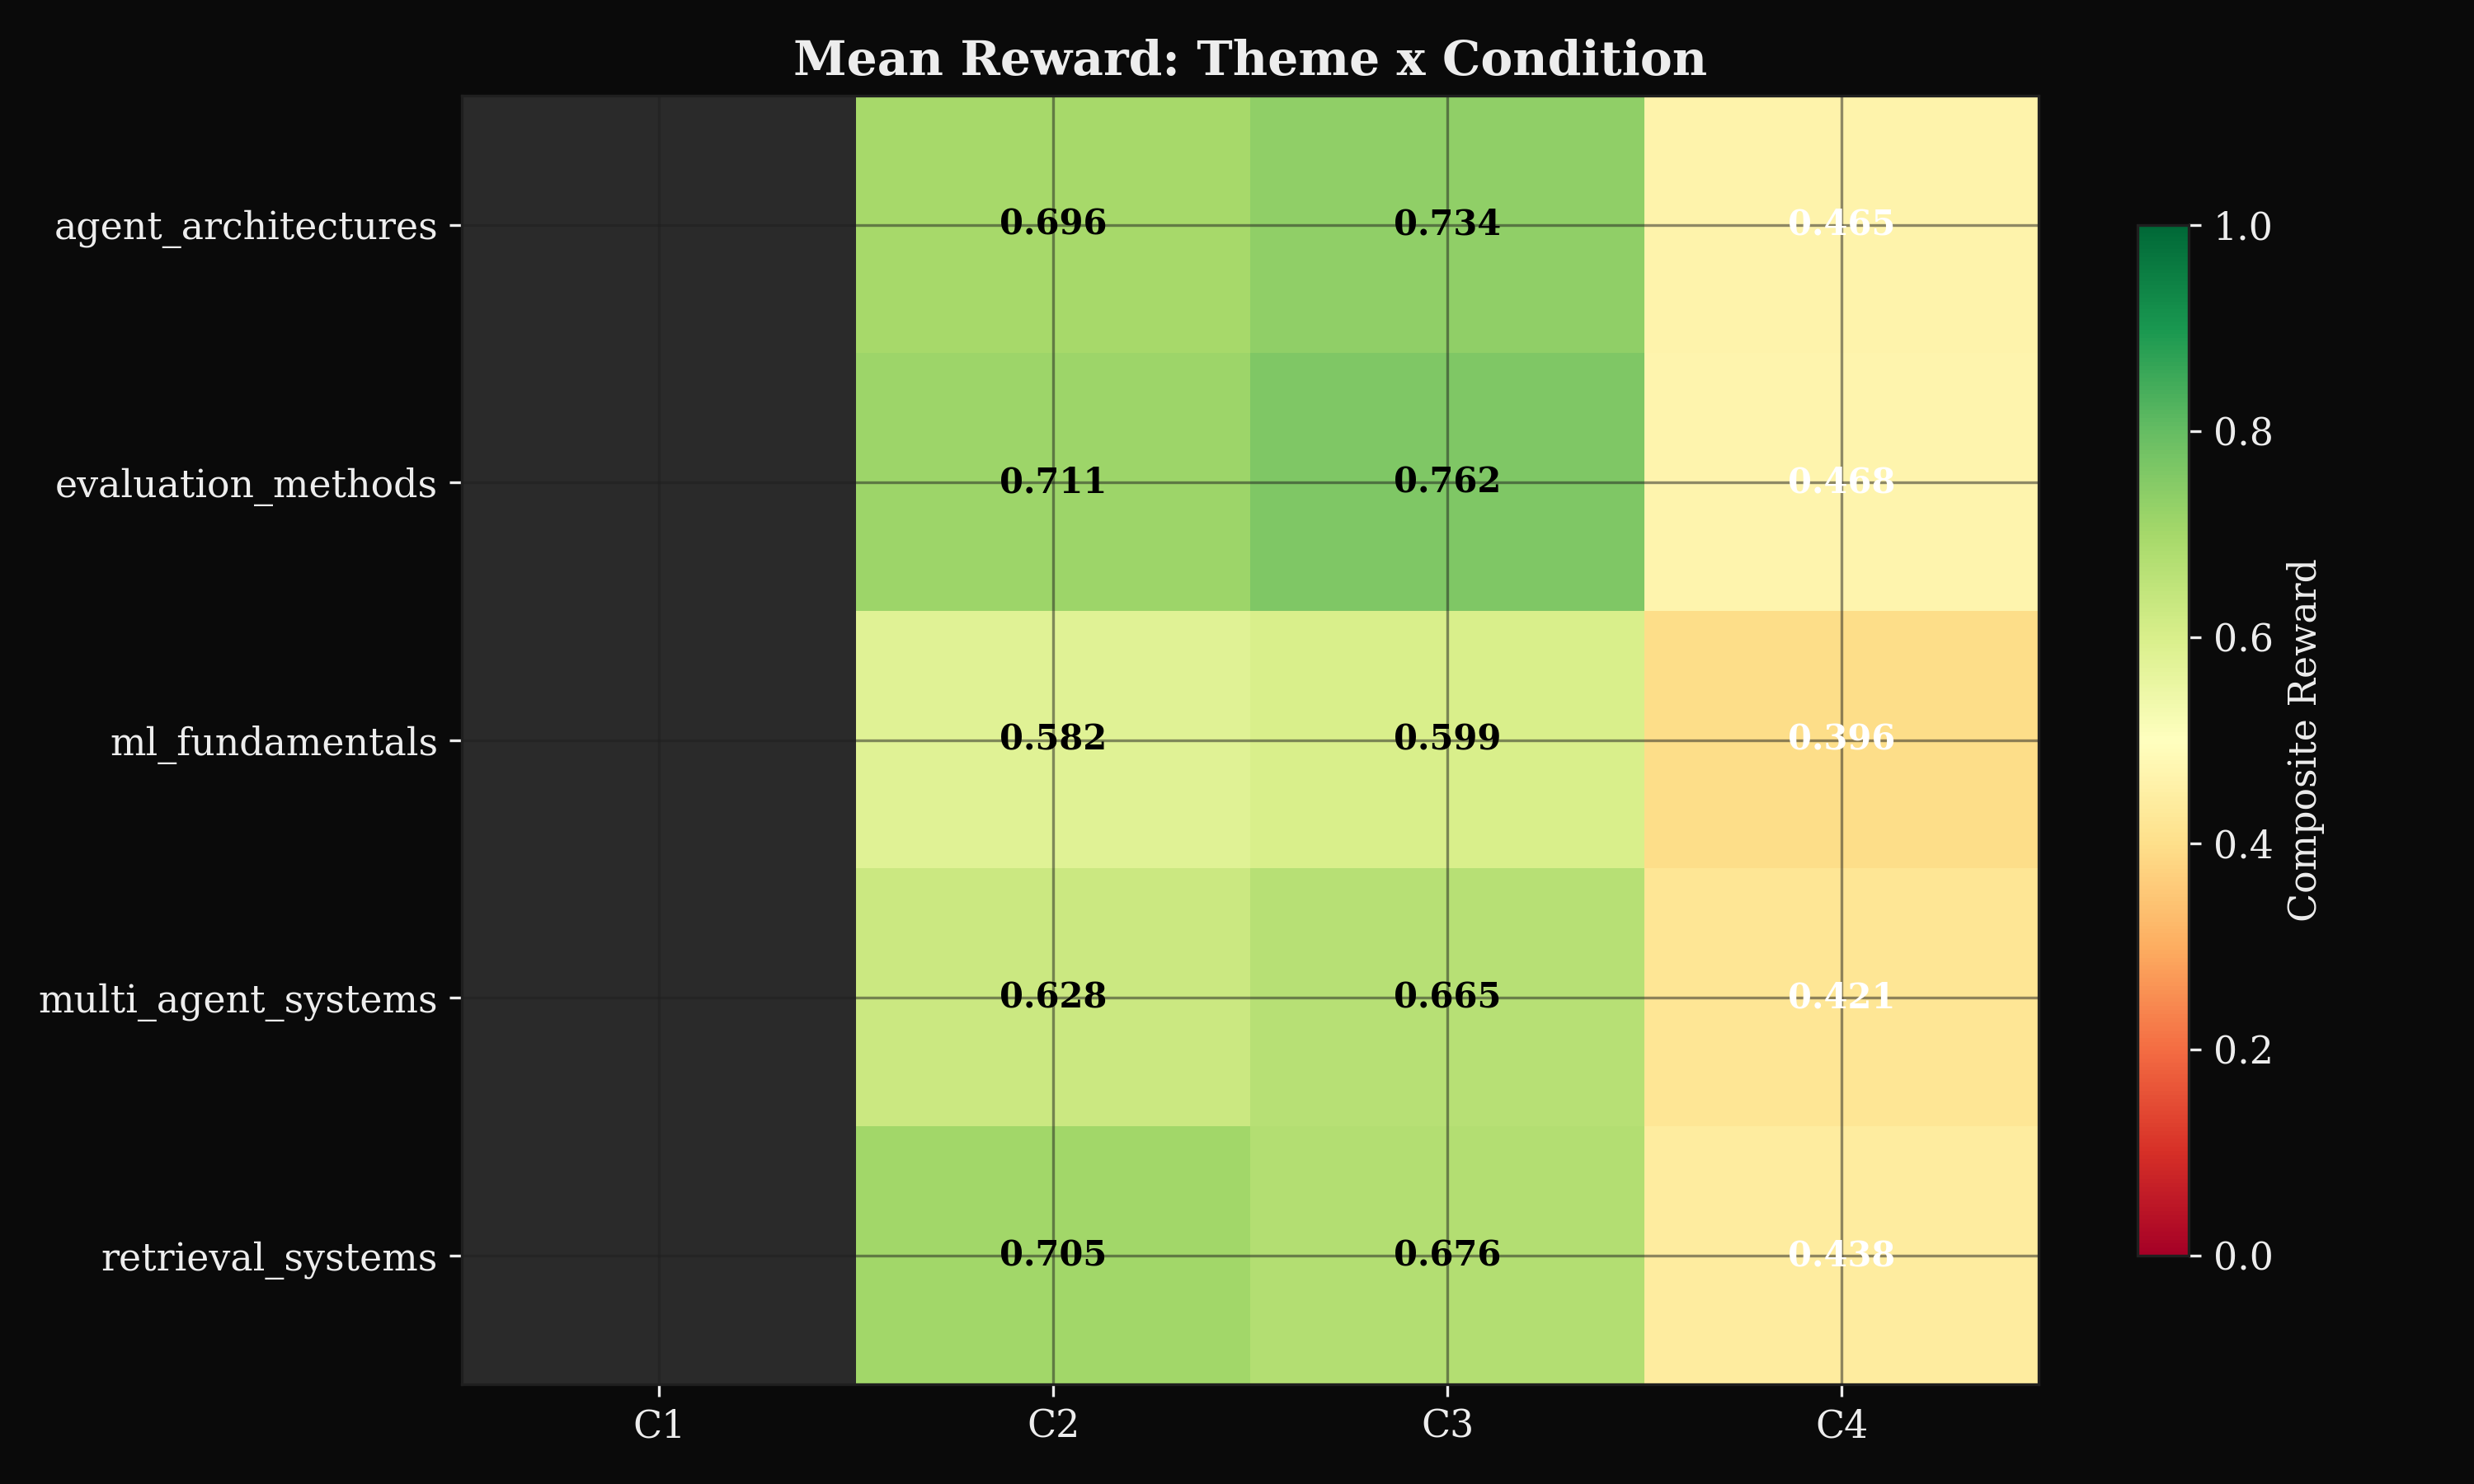
\includegraphics[width=\columnwidth]{../results/figures/fig3_theme_heatmap.png}
\caption{Mean reward by condition and theme. Reward variation across themes is modest ($<$0.15 range), consistent with the rubric prompt effect dominating over theme-specific retrieval differences.}
\label{fig:theme_heatmap}
\end{figure}

\begin{figure}[t]
\centering
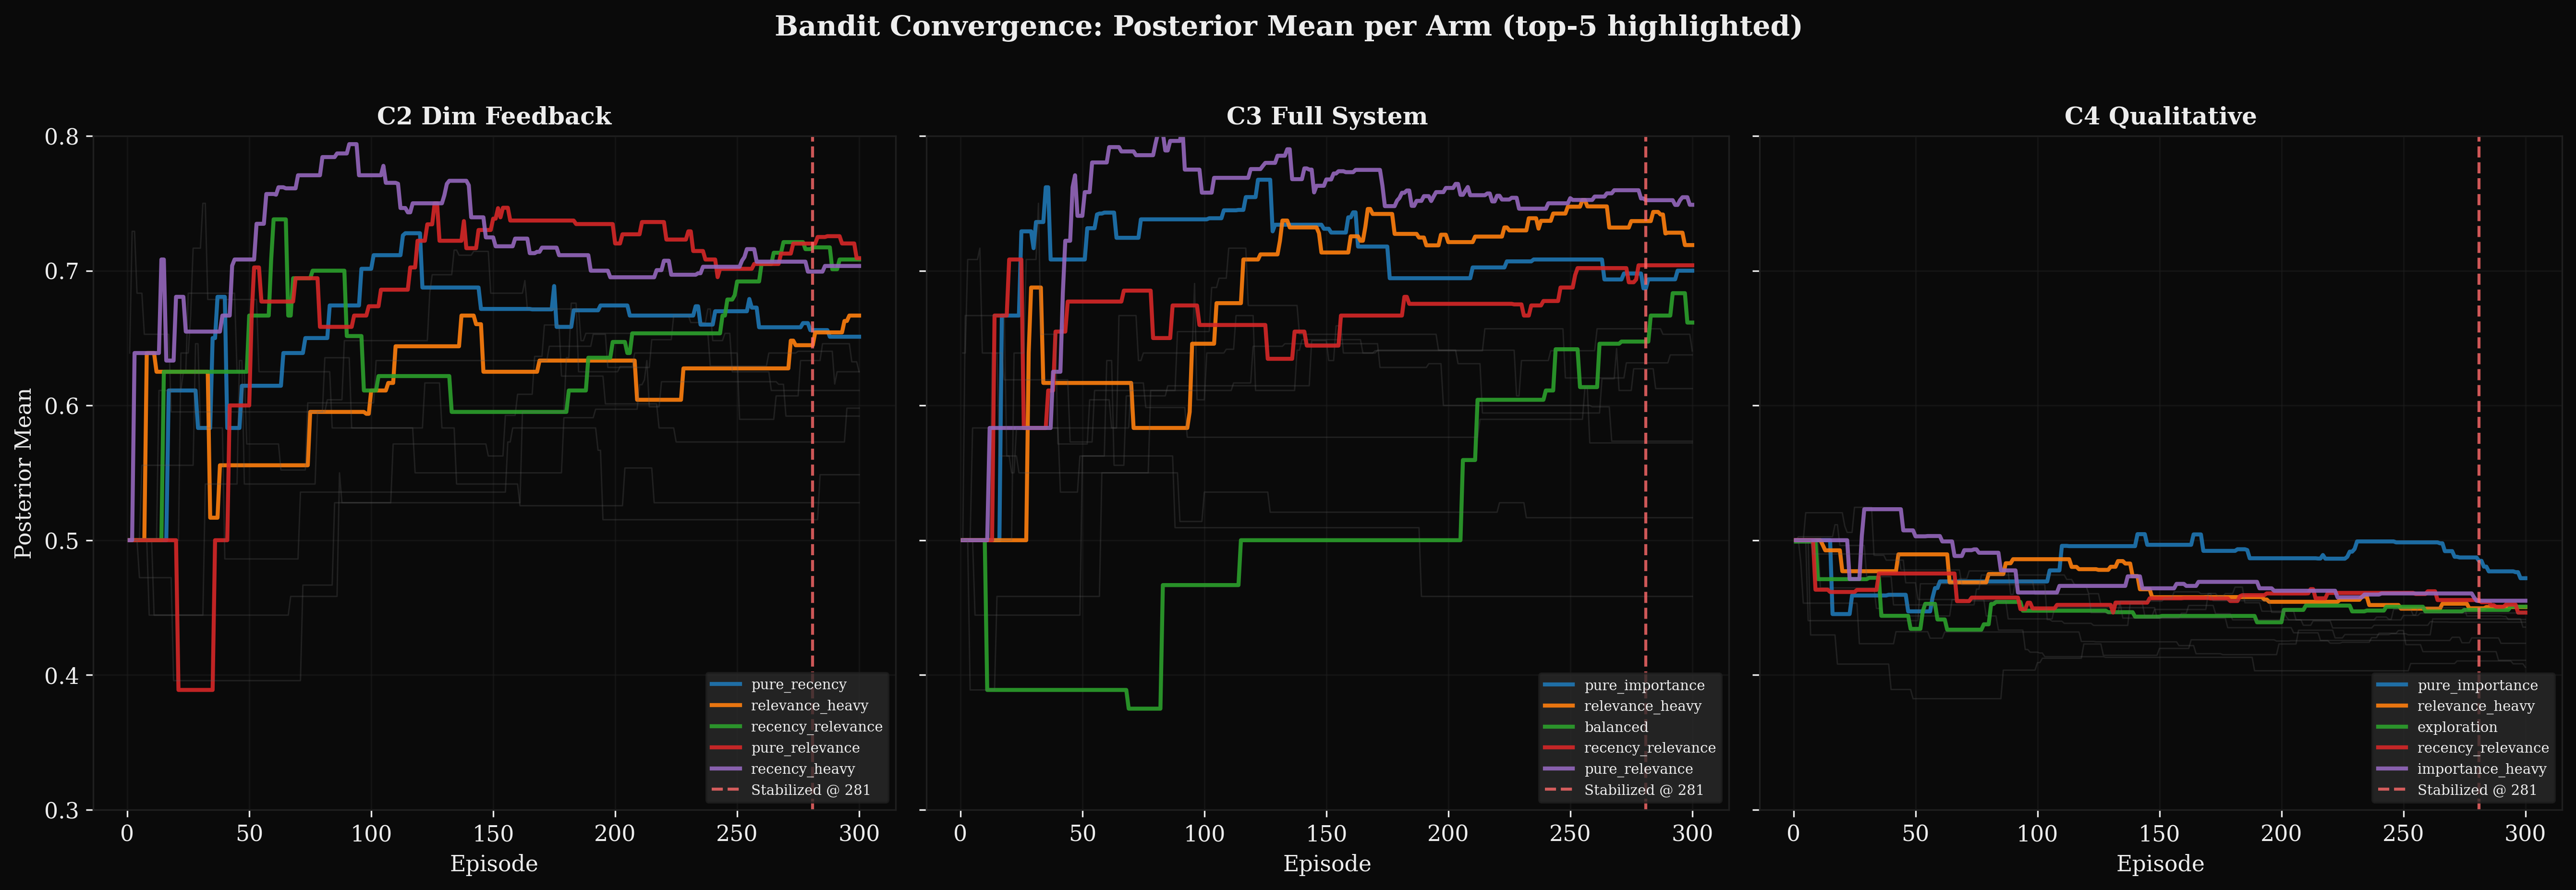
\includegraphics[width=\columnwidth]{../results/figures/fig2_convergence_curves.png}
\caption{Thompson Sampling posterior mean trajectories over episodes (v3, 12 arms, top 5 highlighted). C2 and C3 both converge toward \texttt{pure\_relevance}; C3 reaches a stable selection pattern by task 33--48. C4 shows compressed posteriors with all arms near 0.45, reflecting the anchor parser's limited discriminative signal.}
\label{fig:convergence_curves}
\end{figure}

\begin{figure}[t]
\centering
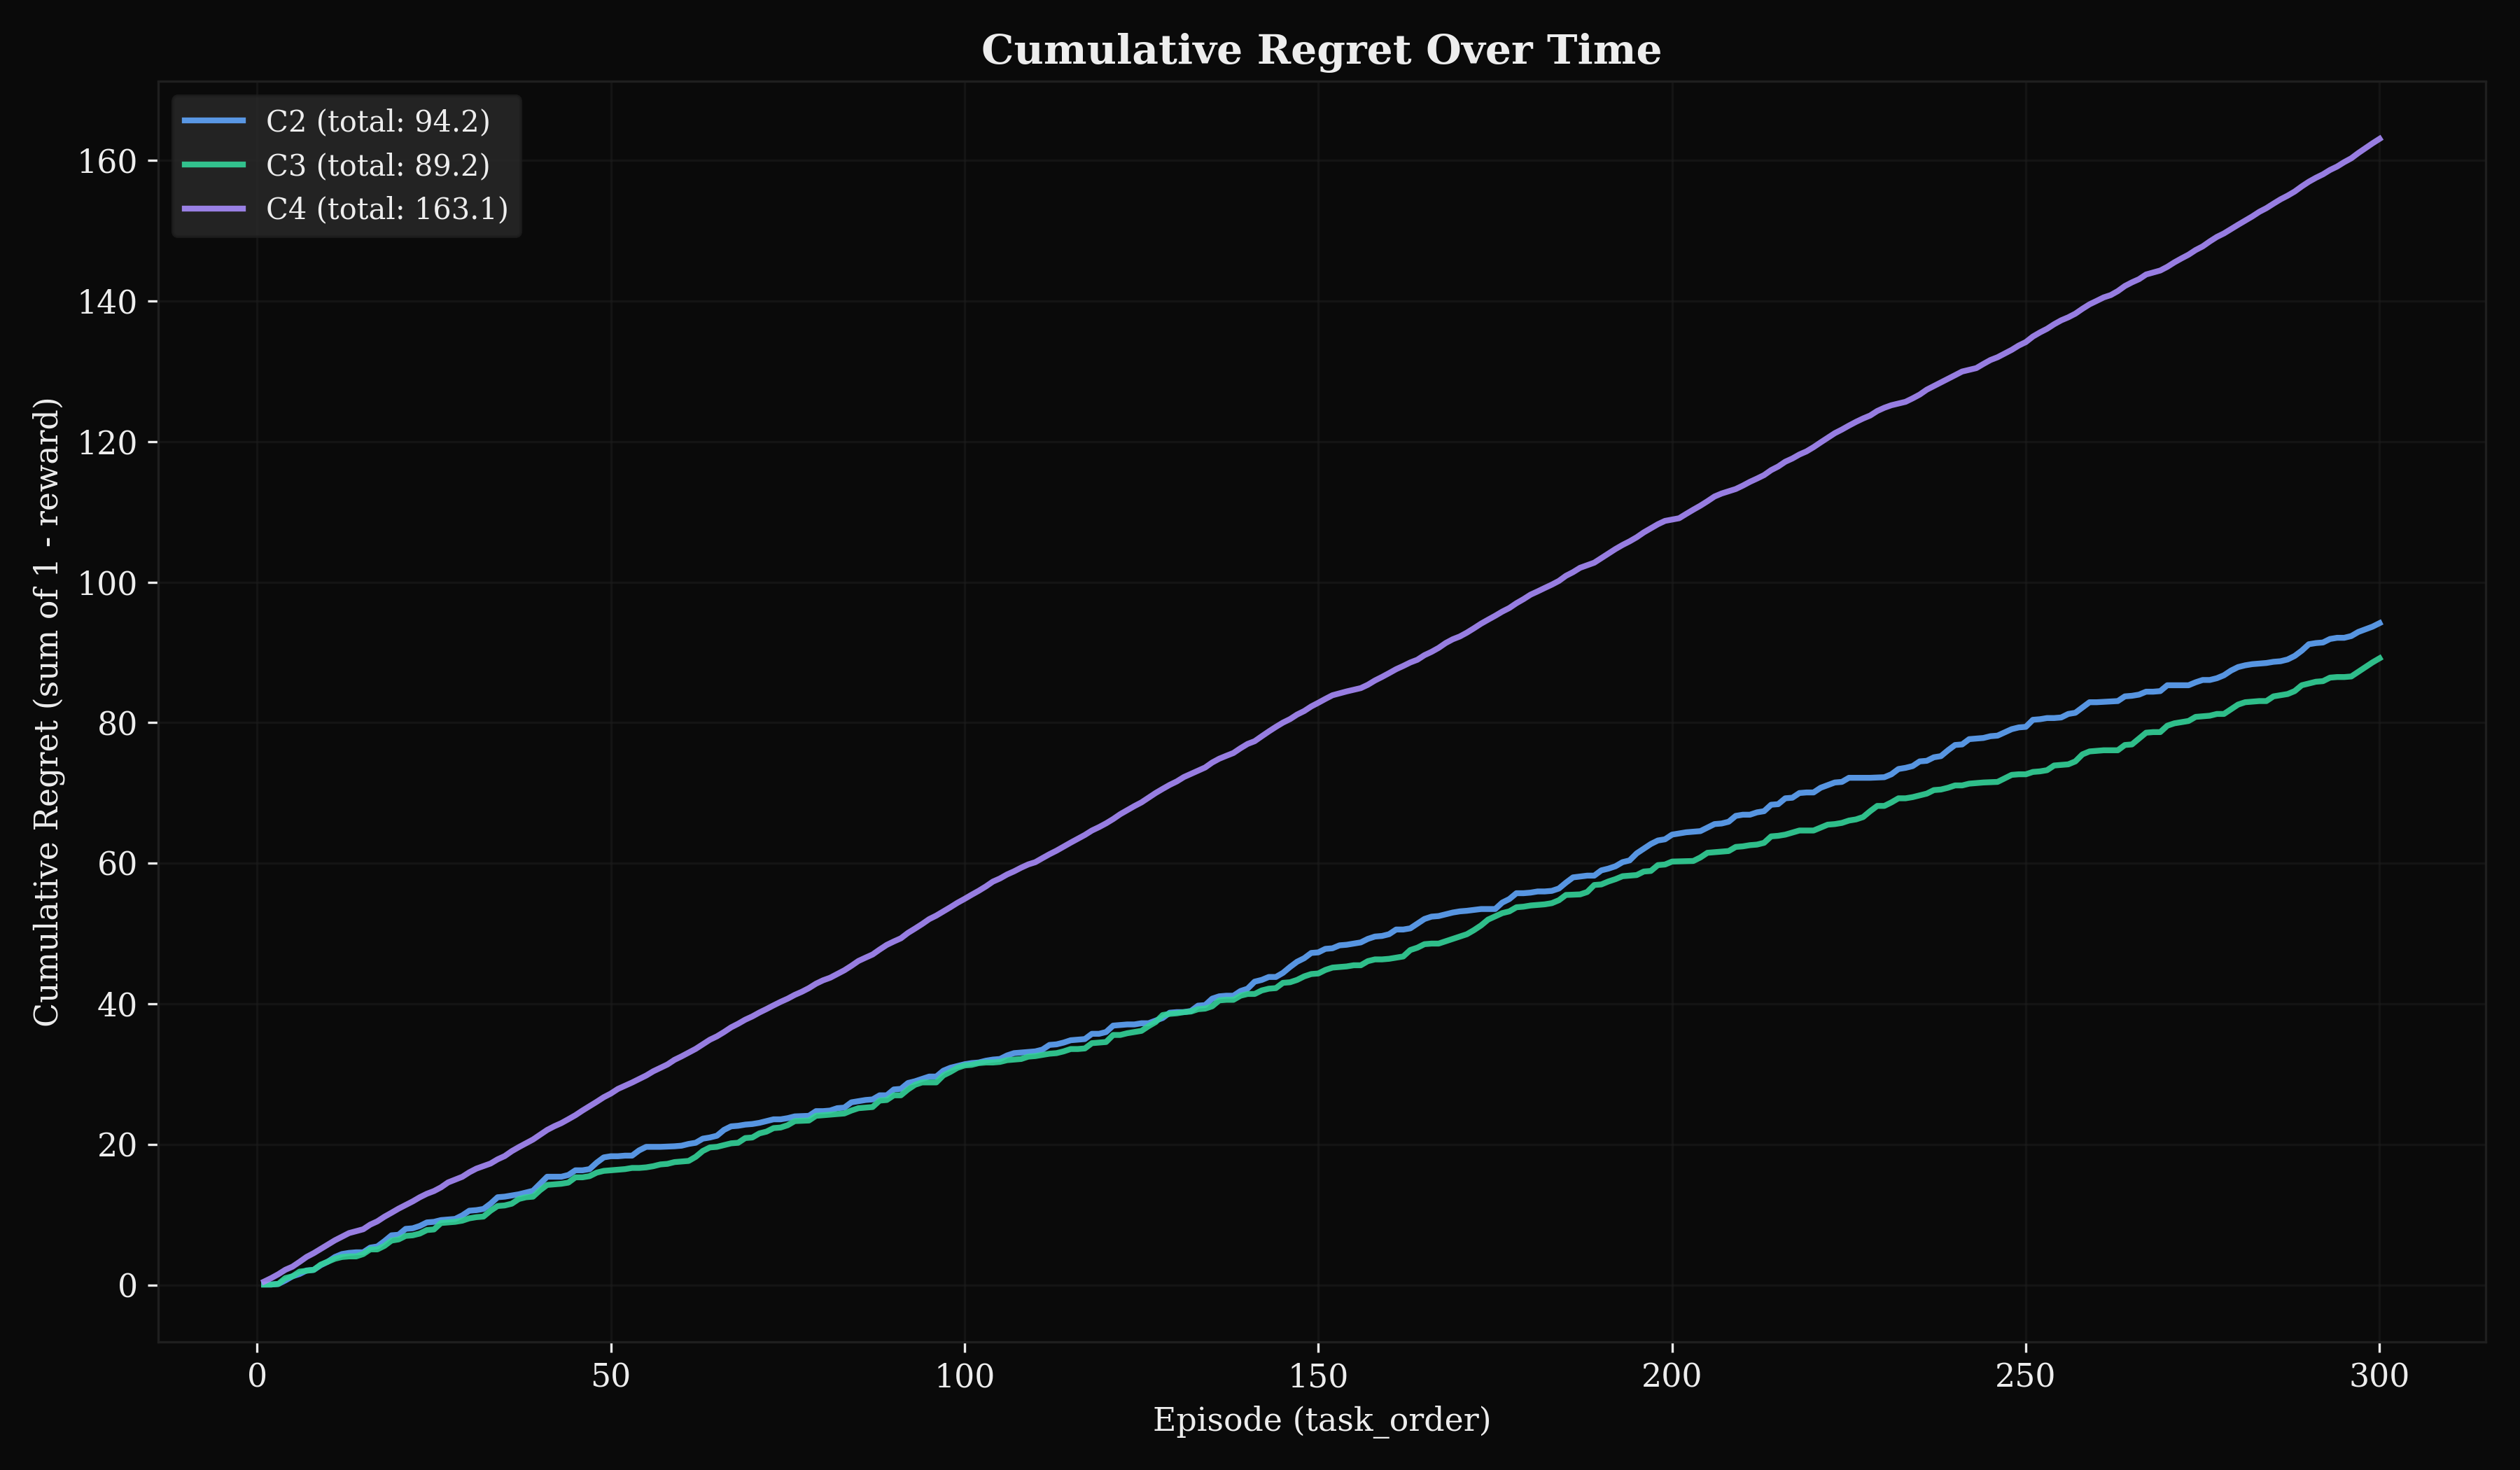
\includegraphics[width=\columnwidth]{../results/figures/fig5_cumulative_regret.png}
\caption{Cumulative regret for Thompson Sampling in C2, C3, and C4. Regret is computed against an oracle that always selects the highest-reward arm. C2 and C3 show sublinear regret growth consistent with convergence; C4's linear regret reflects compressed reward variance preventing arm differentiation.}
\label{fig:cumulative_regret}
\end{figure}

% fig7_jaccard_trajectory.png is now included in experiment_v3.tex (Figure~\ref{fig:v3_jaccard_trajectory})
% with a caption covering both v2 and v3 data. Removed duplicate here.

\begin{figure}[t]
\centering
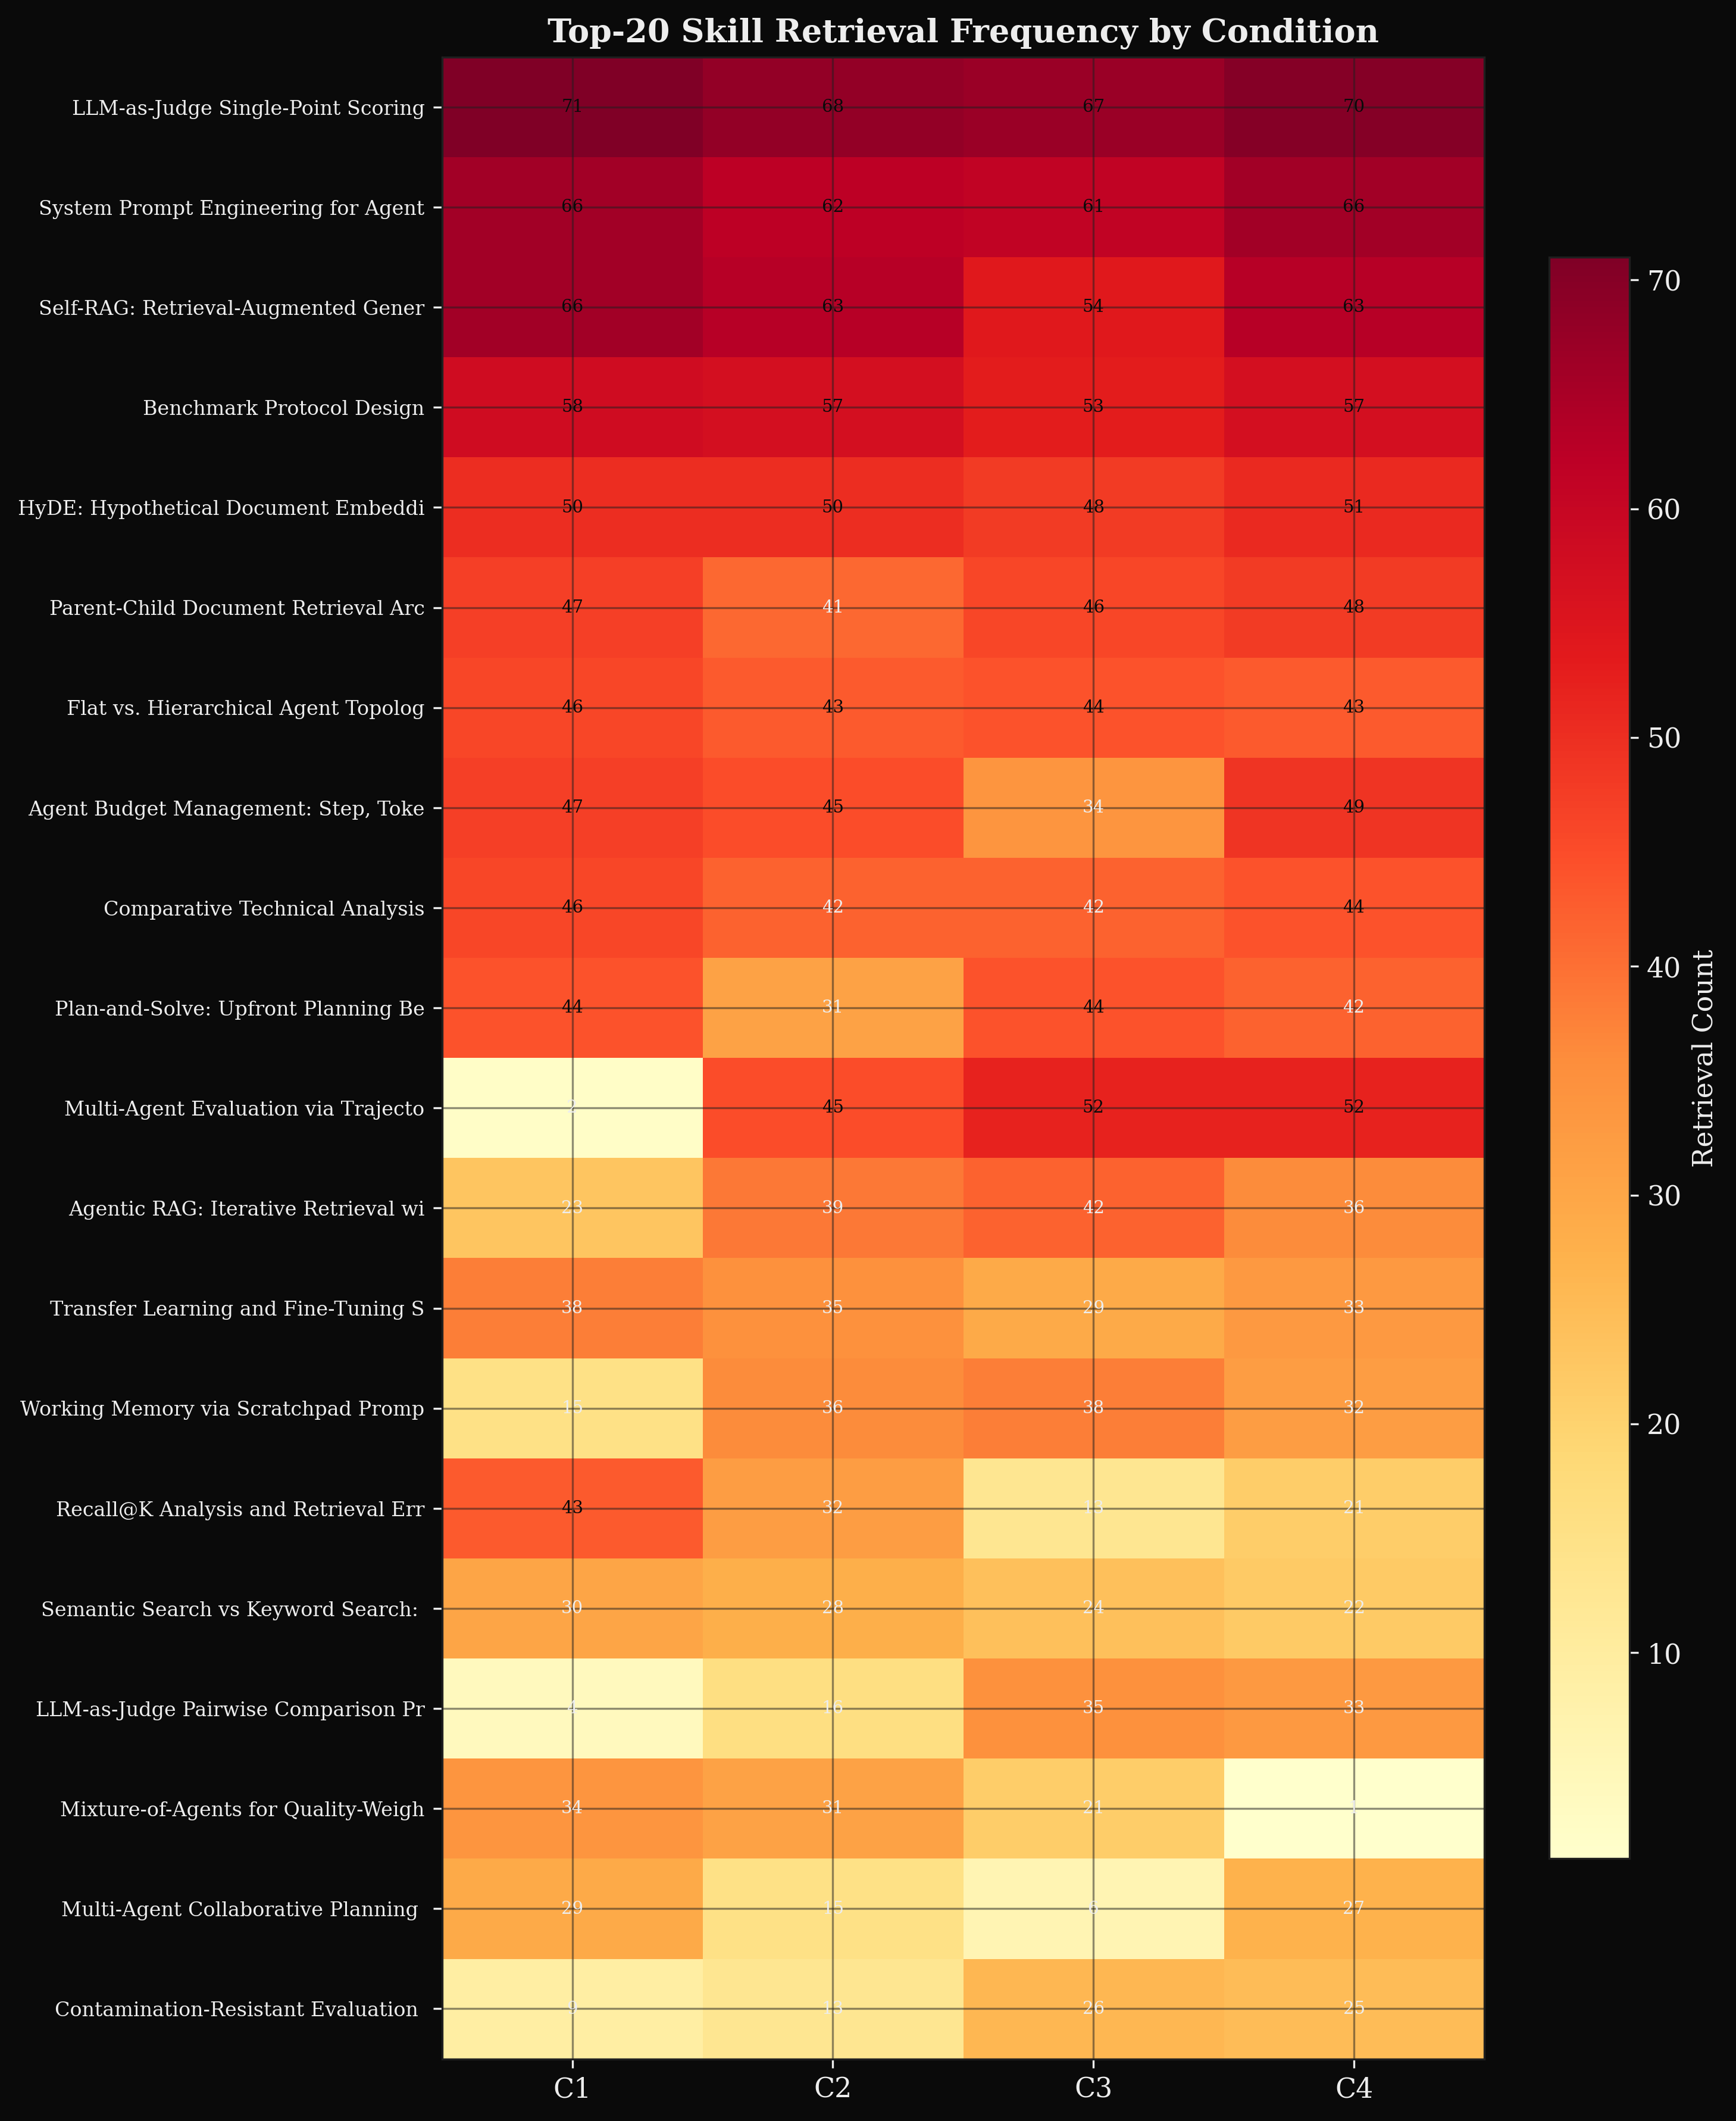
\includegraphics[width=\columnwidth]{../results/figures/figA1_skill_retrieval_heatmap.png}
\caption{Skill retrieval frequency heatmap. A small number of generic skills dominate retrieval across all conditions, explaining why weight changes do not change the top-5 set.}
\label{fig:skill_heatmap}
\end{figure}

\begin{figure}[t]
\centering
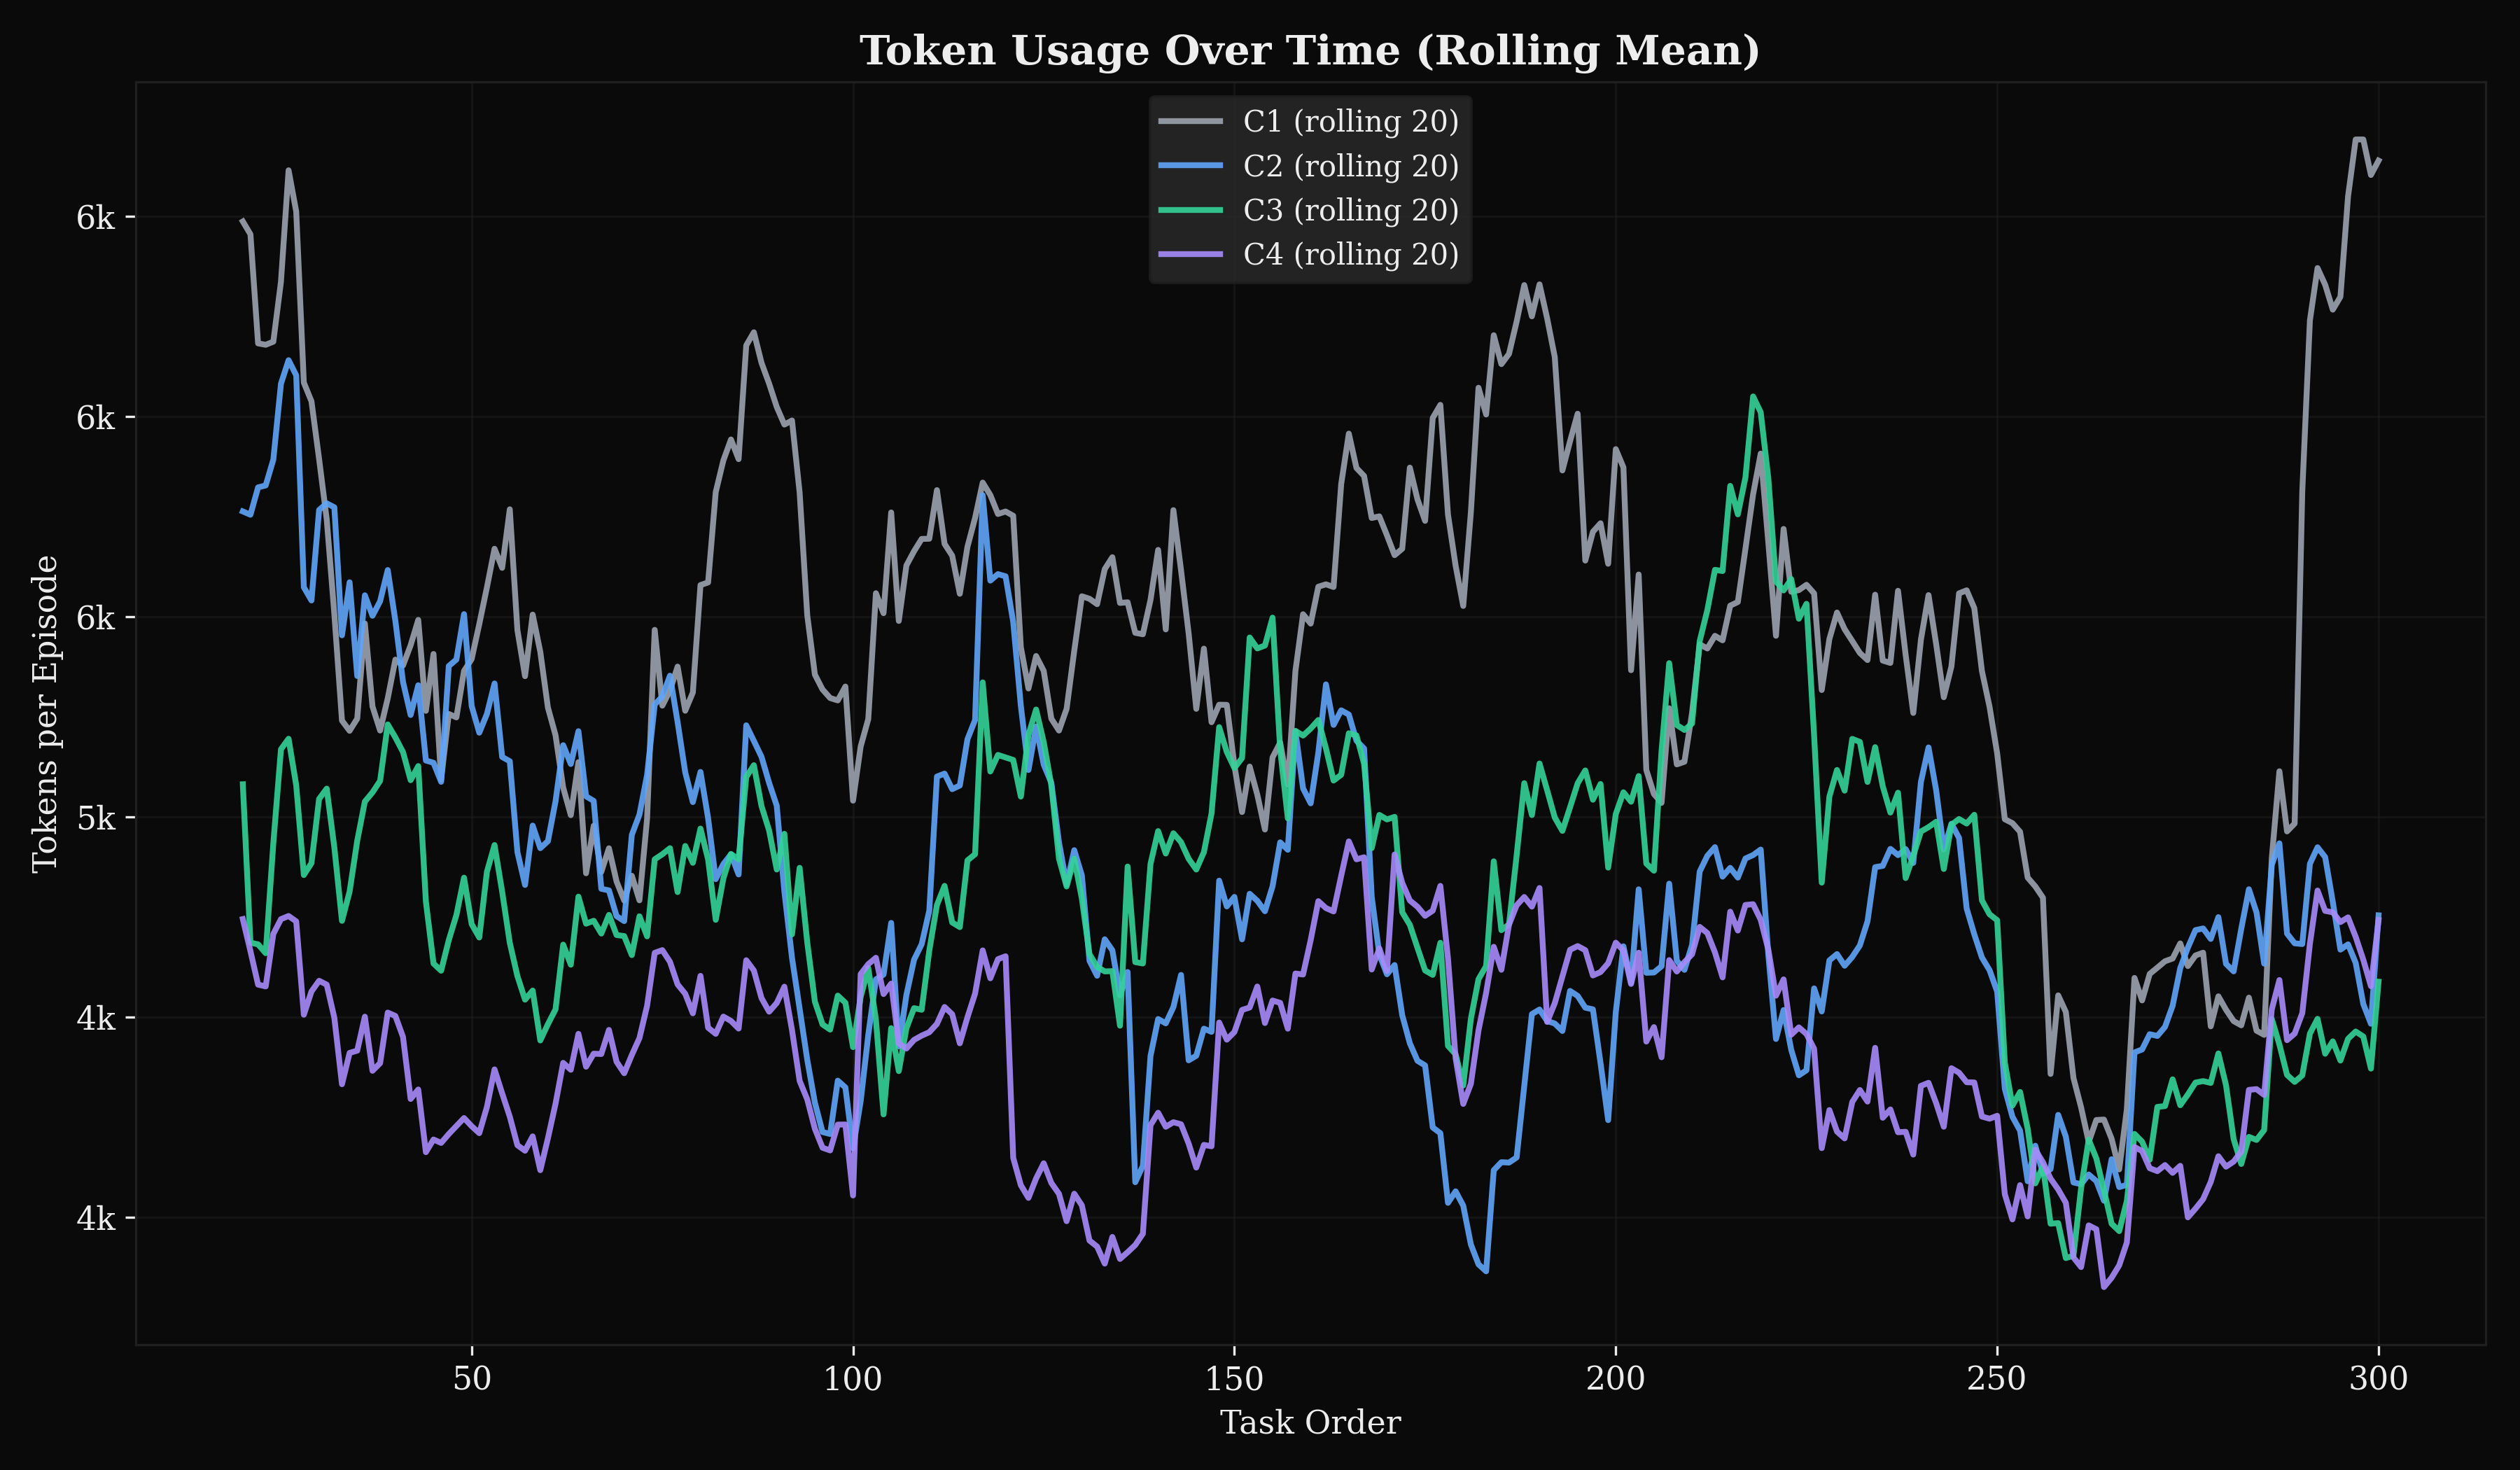
\includegraphics[width=\columnwidth]{../results/figures/figA2_token_trend.png}
\caption{Token consumption trend over episodes. No systematic drift is visible, confirming the absence of in-context learning effects or reward hacking.}
\label{fig:token_trend}
\end{figure}

\begin{figure}[t]
\centering
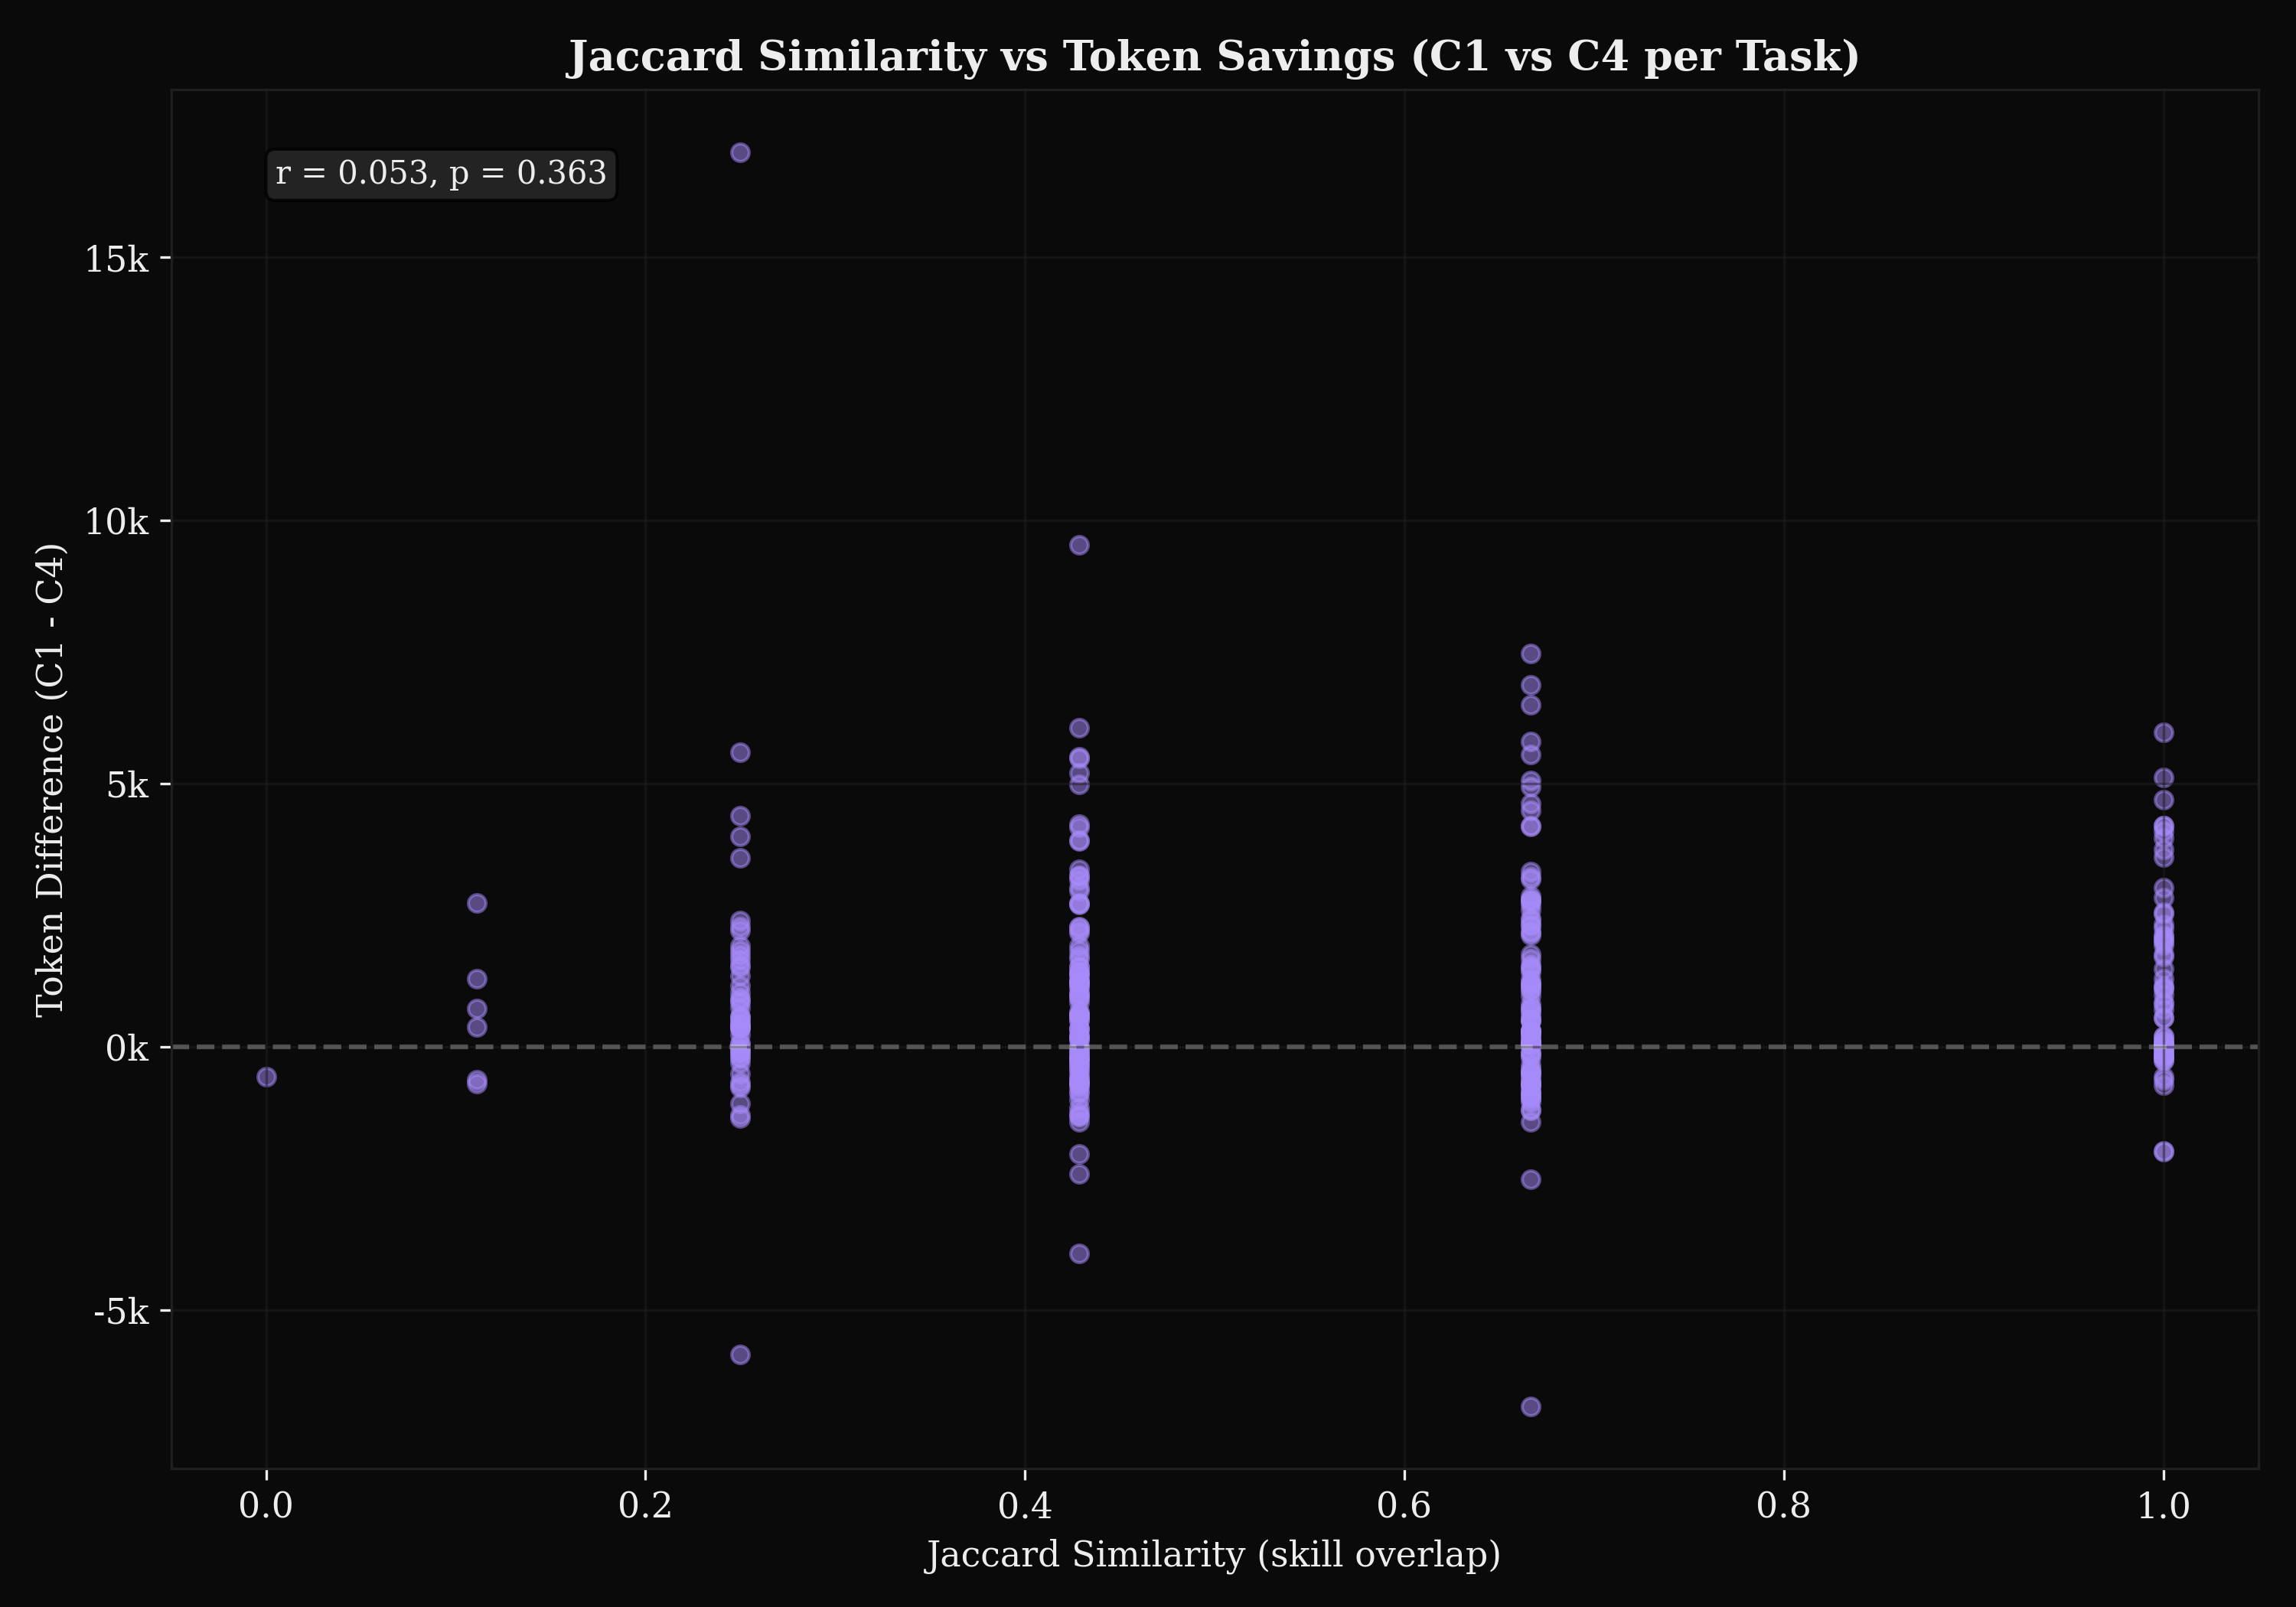
\includegraphics[width=\columnwidth]{../results/figures/figA4_jaccard_vs_tokens.png}
\caption{Relationship between Jaccard overlap and token consumption. Higher overlap (more similar retrievals) does not correlate with higher tokens, confirming that retrieval content is not the driver of token variation.}
\label{fig:jaccard_vs_tokens}
\end{figure}

\begin{figure}[t]
\centering
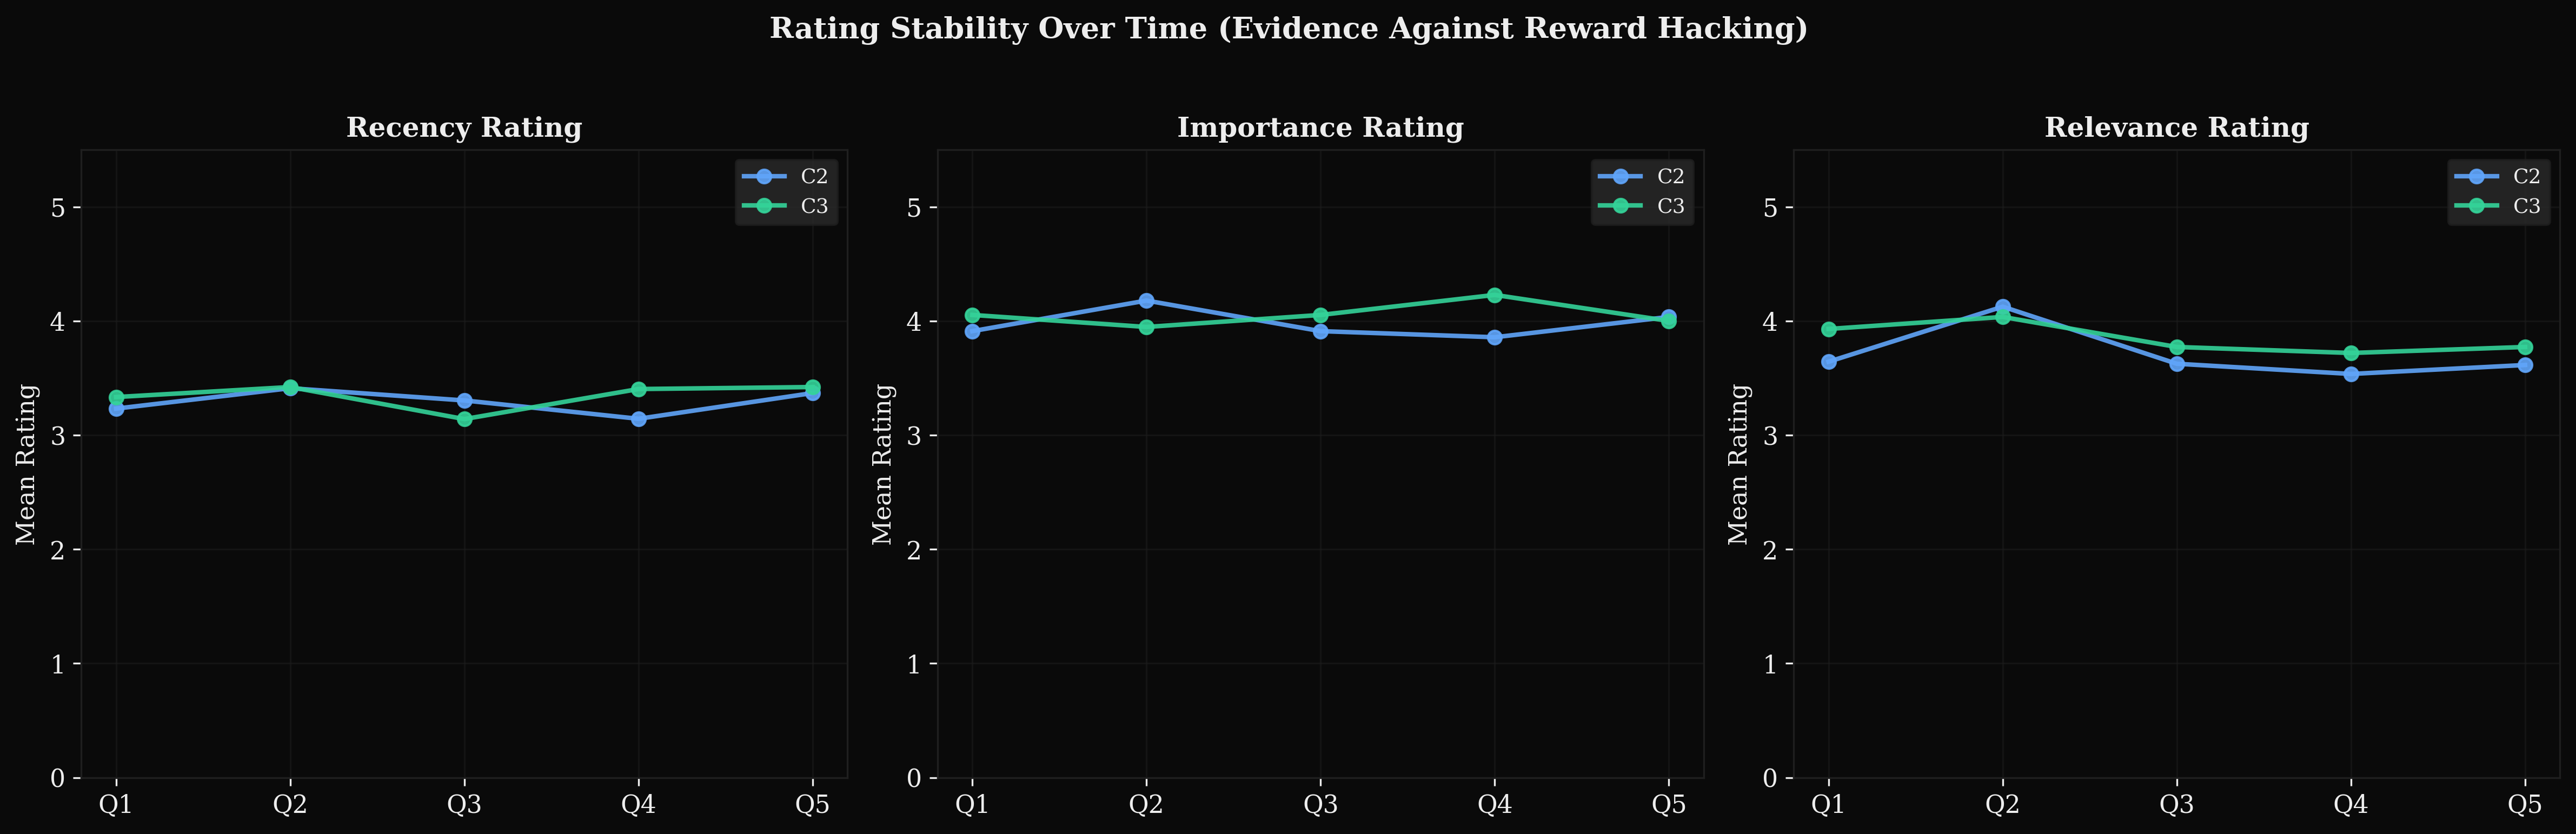
\includegraphics[width=\columnwidth]{../results/figures/figA6_rating_stability.png}
\caption{Dimension rating distributions across quartiles (first 25\%, last 25\% of episodes). Distributions are statistically indistinguishable ($p > 0.3$, KS test), confirming the absence of reward drift or in-context reward hacking.}
\label{fig:rating_stability}
\end{figure}



\end{document}
